\documentclass[a4paper,12pt]{article} % добавить leqno в [] для нумерации слева
\usepackage[a4paper,top=1.3cm,bottom=2cm,left=1.5cm,right=1.5cm,marginparwidth=0.75cm]{geometry}
%%% Работа с русским языком
\usepackage{cmap}					% поиск в PDF
\usepackage[warn]{mathtext} 		% русские буквы в фомулах
\usepackage[T2A]{fontenc}			% кодировка
\usepackage[utf8]{inputenc}			% кодировка исходного текста
\usepackage[english,russian]{babel}	% локализация и переносы
\usepackage{physics}
\usepackage{multirow}
\usepackage{longtable}

%%% Нормальное размещение таблиц (писать [H] в окружении таблицы)
\usepackage{float}
\restylefloat{table}



\usepackage{graphicx}

\usepackage{wrapfig}
\usepackage{tabularx}

\usepackage{hyperref}
\usepackage[rgb]{xcolor}
\hypersetup{
	colorlinks=true,urlcolor=blue
}

\usepackage{pgfplots}
\pgfplotsset{compat=1.9}

%%% Дополнительная работа с математикой
\usepackage{amsmath,amsfonts,amssymb,amsthm,mathtools} % AMS
\usepackage{icomma} % "Умная" запятая: $0,2$ --- число, $0, 2$ --- перечисление

%% Номера формул
\mathtoolsset{showonlyrefs=true} % Показывать номера только у тех формул, на которые есть \eqref{} в тексте.

%% Шрифты
\usepackage{euscript}	 % Шрифт Евклид
\usepackage{mathrsfs} % Красивый матшрифт

%% Свои команды
\DeclareMathOperator{\sgn}{\mathop{sgn}}

%% Перенос знаков в формулах (по Львовскому)
\newcommand*{\hm}[1]{#1\nobreak\discretionary{}
	{\hbox{$\mathsurround=0pt #1$}}{}}

\date{\today}

\usepackage{gensymb}

\usepackage{titlesec}
\titleformat{\section}{\filcenter\normalfont\Large\bfseries}{}{5pt}{}


\setlength{\topmargin}{-1in}
\setlength{\textheight}{9.5in}
\setlength{\oddsidemargin}{-0.7in}
\setlength{\evensidemargin}{-0.7in}
\setlength{\textwidth}{7.5in}
\setlength{\parindent}{2ex}
\setlength{\parskip}{1ex}

\newcommand{\HRule}{\rule{\linewidth}{0.5mm}}

\usepackage{fancyhdr}
\pagestyle{fancy} %% отвечает за колонтитулы
\fancyhead{}

\renewcommand{\numberline}[1]{}

\addtocontents{toc}{\unexpanded{\unexpanded{{%
  \itshape\footnotesize
	\HRule \\
  \par\bigskip
}}}}


\begin{document}


\begin{titlepage}
	\begin{center}
		{\large МОСКОВСКИЙ ФИЗИКО-ТЕХНИЧЕСКИЙ ИНСТИТУТ (НАЦИОНАЛЬНЫЙ ИССЛЕДОВАТЕЛЬСКИЙ УНИВЕРСИТЕТ)}
	\end{center}
	\begin{center}
		{\large Физтех-школа прикладной математики и информатики}
	\end{center}
	
	
	\vspace{6.5cm}
	{\huge
		\begin{center}
			{\bf Заметки к лекциям по многомерному анализу интегралам и рядам.}\\
			
		\end{center}
	}
	\vspace{7cm}
	\begin{flushright}
		{\LARGE Лектор:\\ Гусев Н. А. \\
			\vspace{0.2cm}

			}
	\end{flushright}
	\vspace{8cm}
\end{titlepage}



\tableofcontents
\newpage


\newpage
\begin{LARGE}
  \begin{center}
    \section{МА-28. Евклидова топология в $\mathbb{R}^{d}$ }
  \end{center}
\end{LARGE}
\HRule \\

\textbf{Окрестности точек и сходимость последовательностей}\\
Напомним, что $\varepsilon$-окрестностью точки $x=(x(1), x(2), \ldots, x(d)) \in \mathbb{R}^{d}$ называется множество

$$
U_{\varepsilon}(x):=\left\{y \in \mathbb{R}^{d}:|y-x|<\varepsilon\right\}
$$

где

$$
|y-x|=\sqrt{\sum_{k=1}^{d}|y(k)-x(k)|^{2}}
$$

В случае $d=1$ имеем $U_{\varepsilon}(x)=(x-\varepsilon, x+\varepsilon)$, а при $d>1$ множество $U_{\varepsilon}(x)$ представляет собой шар радиуса $\varepsilon$ с центром в точке $x$ (при этом сфера радиуса $\varepsilon$ с центром в $x$ в этот шар не включается).

Проколотой окрестностью точки $x \in \mathbb{R}^{d}$ называется множество $\stackrel{\circ}{U}_{\varepsilon}(x):=U_{\varepsilon}(x) \backslash$ $\{x\}$

Дополнением множества $E \subset \mathbb{R}^{d}$ называется множество $E^{c}:=\mathbb{R}^{d} \backslash E$.

Сходимость последовательностей точек в $\mathbb{R}^{d}$ определяется так же, как в одномерном случае. А именно, последовательность $\left\{x_{n}\right\} \subset \mathbb{R}^{d}$ сходится к $x \in \mathbb{R}^{d}$ при $n \rightarrow \infty$, если для любого $\varepsilon>0$ существует $N \in \mathbb{N}$ такое, что для всех $n>N$ выполнено $x_{n} \in$ $U_{\varepsilon}(x)$

\textbf{Утверждение 1:} Последовательность $\left\{x_{n}\right\} \subset \mathbb{R}^{d}$ сходится к $x \in \mathbb{R}^{d}$ при $n \rightarrow \infty$ тогда и только тогда, когда

$$
\left|x-x_{n}\right| \rightarrow 0
$$

$n p u n \rightarrow \infty$

\textbf{Доказательство:}\\
Утверждение очевидно, так как по определению условие $x_{n} \in U_{\varepsilon}(x)$ равносильно тому, что $\left|x-x_{n}\right|<\varepsilon$
покомпонентной сходимости (сходимости координат):

\textbf{Утверждение 2:} Последовательность $\left\{x_{n}\right\} \subset \mathbb{R}^{d}$ сходится к $x \in \mathbb{R}^{d}$ при $n \rightarrow \infty$ тогда и только тогда, когда для каждого $k \in \overline{1, d}$ выполнено

$$
x_{n}(k) \rightarrow x(k)
$$

$n p u n \rightarrow \infty$

\textbf{Доказательство:}\\
Необходимость вытекает из того, что для каждого $k \in \overline{1, d}$ выполнено

$$
\left|x_{n}(k)-x(k)\right| \leq\left|x_{n}-x\right|
$$

Достаточность следует из того, что

$$
\left|x_{n}-x\right| \leq \sqrt{d} \max _{1 \leq k \leq d}\left|x_{n}(k)-x(k)\right|
$$

\textbf{Внутренность и замыкание множества}\\
\textbf{Определение 3:} Пусть $E \subset \mathbb{R}^{d}$ и $x \in \mathbb{R}^{d}$.

\begin{enumerate}
  \item Если существует $\varepsilon>0$ такое, что $U_{\varepsilon}(x) \subset E$, то $x$ называется внутренней точкой множества $E$.
\end{enumerate}

\begin{itemize}
  \item Множество всех внутренних точек множества $E$ называется внутренностью Eи обозначается int $E$.
\end{itemize}

\begin{enumerate}
  \setcounter{enumi}{1}
  \item Если для любого $\varepsilon>0$ выполнено $U_{\varepsilon}(x) \cap E \neq \emptyset$, то $x$ называется точкой прикосновения множества $E$.
\end{enumerate}

\begin{itemize}
  \item Множество всех точек прикосновения множества E называется замыканием множества $E$ и обозначается $\bar{E}$.
\end{itemize}

По определению для любого множества $E$ выполнено

$$
\operatorname{int} E \subset E \subset \bar{E}
$$

Например, для множества $E=[0,1) \cup\{2\}$ выполнено:

$$
\operatorname{int} E=(0,1), \quad \bar{E}=[0,1] \cup\{2\}
$$

\textbf{Утверждение 4:} Пусть $E \subset \mathbb{R}^{d} u x \in \mathbb{R}^{d}$.

\begin{enumerate}
  \item Точка $x$ является внутренней точкой множества $E$ тогда и только тогда, когда для любой последовательности $\left\{x_{n}\right\}$ точек из $\mathbb{R}^{d}$, сходящейся к $x$, существует $N \in \mathbb{N}$ такое, что для всех $n>N$ выполнено $x_{n} \in E$.

  \item Точка $x$ является точкой прикосновения множества $E$ тогда и только тогда, когда существует последовательность $\left\{x_{n}\right\}$ точек из $E$, сходящаяся к $x$ при $n \rightarrow \infty$

\end{enumerate}

\textbf{Доказательство:}\\
\begin{enumerate}
  \item Необходимость следует из определения внутренней точки. Обратно, если точка $x$ не является внутренней, то для каждого $n \in \mathbb{N}$ в $1 / n$-окрестности $x$ найдётся точка $x_{n}$, не принадлежащая $E$. Тогда мы получаем последовательность точек из дополнения $E$, сходящуюся к $x$, что противоречит предположенному свойству.

  \item Достаточность следует из определения точки прикосновения. Обратно, если точка $x$ является точкой прикосновения множества $E$, то для каждого $n \in \mathbb{N}$ существует точка $x_{n} \in E$, принадлежащая $1 / n$-окрестности точки $x$. По построению $x_{n} \rightarrow x$ при $n \rightarrow \infty$.

\end{enumerate}

\textbf{Открытые и замкнутые множества}\\
\textbf{Определение 5:} Множество $E \subset \mathbb{R}^{d}$ называется

\begin{itemize}
  \item открытым, если $E=\operatorname{int} E$

  \item замкнутым, если $E=\bar{E}$.

\end{itemize}

Например, для любых $x \in \mathbb{R}^{d}$ и $\varepsilon>0$ множество $U_{\varepsilon}(x)$ открыто. Действительно, для любой точки $y \in U_{\varepsilon}(x)$ существует $\delta:=\varepsilon-|x-y|$ такое, что $U_{\delta}(y) \subset U_{\varepsilon}(x)$. Аналогично, множество $P_{\varepsilon}(x):=\left\{y \in \mathbb{R}^{d}:|y-x| \leq \varepsilon\right\}$ замкнуто.

В силу (1) можно сказать, что множество открыто тогда и только тогда, когда все его точки - внутренние. Аналогично, множество замкнуто тогда и только тогда, когда содержит все свои точки прикосновения. Сразу из определения следует, что внутренность любого множества представляет собой открытое множество, а замыкание любого множества представляет собой замкнутое множество.

$$
\bar{E}=\left(\operatorname{int} E^{c}\right)^{c}
$$

\textbf{Доказательство:}\\
Точка $x \in \mathbb{R}^{d}$ не является точкой прикосновения множества $E$ тогда и только тогда, когда существует $\varepsilon>0$ такое, что $U_{\varepsilon}(x) \cap E=\emptyset$. Последнее равносильно тому, что $U_{\varepsilon}(x) \subset E^{c}$, то есть $x \in \operatorname{int} E^{c}$. Значит $(\bar{E})^{c}=\operatorname{int} E^{c}$. Взяв дополнение, получим (2).

\textbf{Граница множества. Предельные и изолированные точки}\\
\textbf{Определение 7:} Пусть $E \subset \mathbb{R}^{d} u x \in \mathbb{R}^{d}$.

\begin{enumerate}
  \item Если для любого $\varepsilon>0$ выполнено $U_{\varepsilon}(x) \cap E \neq \emptyset$ и $U_{\varepsilon}(x) \cap E^{c} \neq \emptyset$, mо $x$ называется граничной точкой множества $E$.
  \item Множество всех граничных точек множества $E$ называется границей $E$ и обозначается $\partial E$.


  \item Если для любого $\varepsilon>0$ выполнено $\stackrel{\circ}{U}_{\varepsilon}(x) \cap E \neq \emptyset$, то $x$ называется предельной точкой множества $E$.

  \item Если $x \in E$ и существует $\varepsilon>0$ такое, что $\stackrel{O}{U}_{\varepsilon}(x) \cap E=\emptyset$, то $x$ называется изолированной точкой множества $E$.

\end{enumerate}

Например, если $d=1$ и $E=[0,1) \cup\{2\}$, то $[0,1]$ является множеством всех предельных точек множества $E$, а точка 2 является единственной изолированной точкой множества $E$.

\textbf{Теорема 8:} Для любого $E \subset \mathbb{R}^{d}$ выполнено

$$
\partial E=\left(\operatorname{int} E \sqcup \operatorname{int} E^{c}\right)^{c}
$$

Kpome того,

$$
\bar{E}=\operatorname{int} E \sqcup \partial E=E \cup \partial E
$$

\textbf{Доказательство:}\\
В силу (1) имеем $\operatorname{int} E \subset E$ и int $E^{c} \subset E^{c}$, поэтому множества int $E$ и int $E^{c}$ не пересекаются. Точка $x \in \mathbb{R}^{d}$ не принадлежит int $E \sqcup \operatorname{int} E^{c}$ тогда и только тогда, когда в любой её $\varepsilon$-окрестности найдётся хотя бы одна точка из $E$ и хотя бы одна точка из $E^{c}$. Это по определению границы и означает, что $x \in \partial E$. Заметим, что $\partial E \subset \bar{E}$, так как по определению в любой $\varepsilon$-окрестности точки границы $E$ содержится хотя бы одна точка множества $E$. При этом точка $x$ принадлежит $\bar{E} \backslash \partial E$ тогда и только тогда, когда некоторая её окрестность лежит во множестве $E$. Значит $\bar{E} \backslash \partial E=\operatorname{int} E$

Наконец, $E \subset \bar{E}$ и $\partial E \subset \bar{E}$, поэтому

$$
\bar{E}=\operatorname{int} E \sqcup \partial E \subset E \cup \partial E \subset \bar{E}
$$

Отсюда видно, что $\bar{E}=E \cup \partial E$.

Таким образом, для любого множества $E \subset \mathbb{R}^{d}$ множество $\mathbb{R}^{d}$ разбивается на 3 попарно непересекающихся подмножества: $\operatorname{int} E, \partial E$ и int $E^{c}$. Например, если $d=1$ и $E=(-\infty, 0) \cup(\mathbb{Q} \cap[0,1])$, то это разбиение имеет вид

\begin{figure}[H]
  \begin{center}
      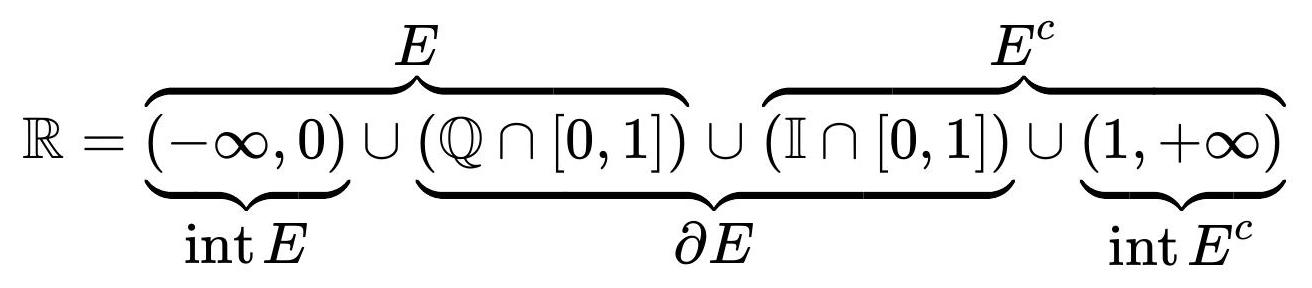
\includegraphics[width=11cm]{2023_05_20_70c2606c431f82d3de98g-05.jpg}
  \end{center}
\end{figure}

\textbf{Теоретико-множественные свойства открытых и замкнутых множеств}\\
Обсудим свойства открытых и замкнутых множеств, связанные с операциями объединения, пересечения и взятия дополнения. Прежде всего отметим, что понятие замкнутости множества можно было бы эквивалентно определить иначе:

\textbf{Теорема 9:} Множество $E$ замкнуто тогда и только тогда, когда его дополнение открыто.

\textbf{Доказательство:}\\
В силу (2) равенство $E=\bar{E}$ равносильно тому, что $E=\left(\operatorname{int} E^{c}\right)^{c}$, то есть $E^{c}=\operatorname{int} E^{c}$. Последнее равносильно открытости $E^{c}$.

\textbf{Теорема 10:} Объединение любого семейства $\mathscr{G}$ открытых множеств открыто. Если, кроме того, семейство $\mathscr{G}$ конечно, то и пересечение $\mathscr{G}$ открыто.

\textbf{Доказательство:}\\
Пусть $E:=\bigcup \mathscr{G}$. Напомним, по определению объединения семейства множеств точка $x$ принадлежит множеству $E$ тогда и только тогда, когда она принадлежит некоторому элементу $G$ семейства $\mathscr{G}$. Так как множество $G$ открыто, то существует $\varepsilon>0$ такое, что $U_{\varepsilon}(x) \subset G$. Но $G \subset E$, а значит $x \in \operatorname{int} E$. Следовательно, $E$ открыто.

Теперь предположем, что $\mathscr{G}=\left\{G_{1}, \ldots, G_{n}\right\}$ (для некоторого $n \in \mathbb{N}$ ). Пусть $P=$ $\bigcap G=G_{1} \cap \ldots \cap G_{n}$ и $x \in P$. Тогда для каждого $k \in \overline{1, n}$ точка $x$ принадлежит открытому множеству $G_{k}$. Значит найдётся $\varepsilon_{k}>0$ такое, что $U_{\varepsilon_{k}}(x) \subset G_{k}$. Взяв $\varepsilon:=$ $\min \left(\varepsilon_{1}, \ldots, \varepsilon_{n}\right)$ получим $U_{\varepsilon}(x) \subset G_{k}$ для каждого $k \in \overline{1, n}$. Значит $U_{\varepsilon}(x) \subset P$. Следовательно $P$ открыто.

Иначе говоря, если для каждого элемента $a$ некоторого множества $A$ дано открытое множество $G_{a}$, то множество $\bigcup_{a \in A} G_{a}$ открыто. Даже если множество индексов $A$ несчётно. Например, если $A=[0,1]$ и $G_{a}=(a, a+1)$ для всех $a \in A$, то $\bigcup_{a \in A} G_{a}=$ $(0,2)$ действительно открыто.

Если множество индексов $A$ конечно, то и множество $\bigcap_{a \in A} G_{a}$ открыто. Но если $A$ бесконечно, то множество $\bigcap_{a \in A} G_{a}$ не обязано быть открытым. Например, если $A=\mathbb{N}$ и $G_{a}=(-1 / a, 1 / a)$ для любого $a \in A$, то $\bigcap_{a \in A} G_{a}=\{0\}$ не является открытым.

\textbf{Утверждение 11:} Для любого множества $E$ его внутренность является наибольшим по вложению открытым подмножеством множества E. Кроме того, int $E$ совпадает с объединением всех открытых подмножеств множества $E$.

\textbf{Доказательство:}\\
Пусть $M$ - объединение семейства

$$
\mathscr{G}:=\left\{G \subset \mathbb{R}^{d}: G \text { открыто, } G \subset E\right\}
$$

Данное семейство состоит из открытых множеств, значит по теореме 10 множество $M$ открыто. Кроме того, для любого $G \in \mathscr{G}$ выполнено $G \subset E$, поэтому $M \subset E$. Таким образом, множество $M$ принадлежит семейству $\mathscr{G}$.

По определению объединения для любого $G \in \mathscr{G}$ выполнено $G \subset M$. Значит $M$ является наибольшим по вложению открытым подмножеством множества $E$. (Отметим, что другого такого открытого множества $M^{\prime}$ не существует, поскольку в силу минимальности по вложению мы имели бы $M \subset M^{\prime}$ и $M^{\prime} \subset M$, откуда $M=M^{\prime}$.)

Все точки каждого $G \in \mathscr{G}$ являются внутренними точками $E$ (так как $G$ открыто и $G \subset$ $E)$, а значит $G \subset \operatorname{int} E$. Тогда по определению объединения $M \subset \operatorname{int} E$. С другой стороны, ясно что int $E$ является одним из элементов семейства $\mathscr{G}$. Тогда по определению объединения int $E \subset M$. Из полученных вложений заключаем, что $M=\operatorname{int} E$ Следствие 12. Для любого множества $E$ его замыкание является наименьшим по вложению замкнутым множеством, подмножеством которого является Е. Кроме того, $\bar{E}$ совпадает с пересечением всех замкнутых множеств, включающих в себя $E$.

\textbf{Доказательство:}\\
В силу теоремы 9 замкнутое множество $F$ содержит $E$ тогда и только тогда, когда открытое множество $F^{c}$ лежит в $E^{c}$. Иначе говоря, множество $F$ принадлежит семейству

$$
\mathscr{F}:=\left\{F \subset \mathbb{R}^{d}: F \text { замкнуто, } E \subset F\right\}
$$

тогда и только тогда, когда его дополнение принадлежит семейству

$$
\mathscr{G}:=\left\{G \subset \mathbb{R}^{d}: G \text { открыто, } G \subset E^{c}\right\}
$$

Тогда

$$
\bigcap_{F \in \mathscr{F}} F=\bigcap_{F^{c} \in \mathscr{G}}\left(F^{c}\right)^{c}=\bigcap_{G \in \mathscr{G}} G^{c}=\left(\bigcup_{G \in \mathscr{G}} G\right)^{c}=\left(\operatorname{int} E^{c}\right)^{c}=\bar{E} .
$$

Отсюда по определению пересечения имеем $\bar{E} \subset F$ для любого $F \in \mathscr{F}$. С другой стороны, $\bar{E}$ замкнуто и $E \subset \bar{E}$, значит $\bar{E} \in \mathscr{F}$. Таким образом, $\bar{E}$ является наименьшим по вложению элементом семейства $\mathscr{F}$.

\textbf{Отделимось замкнутых множеств}\\
Открытое множество $G \subset \mathbb{R}^{d}$ называется (открытой) окрестностью точки $x \in \mathbb{R}^{d}$, если $x \in G$. Аналогично, открытое множество $G \subset \mathbb{R}^{d}$ называется (открытой) окрестностью множества $E \subset \mathbb{R}^{d}$, если $E \subset G$.

Легко видеть, что у любых двух различных точек $x, y \in \mathbb{R}^{d}$ имеются непересекающиеся окрестности. Действительно, если $|x-y|=\varepsilon>0$, то $G_{1}=U_{\varepsilon / 2}(x)$ и $G_{2}=U_{\varepsilon / 2}(x)$ открыты и не пересекаются, и при этом $x \in G_{1}$ и $y \in G_{2}$.

Расстоянием от точки $x$ до непустого множества $E \subset \mathbb{R}^{d}$ называется число

$$
\rho(x, E):=\inf _{y \in E}|x-y|
$$

Аналогично, расстоянием между множествами $E, F \subset \mathbb{R}^{d}$ называется число

$$
\rho(E, F):=\inf _{x \in E, y \in F}|x-y| .
$$

Если $\rho(E, F)>0$, то непересекающиеся окрестности множеств $E$ и $F$ можно построить аналогично тому, как это делалось для двух точек. Оказывается, что непересекающиеся окрестности можно построить для любых двух непересекающихся замкнутых множеств (даже если расстояние между ними равно нулю):

\textbf{Утверждение 13:} Если замкнутые множества $F_{1}$ и $F_{2}$ не пересекаются, то существуют непересекающиеся открытые множества $G_{1}$ и $G_{2}$ такие, что $F_{1} \subset G_{1}$ и $F_{2} \subset G_{2}$.

\textbf{Доказательство:}\\
Действительно, так как $F_{1} \subset F_{2}^{c}$, то для каждого $x \in F_{1}$ существует $\varepsilon=\varepsilon(x)>0$ такое, что $U_{\varepsilon(x)}(x) \subset F_{2}^{c}$. Аналогично, для каждого $y \in F_{2}$ существует $\delta=\delta(y)>0$ такое, что $U_{\delta(y)}(y) \subset F_{1}^{c}$. Возьмём $G_{1}:=\bigcup_{x \in F_{1}} U_{\varepsilon(x) / 2}(x)$ и $G_{2}:=\bigcap_{x \in F_{2}} U_{\delta(y) / 2}(y)$. Ясно, что $G_{1}$ и $G_{2}$ открыты. Если существует $z \in G_{1} \cap G_{2}$, то существуют $x \in F_{1}$ и $y \in F_{2}$ такие, что $z \in U_{\varepsilon(x) / 2}(x) \cap U_{\delta(y) / 2}(y)$. Тогда

$$
|x-y| \leq|x-z|+|z-y|<(\varepsilon(x)+\delta(y)) / 2<\max (\varepsilon(x), \delta(y)) .
$$

Значит либо $x \in U_{\delta(y)}(y)$, либо $y \in U_{\varepsilon(x)}(x)$, что противоречит определению $\varepsilon$ и $\delta$.

\textbf{Структура открытых подмножеств вещественной прямой}\\
Ясно, что любое объединение интервалов представляет собой открытое множество. Верно и обратное: любое открытое множество $E \subset \mathbb{R}$ можно представить в виде объединения интервалов. Действительно, по определению открытого множества для любого $x \in E$ существует $\varepsilon=\varepsilon(x)>0$ такое, что $U_{\varepsilon(x)}(x) \subset E$. Тогда

$$
E=\bigcup_{x \in E}\{x\} \subset \bigcup_{x \in E} U_{\varepsilon(x)}(x) \subset E
$$

значит $E=\bigcup_{x \in E} U_{\varepsilon(x)}(x)$. Таким образом, $E$ представлено в виде объединения некоторого семейства открытых интервалов, в общем случае несчётного. Оказывается, что всегда можно ограничиться счётным семейством, а сами интервалы выбирать попарно непересекающимися:

\textbf{Теорема 14:} Любое открытое множество $E \subset \mathbb{R}$ можно представить в виде объединения не более чем счётного семейства попарно непересекающихся интервалов.

\textbf{Доказательство:}\\
Для каждой точки $x \in E$ выберем максимальный по вложению интервал $I_{x}$ такой, что $x \in I_{x} \subset E$. Для этого рассмотрим семейство $\mathcal{F}_{x}:=\{(a, b): a, b \in \overline{\mathbb{R}}, x \in(a, b) \subset$ $E\}$ и возьмём $I_{x}:=\bigcup \mathcal{F}_{x}$. Множество $I_{x}$ открыто (как объединение открытых множеств). Кроме того, $I_{x}$ является непустым промежутком, так как для любого $\xi \in I_{x}$ отрезок $[x, \xi]$ (или $[\xi, x]$ если $\xi<x$ ) лежит в некотором интервале из $\mathcal{F}_{x}$ и, следовательно, лежит в $I_{x}$. Тогда $I_{x} \in \mathcal{F}_{x}$. Так как для любого $J \in \mathcal{F}_{x}$ выполнено $J \subset$ $I_{x}$, то $I_{x}$ является наибольшим по вложению элементом $\mathcal{F}_{x}$.

Заметим, что если $x, y \in E$, то либо $I_{x} \cap I_{y}=\emptyset$, либо $I_{x}=I_{y}$. Действительно, если $I_{x} \cap I_{y} \neq \emptyset$, то $I:=I_{x} \cup I_{y}$ является интервалом, лежит в $E$ и содержит точки $x$ и $y$. Последнее возможно лишь в случае, когда $I_{x}=I_{x} \cup I_{y}=I_{y}$ (иначе получаем противоречие максимальности интервалов $I_{x}$ и $\left.I_{y}\right)$.

Рассмотрим семейство $\mathcal{G}:=\left\{I_{x}: x \in E\right\}$. Так как $\mathcal{G}$ является дизъюнктным семейством непустых интервалов, то $\mathcal{G}$ не более чем счётно.

Наконец, для любого $x \in E$ выполнено $I_{x} \subset E$, поэтому $\bigcup \mathcal{G} \subset E$. С другой стороны, $E=\bigcup_{x \in E}\{x\} \subset \bigcup_{x \in E} I_{x}=\bigcup \mathcal{G}$. Значит $E=\bigcup \mathcal{G}$, что и требовалось доказать.

Следствие 15. Множества $\emptyset$ и $\mathbb{R}$ являются единственными множествами, которые открыты и замкнуты одновременно.

\textbf{Доказательство:}\\
Предположим, что $E \subset \mathbb{R}$ непусто, открыто и замкнуто одновременно. Тогда $E^{c}$ открыто. Возьмём точку $x \in E$ и выберем для неё максимальный по вложению интервал $I_{x}$ такой, что $x \subset I_{x} \subset E$. Обозначим $\alpha:=\inf I_{x}, \beta:=\sup I_{x}$. Если $\beta \in \mathbb{R}$, то $\beta \in E^{c}$. Но тогда существует $\delta>0$ такое, что $(\beta-\delta, \beta+\delta) \subset E^{c}$. Это противоречит тому, что $(\alpha, \beta) \subset E$. Таким образом, $\beta=+\infty$ и из аналогичных соображений $\alpha=-\infty$




\newpage
\begin{LARGE}
  \begin{center}
    \section{МА-30. Компакты в $\mathbb{R}^{d}$ }
  \end{center}
\end{LARGE}
\HRule \\

Множество $E \subset \mathbb{R}^{d}$ называется ограниченным, если оно лежит в некотором шаре. Это эквивалентно существованию константы $C>0$ такой, что $|x| \leq C$ для всех $x \in E$.

\textbf{Определение 1:} Множество $K \subset \mathbb{R}^{d}$ называется компактом, если оно ограничено и замкнуто.

\textbf{Теорема 2:} (свойство Больцано-Вейерштрасса). Множество $K \subset \mathbb{R}^{d}$ является компактом тогда и только тогда, когда из любой последовательности точек $x_{n}$ множества $K$ можно выделить подпоследовательность, сходящуюся к некоторой точке множества $K$.

\textbf{Доказательство:}\\
Необходимость. Пусть $x_{n} \in K$ для всех $n \in \mathbb{N}$. Так как $K$ ограничено, то числовая последовательность $\left\{x_{n}(1)\right\}_{n \in \mathbb{N}}$ также ограничена. По теореме Больцано-Вейерштрасса из неё можно выделить сходящуюся подпоследовательность $x_{n_{k}}(1)$. Аналогично, из ограниченной числовой последовательности $x_{n_{k}}(2)$ можно выделить сходящуюся подпоследовательность $x_{n_{k_{\ell}}}(2)$. Переходя к следующим компонентам и выбирая сходящуюся подпоследовательность получим строго возрастающую последовательность индексов $\left\{m_{k}\right\}_{k} \subset \mathbb{N}$ такую, что для каждого $j \in \overline{1, d}$ последовательность $\left\{x_{m_{k}}(j)\right\}$ сходится при $k \rightarrow \infty$. Следовательно, последовательность $\left\{x_{m_{k}}\right\}$ сходится к некоторой точке $x \in \mathbb{R}^{d}$ при $k \rightarrow \infty$. Так как $K$ замкнуто, то $x \in K$.

Достаточность. Пусть $K$ - компакт. Если $K$ неограничено, то можно выбрать последовательность точек $x_{n} \in K$ так, что $\left|x_{n}\right| \rightarrow \infty$ при $n \rightarrow \infty$. Из такой последовательности, очевидно, нельзя выбрать подпоследовательность, сходящуюся к некоторой точке $x \in \mathbb{R}^{d}$. Противоречие. Значит $K$ ограничено.

Пусть последовательность точек $\left\{x_{n}\right\}_{n \in \mathbb{N}}$ лежит в $K$ и сходится к $x \in \mathbb{R}^{d}$ при $n \rightarrow \infty$. По определению компакта мы можем выделить подпоследовательность $\left\{x_{n_{k}}\right\}_{k \in \mathbb{N}}$, сходящуюся к некоторой точке множества $K$. Но $x_{n_{k}} \rightarrow x$ при $k \rightarrow \infty$. Поэтому $x \in$ $K$. Значит $K$ замкнуто.\\ \textbf{Определение 3:} Семейство $\mathscr{F}$ называется покрытием множества $E$, если для каждого $x \in E$ существует множество $A \in \mathscr{F}$ такое, что $x \in A$. Семейство $\mathscr{G} \subset \mathscr{F}$ называется подпокрытием множества $E$, если $\mathscr{G}$ также является покрытием множества $E$.

Покрытие $\mathscr{F}$ множества $E \subset \mathbb{R}^{d}$ называется открытым, если $\mathscr{F}$ состоит из открытых множеств.

Например, семейство $\mathscr{F}=\{(a-1, a+1): a \in \mathbb{I}\}$ является (несчётным) открытым покрытием отрезка $E=[-1,1]$. Семейство $\mathscr{G}=\left\{\left(-\frac{1}{\sqrt{2}}-1,-\frac{1}{\sqrt{2}}+1\right),\left(\frac{1}{\sqrt{2}}-\right.\right.$ $\left.\left.1, \frac{1}{\sqrt{2}}+1\right)\right\} \subset \mathscr{F}$ является (конечным) подпокрытием отрезка $E$.

\textbf{Теорема 4:} (лемма Гейне-Бореля). Множество $K \subset \mathbb{R}^{d}$ является компактом тогда и только тогда, когда из любого открытого покрытия множества $K$ можно выделить конечное подпокрытие.

\textbf{Доказательство:}\\
Достаточность. Рассмотрим открытое покрытие $\mathscr{F}=\left\{\left\{x \in \mathbb{R}^{d}:|x|<r\right\}: r>0\right\}$ множества $K$. Так как из $\mathscr{F}$ можно выделить конечное подпокрытие, то $K$ ограничено.

Пусть последовательность точек $\left\{x_{n}\right\}_{n \in \mathbb{N}} \subset K$ сходится к точке $x \in \mathbb{R}^{d}$. Если $x \notin K$, то семейство $\mathscr{F}=\left\{\left\{y \in \mathbb{R}^{d}:|x-y|>r\right\}: r>0\right\}$ покрывает $K$ и из него можно выделить конечное подпокрытие. Тогда для некоторого $r>0$ выполнено $K \subset\{y \in$ $\left.\mathbb{R}^{d}:|x-y|>r\right\}$. Значит для всех $n \in \mathbb{N}$ выполнено $\left|x-x_{n}\right|>r$, что противоречит сходимости $x_{n} \rightarrow x$ при $n \rightarrow \infty$.

Необходимость. Пусть $K$ - компакт и $\mathscr{F}=\left\{U_{a}\right\}_{a \in A}$ - его открытое покрытие, из которого нельзя выделить конечное подпокрытие. Так как $K$ ограничено, то оно лежит в некотором $d$-мерном параллелепипеде $P$.

Разделив каждую сторону $P$ пополам, получим $2^{d}$ параллелепипедов $P_{i}$. Если для каждого $i$ множество $K \cap P_{i}$ покрывается конечным набором элементов $\mathscr{F}$, то и всё множество $K$ можно покрыть конечным набором элементов $\mathscr{F}$, что противоречит сделанному предположению. Значит найдётся параллелепипед $Q_{1}$ такой, что $K \cap Q_{1}$ не покрывается никаким конечным набором элементов $\mathscr{F}$ (в частности, $K \cap Q_{1} \neq \emptyset$ ).

Теперь в качестве $P$ можно взять $Q_{1}$ и повторить сделанный шаг. Продолжая данный процесс, в итоге мы получим последовательность стягивающихся вложенных параллелепипедов $\left\{Q_{j}\right\}_{j \in \mathbb{N}}$ таких, что $K \cap Q_{j}$ не покрывается никаким конечным набором элементов $\mathscr{F}$. По теореме Кантора (строго говоря, её мы применяем к проекциям рассматриваемых параллелепипедов) существует единственная точка $x \in$ $\bigcap_{j=1}^{\infty} Q_{j}$. Так как $K \cap Q_{j} \neq \emptyset$, то $x \in \bar{K}$. В силу замкнутости $K$ заключаем, что $x \in$ $K$.

По определению покрытия существует $U \in \mathscr{F}$ такое, что $x \in U$. Но тогда при достаточно больших $j$ выполнено $Q_{j} \subset U$. (Действительно, так как $x \in U$, то существует $\varepsilon>0$ такое, что $U_{\varepsilon}(x) \subset U$. Тогда для того, чтобы $Q_{j} \subset U$ достаточно, чтобы каждая из сторон $Q_{j}$ была меньше $\varepsilon / \sqrt{d}$.)

В силу теорем 2 и 4 следующие 3 свойства множества $K \subset \mathbb{R}^{d}$ эквивалентны:

\begin{enumerate}
  \item $K$ ограничено и замкнуто.

  \item из любой последовательности элементов множества $K$ можно выделить подпоследовательность, сходящуюся к некоторому элементу множества $K$.

  \item из любого открытого покрытия множества $K$ можно выделить конечное подпокрытие.

\end{enumerate}

Забегая вперёд отметим, что эти три свойства эквивалентны только в случае евклидовой топологии. В общем случае за определение компактности берётся третье свойство, а второе свойство называется секвенциальной компактностью.

\textbf{Множество Кантора}\\
Простейшим примером компакта в $\mathbb{R}$ является отрезок $[0,1]$. Другой примера компакта - множество вида $\left\{\frac{1}{n}: n \in \mathbb{N}\right\} \cup\{0\}$. Может ли компакт быть несчётным и при этом не содержать ни одного отрезка положительной длины? Оказывается, что да. Для построения такого компакта $C$ начнём со множества $C_{0}:=[0,1]$. Исключив из $C_{0}$ интервал $\left(\frac{1}{3}, \frac{2}{3}\right)$ получим множество $C_{1}:=\left[0, \frac{1}{3}\right] \cup\left[\frac{2}{3}, 1\right]$. В каждом из двух отрезков, составляющих $C_{1}$, исключим интервал с центром в середине и длиной $1 / 9$. Продолжая по аналогии на $n$-ом шаге получим множество $C_{n}$, состоящее из $2^{n}$ попарно непересекающихся отрезков длины $3^{-n}$.

\textbf{Определение 5:} Множество $C:=\bigcap_{n=1}^{\infty} C_{n}$ называется (тонким) множеством Кантора.

\textbf{Утверждение 6:} Множество Кантора $C$ замкнуто, равномощно $\mathbb{R}$ и не включает в сем ни одного отрезка ненулевой длины.
ненулевой длины, следует из того, что в $C$ не входят числа вида $m / 2^{n}$, где $m, n \in \mathbb{N}$, а в любом отрезке ненулевой длины содержится хотя бы одно число такого вида.

	\newpage

	\begin{LARGE}
		\begin{center}
			\section{МА-31. Непрерывность функций. Связность и линейная связность}
		\end{center}
	\end{LARGE}
	\HRule \\


	\textbf{	Пределы по направлениям и по совокупности переменных.}\\
	Открытое множество $U \subset \mathbb{R}^{n}$ называется (открытой) окрестностью точки $x \in \mathbb{R}^{n}$, если $x \in U$.
	
	Рассмотрим отображение $f: \mathbb{R}^{n} \rightarrow \mathbb{R}^{m}$. По аналогии с одномерным случаем точка $y \in$ $\mathbb{R}^{m}$ называется пределом $f$ в точке $x \in \mathbb{R}^{n}$ (по совокупности переменных) если для любого $\varepsilon>0$ существует $\delta>0$ такое, что $f\left(\stackrel{\circ}{U}_{\delta}(x)\right) \subset U_{\varepsilon}(y)$. Обозначение: $y=\lim _{z \rightarrow x} f(z)$.
	
	Если отображение $f$ определено не на всём $\mathbb{R}^{n}$, а лишь на некотором подмножестве $E \subset$ $\mathbb{R}^{n}$, для которого $x$ является предельной точкой, то условие $f\left(\stackrel{\circ}{U}_{\delta}(x)\right) \subset U_{\varepsilon}(y)$ необходимо заменить на $f\left(E \cap \stackrel{\circ}{U}_{\delta}(x)\right) \subset U_{\varepsilon}(y)$; в этом случае говорят о пределе по множеству $E$. Чтобы это подчеркнуть, иногда используют обозначение $\lim _{E \ni z \rightarrow x} f(z)$.
	
	Если $a \in \mathbb{R}^{n}$ - ненулевой вектор, то предел $\lim _{t \rightarrow 0} f(x+a t)$, если он существует, называется пределом $f$ по направлению $a$. При $t \rightarrow \pm 0$ говорят об односторонних пределах по направлению.
	
	\textbf{Утверждение 1.} Если отображение $f$ имеет в точке $x \in \mathbb{R}^{n}$ предел $y \in \mathbb{R}^{m}$ (по совокупности переменных), то для любого ненулевого вектора $a \in \mathbb{R}^{n}$ отображение $f$ имеет предел по направлению $a$, равный $y$.
	
	\textbf{Доказательство:\\}
	По определению предела для любого $\varepsilon>0$ существует $\delta>0$ такое, что $f\left(\stackrel{\circ}{U}_{\delta}(x)\right) \subset$ $U_{\varepsilon}(y)$. Если $|t|<\delta /|a|$, то $x+a t \in U_{\delta}(x)$. Тогда $f(x+a t) \in U_{\varepsilon}(y)$.
	
	Обратное в общем случае не имеет места. Например, функция $f: \mathbb{R}^{2} \rightarrow \mathbb{R}$ вида
	
	$$
	f(x, y)= \begin{cases}1, & y=x^{2} \\ 0, & \text { иначе }\end{cases}
	$$
	
	не имеет предела в точке $0=(0,0)$, но для любого ненулевого вектора $a \in \mathbb{R}^{n}$ функция $f$ имеет предел по направлению $a$, равный нулю. Утверждение 2. Пусть отображение $f=f(x) \in \mathbb{R}^{m}$ определено в проколотой окрестности точки $x \in \mathbb{R}^{n}$. Пусть $y \in \mathbb{R}^{m}$. Для того, чтобы предел $f$ в точке $x$ (по совокупности переменных) был равен $y$ необходимо и достаточно, чтобы для любой дифференцируемой в нуле вектор-функции $g=g(t) \in \mathbb{R}^{n}$ такой, что $g(0)=x$ и $g^{\prime}(0) \neq$ 0, существовал $\lim _{t \rightarrow 0} f(g(t))=y$
	
	\textbf{Доказательство:\\}
	Не уменьшая общности пусть $x=0$ и $y=0$.
	
	\textit{Необходимость.}\\ Пусть $f(z) \rightarrow 0$ при $z \rightarrow 0$. Тогда для любого $\varepsilon>0$ существует $\delta>0$ такое, что при $0<|z|<\delta$ выполнено $|f(z)|<\varepsilon$. Для любой дифференцируемой в нуле (и, следовательно, непрерывной в нуле) вектор-функции $g=g(t) \in \mathbb{R}^{n}$ такой, что $g(0)=0$ и $g^{\prime}(0)=\nu \in \mathbb{R}^{n} \backslash\{0\}$ выполнено $g(t)=\nu t+o(t)$ при $t \rightarrow 0$. Поэтому существует $\rho>0$ такое, что при $0<|t|<\rho$ выполнено $0<|g(t)|<\delta$, следовательно $|f(g(t))|<\varepsilon$.
	
	\textit{Достаточность.}\\ Пусть $f(z) \rightarrow \rightarrow 0$ при $z \rightarrow 0$. Тогда существуют $\varepsilon>0$ и сходящаяся к нулю последовательность Гейне $\left\{z_{h}\right\}_{h \in \mathbb{N}}$ такая, что $\left|f\left(z_{h}\right)\right| \geq \varepsilon$ для всех $h \in \mathbb{N}$.
	
	По теореме Больцано-Вейерштрасса мы можем выделить подпоследовательность $\left\{z_{n_{k}}\right\}$ такую, что $z_{h_{k}} /\left|z_{h_{k}}\right| \rightarrow \nu$ при $k \rightarrow \infty$ для некоторого единичного вектора $\nu \in \mathbb{R}^{n}$. Поэтому не уменьшая общности будем считать, что $z_{h} /\left|z_{h}\right| \rightarrow \nu$ при $h \rightarrow \infty$.
	
	Кроме того, не уменьшая общности будем считать, что $\left|z_{h+1}\right|<\left|z_{h}\right|$ для всех $h \in \mathbb{N}$. (Этого также можно добиться перейдя к соответствующей подпоследовательности.)
	
	Теперь рассмотрим вектор-функцию
	
	$$
	g(t)= \begin{cases}z_{h}, & t=\left|z_{h}\right| \\ \theta z_{h+1}+(1-\theta) z_{h}, & t=\theta\left|z_{h+1}\right|+(1-\theta)\left|z_{h}\right|, \theta \in(0,1)\end{cases}
	$$
	
	продолженную при $t<0$ нечётным образом и равную 0 при $t=0$. (Заметим, что данная вектор-функция получается линейной интерполяцией пар $\left(\left|z_{h}\right|, z_{h}\right)$.)
	
	По определению предела для любого $\delta>0$ существует $N$ такое, что при $h \geq N$ выполнено $\left|z_{h} /\right| z_{h}|-\nu|<\delta$. Тогда для любого $t$ такого, что $|t|<\left|z_{N}\right|$ выбрав $h \geq N$ так, что $t=\theta\left|z_{h+1}\right|+(1-\theta)\left|z_{h}\right|$ (для некоторого $\left.\theta \in[0,1]\right)$ получим
	
	$|g(t)-\nu t|=\left|\theta\left(z_{h+1}-\nu\left|z_{h+1}\right|\right)+(1-\theta)\left(z_{h}-\nu\left|z_{h}\right|\right)\right|<\theta \delta\left|z_{h+1}\right|+(1-\theta) \delta\left|z_{h}\right|=\delta|t|$
	
	В силу произвольности $\delta>0$ получаем $g(t)=\nu t+o(t)$ при $t \rightarrow 0$. Значит векторфункция $g$ дифференцируема в нуле, $g(0)=0$ и $g^{\prime}(0)=\nu \neq 0$, но при этом
	
	$$
	f(g(t)) \not \rightarrow 0
	$$
	
	при $t \rightarrow 0$, так как $f\left(g\left(\left|z_{h}\right|\right)\right) \nrightarrow 0$ при $h \rightarrow \infty$. Противоречие.
	
	В общем случае существование пределов функции вдоль дифференцируемых кривых, проходящих через данную точку, не влечёт существование предела данной функции по совокупности переменных. Иначе говоря, в утверждении 2 важно не только существование предела вдоль различных дифференцируемых в нуле кривых $g$, но и независимость этих пределов от выбора $g$. Действительно, рассмотрим
	
	$$
	f(x, y)=\frac{x^{2}-y^{2}}{x^{2}+y^{2}}, \quad x^{2}+y^{2}>0
	$$
	
	Если вектор-функция $g=g(t)$ дифференцируема в нуле и $g(0)=0$ и $g^{\prime}(0) \neq 0$, то существует числа $\alpha, \beta$ такие, что $g(t)=(\alpha t+o(t), \beta t+o(t))$ при $t \rightarrow 0$. Тогда
	
	$$
	f(g(t))=\frac{\alpha^{2}-\beta^{2}+o(1)}{\alpha^{2}+\beta^{2}+o(1)} \rightarrow \frac{\alpha^{2}-\beta^{2}}{\alpha^{2}+\beta^{2}}
	$$
	
	при $t \rightarrow 0$. Однако предела по совокупности переменных у $f$ в нуле нет, так как $f(x, 0)=$ 1 и $f(0, y)=-1$ (при $x, y \neq 0$ ).
	
	Опишем предел отображения в точке, не привлекая понятия $\varepsilon$-окрестностей:
	
	\textbf{Утверждение 3.} Пусть $f: \mathbb{R}^{n} \rightarrow \mathbb{R}^{m}$. Точка $y \in \mathbb{R}^{m}$ является пределом функции $f$ в точке $x \in \mathbb{R}^{n}$ тогда и только тогда, когда для любой окрестности $V$ точки у существует окрестность $U$ точки $x$ такая, что $f(U \backslash\{x\}) \subset V$.
	
	\textbf{Доказательство:\\}
	\textit{Необходимость.}\\ Так как $V$ открыто и $y \in V$ то существует $\varepsilon>0$ такое, что $U_{\varepsilon}(y) \subset V$. По определению непрерывности существует $\delta>0$ такое, что $f\left(U_{\delta}(x) \backslash\{x\}\right) \subset U_{\varepsilon}(y)$. Тогда мы можем взять $U=U_{\delta}(x)$.
	
	\textit{Достаточность.}\\ Пусть $\varepsilon>0$. Возьмём открытую окрестность $U$ точки $x$ так, что $f(U \backslash$ $\{x\}) \subset V$. Так как $x \in U$ то существует $\delta>0$ такое, что $U_{\delta}(x) \subset U$. Значит $f\left(\stackrel{\circ}{U}_{\delta}(x)\right) \subset$ $f(U \backslash\{x\}) \subset V$
	
	\textbf{Непрерывность отображений и топология}
	Отображение $f: \mathbb{R}^{n} \rightarrow \mathbb{R}^{m}$ называется непрерывным в точке $x \in \mathbb{R}^{n}$, если $\lim _{z \rightarrow x} f(z)=$ $f(x)$. Если $f$ непрерывно в каждой точке $x \in \mathbb{R}^{n}$, то оно называется непрерывным (на $\mathbb{R}^{n}$ ).
	
	Напомним, что множество $f^{-1}(V)=\left\{x \in \mathbb{R}^{n}: f(x) \in V\right\}$ называется полным прообразом множества $V \subset \mathbb{R}^{m}$ под действием $f$.\\
	\textbf{Теорема 4.} (критерий непрерывности отображения). Отображение $f: \mathbb{R}^{n} \rightarrow \mathbb{R}^{m}$ непрерывно тогда и только тогда, когда для любого открытого множества $V \subset \mathbb{R}^{m}$ его полный прообраз $f^{-1}(V)$ открыт.
	
	\textbf{Доказательство:\\}
	Так как для любого множества $V \subset \mathbb{R}^{m}$ выполнено
	
	$$
	f^{-1}\left(V^{c}\right)=\left(f^{-1}(V)\right)^{c}
	$$
	
	то несложно проверить, что непрерывность отображения $f: \mathbb{R}^{n} \rightarrow \mathbb{R}^{m}$ эквивалентна тому, что полный прообраз любого замкнутого множества $F \subset \mathbb{R}^{m}$ под действием $f$ замкнут.
	
	Свойства непрерывных отображений, связанные с компактами
	
	Напомним, что для любого отображения $f: X \rightarrow Y$ и любого множества $A \subset X$
	
	множество $f(A):=\{f(x): x \in A\}$ называется образом $A$ под действием отображения $f$
	
	Обобщением теоремы Вейерштрасса является следующий результат:
	
	\textbf{Теорема 5.}. Пусть отображение $f: K \rightarrow \mathbb{R}^{m}$ непрерывно на компакте $K \subset \mathbb{R}^{m}$. Тогда $f(K)-$ компакт.
	
	Доказательство
	
	В приведённом выше доказательстве мы использовали одно из трёх эквивалентных определений компактности (связанное с леммой Гейне-Бореля). В качестве упражнения рекомендуется провести доказательство с использованием каждого из двух оставшихся определений компактности.
	
	\textbf{Связность и линейная связность}\\
	\textbf{Определение 6.} Множество $E \subset \mathbb{R}^{d}$ называется линейно связным, если для любых двух точек $x, y \in E$ существует непрерывная функция $\varphi:[0,1] \rightarrow X$ такая, что $\varphi([0,1]) \subset$ $E, \varphi(0)=x$ и $\varphi(1)=y$
	
	Иначе говоря, множество $E \subset \mathbb{R}^{d}$ линейно связно тогда и только тогда, когда любые две его точки можно соединить непрерывной кривой, лежащей в $E$.
	
	Например, множество $E=[0,1]$ линейно связно (в $\mathbb{R}$ ), так как для любых $x, y \in E$ можно взять $\varphi(t)=(1-t) x+t y$\\ \textbf{Утверждение 8.}. Если отображение $f: \mathbb{R}^{n} \rightarrow \mathbb{R}^{m}$ непрерывно, то для любого линейно связного множества $E \subset \mathbb{R}^{n}$ множество $f(E)$ линейно связно.
	
	\textbf{Доказательство:\\}
	Близким к понятию линейной связности является понятие (топологической) связности:
	
	\textbf{Определение 9.} Множество $E \subset \mathbb{R}^{d}$ называется связным (или топологически связным), если не существует открытых множеств $U_{1}, U_{2} \subset \mathbb{R}^{d}$ таких, что $U_{1} \cap U_{2}=\emptyset, E \subset$ $U_{1} \cup U_{2}$, причём $E \cap U_{1} \neq \emptyset$ и $E \cap U_{2} \neq \emptyset$
	
	Иначе говоря, множество $E \subset X$ связно тогда и только тогда, когда его нельзя нетривиальным образом покрыть двумя попарно не пересекающимися открытыми множествами.
	
	На самом деле обычно используется немного другое определение связности, которое для подмножеств $\mathbb{R}^{d}$ (и других метрических пространств) эквивалентно данному выше.
	
	Утверждение 10. Множество $E \subset \mathbb{R}^{d}$ связно тогда и только тогда, когда не существует открытых множеств $U_{1}, U_{2} \subset \mathbb{R}^{d}$ таких, что $U_{1} \cap U_{2} \cap E \neq \emptyset, E \subset U_{1} \cap U_{2}$, причём $E \cap U_{1} \neq \emptyset u E \cap U_{2} \neq \emptyset$
	
	\textbf{Доказательство:\\}
	Необходимость очевидна, так как из $U_{1} \cap U_{2}=\emptyset$ следует, что $U_{1} \cap U_{2} \cap E=\emptyset$. Для доказательства достаточности построим открытые множества $V_{1}, V_{2} \subset \mathbb{R}^{d}$ такие, что $V_{1} \cap$ $V_{2}=\emptyset, E \subset V_{1} \cup V_{2}$, причём $E \cap V_{1} \neq \emptyset$ и $E \cap V_{2} \neq \emptyset$. В отличие от множеств $U_{1}$ и $U_{2}$, данных в условии, множества $V_{1}$ и $V_{2}$ не должны пересекаться.
	
	Обозначим $E_{1}:=E \cap U_{1}$ и $E_{2}:=E \cap U_{2}$. Так как $E_{1} \cap E_{2}=\emptyset$, то $E_{2} \subset U_{1}^{c}$. Поэтому для каждой точки $x \in E_{1}$ существует число $\varepsilon(x)>0$ такое, что $U_{2 \varepsilon(x)}(x) \cap E_{2}=\emptyset$. Аналогично для каждой точки $x \in E_{2}$ существует число $\delta(x)>0$ такое, что $U_{2 \delta(x)}(x) \cap$ $E_{1}=\emptyset$
	
	Возьмём $V_{1}:=\bigcup_{x \in E_{1}} U_{\varepsilon(x)}(x)$ и $V_{2}:=\bigcup_{y \in E_{2}} U_{\delta(y)}(y)$. Если $z \in V_{1} \cap V_{2}$ то существуют $x \in E_{1}$ и $y \in E_{2}$ такие, что $z \in U_{\varepsilon(x)}(x) \cap U_{\delta(y)}(y)$. Тогда
	
	$$
	|x-y| \leq|x-z|+|z-y|<\varepsilon(x)+\delta(y)<2 \max (\varepsilon(x), \delta(y)) \text {. }
	$$
	
	Тогда либо $x \in U_{2 \delta(y)}(y)$, либо $y \in U_{2 \varepsilon(x)}(x)$. Противоречие. Значит $V_{1} \cap V_{2}=\emptyset$.
	
	По построению множества $V_{1}$ и $V_{2}$ открыты. Кроме того, $\emptyset \neq E_{1} \subset V_{1}$ и $\emptyset \neq E_{2} \subset V_{2}$. Утверждение 11. Множество $E=[0,1]$ связно (в $\mathbb{R})$.
	
	\textbf{Доказательство:\\}
	Иначе найдутся открытые $U_{1}, U_{2} \subset \mathbb{R}$ такие, что $U_{1} \cap U_{2}=\emptyset, E \subset U_{1} \cup U_{2}$, причём $E \cap$ $U_{1} \neq \emptyset$ и $E \cap U_{2} \neq \emptyset$
	
	Не уменьшая общности пусть $0 \in U_{1}$. Множество $M=\left\{x \in E:[0, x) \subset U_{1}\right\}$ непусто, так как $U_{1}$ открыто. Пусть $x=\sup M$. Так как $U_{2}$ открыто и не пересекается с $U_{1}$, то точка $x$ не может принадлежать $U_{2}$. Следовательно, $x \in U_{1}$. Если $x \neq 1$ то в силу открытости $U_{1}$ существует $x^{\prime}>x$, принадлежащее $M$, что противоречит определению точной верхней грани.
	
	На самом деле для доказательства связности отрезка $[0,1]$ можно было бы воспользоваться уже доказанной для него линейной связностью:
	
	Утверждение 12. Если множество $E \subset X$ линейно связно, то оно связно.
	
	\textbf{Доказательство:\\}
	Предположим противное. Тогда существуют открытые множества $U_{1}, U_{2} \subset X$ такие, что $U_{1} \cap U_{2}=\emptyset, E \subset U_{1} \cup U_{2}$, причём $E \cap U_{1} \neq \emptyset$ и $E \cap U_{2} \neq \emptyset$. Возьмём $x \in E \cap U_{1}$, $y \in E \cap U_{2}$. В силу линейной связности существует непрерывная функция $f:[0,1] \rightarrow E$ такая, что $f(0)=x$ и $f(1)=y$. В силу непрерывности этой функции множества $f^{-1}\left(U_{1}\right)$ и $f^{-1}\left(U_{2}\right)$ открыты и покрывают отрезок $[0,1]$, при этом не пересекаясь. В силу связности отрезка $[0,1]$ одно из них должно содержать весь отрезок, что противоречит выбору точек $x$ и $y$.
	
	Обратное в общем случае неверно, как показывает следующий классический пример.
	
	Задача 13 (Синусоида тополога). Привести пример связного множества, не являющегося линейно связным
	
	Решение
	
	Пусть $X=\mathbb{R}^{2}$. Рассмотрим множество $E=E_{1} \cup E_{2}$, где
	
	$$
	E_{1}=\{0\} \times[-1,1], \quad E_{2}=\left\{\left(x, \sin \frac{1}{x}\right): x>0\right\}
	$$
	
	Линейную связность множеств $E_{1}$ и $E_{2}$ легко проверить. Например, если $x>0$ и $y>0$ и
	
	$$
	f(t)=\left((1-t) x+t y, \sin \frac{1}{(1-t) x+t y}\right)
	$$
	
	то $f:[0,1] \rightarrow E$ непрерывна, $f(0)=\left(x, \sin \frac{1}{x}\right)$ и $f(1)=\left(y, \sin \frac{1}{y}\right)$. Допустим, что существуют открытые $U_{1}, U_{2} \subset \mathbb{R}^{2}$ такие, что $U_{1} \cap U_{2}=\emptyset, E \subset U_{1} \cup U_{2}$, причём $E \cap U_{1} \neq \emptyset$ и $E \cap U_{2} \neq \emptyset$. Так как $E_{1}$ и $E_{2}$ связны, то каждое из множеств $U_{1}$ и $U_{2}$ либо не пересекает $E_{i}$, либо содержит его целиком (где $i \in\{1,2\}$ ). Не уменьшая общности пусть $E_{1} \subset U_{1}$ и $E_{2} \subset U_{2}$.
	
	Так как $U_{1}$ открыто, то некоторый круг $B_{r}(0)$ с центром в $(0,0)$ и радиусом $r>0$ целиком лежит в $U_{1}$. С другой стороны, точки $\left(\frac{1}{\pi k}, 0\right)$ принадлежат $B_{r}(0)$ при достаточно больших $k \in \mathbb{N}$ и в то же время всегда принадлежат $E_{2} \subset U_{2}$, что даёт противоречие. Следовательно, $E$ связно.
	
	Если бы $E$ было линейно связным, то нашлась бы непрерывная функция $f:[0,1] \rightarrow E$ такая, что $f(0)=(0,0)$ и $f(1)=(1, \sin 1)$. Обозначим $f(t)=:(x(t), y(t)), t \in[0,1]$. Пусть $t_{0}=\sup \{t \in[0,1]: x(t)=0\}$. В силу непрерывности функции $x$ имеем $x\left(t_{0}\right)=0$, а также $t_{0}<1$. Тогда в силу непрерывности $f$ для любого $\varepsilon>0$ существует $\delta>0$ такое, что
	
	$$
	f\left(\left[t_{0}, t_{0}+\delta\right]\right) \subset B_{\varepsilon}\left(f\left(t_{0}\right)\right) .
	$$
	
	По определению $t_{0}$ имеем $y:=x\left(t_{0}+\delta\right)>0$. Тогда по теореме о промежуточных значениях непрерывной функции имеем $(0, y) \subset x\left(\left[t_{0}, t_{0}+\delta\right]\right)$. Следовательно,
	
	$$
	\left\{\left(z, \sin \frac{1}{z}\right): z \in(0, y)\right\} \subset f\left(\left[t_{0}, t_{0}+\delta\right]\right) .
	$$
	
	Так как для любого $y>0$ выполнено $\sin \frac{1}{(0, y)}=[-1,1]$, то из (1) и (2) следует, что диаметр шара $B_{\varepsilon}\left(f\left(t_{0}\right)\right)$ не меньше 2 , что противоречит произвольности $\varepsilon$.
	
	Тем не менее, для открытых подмножеств $\mathbb{R}^{n}$ связность равносильна линейной связности:
	
	Задача 14. Доказать, что всякое связное открытое множество $E \subset \mathbb{R}^{n}$ линейно связно.
	
  Указание
	Зафиксировав точку $x \in E$ нужно проверить, является ли множество
$$
V_x=\{y \in E \mid \text { существует непрерывная } f:[0,1] \rightarrow E \text { такая, что } f(0)=x \text { и } f(1)=y\}
$$
открытым.

	\newpage
	
	\begin{LARGE}
		\begin{center}
			\section{МА-32. Теорема Бэра на вещественной прямой}
		\end{center}
	\end{LARGE}
	\HRule \\

Начать знакомство с теоремой Бэра проще всего со случая вещественной прямой (далее мы рассмотрим другие метрические пространства). Напомним, что множество $E \subset \mathbb{R}$ всюду плотно в $\mathbb{R}$, если в любом непустом открытом интервале содержится хотя бы одна точка множества $E$. Это равносильно тому, что $\bar{E}=\mathbb{R}$.

\textbf{Теорема 11.} (Бэр, для открытых множеств). Пусть для каждого $n \in \mathbb{N}$ множество $G_{n} \subset$ $\mathbb{R}$ открыто и всюду плотно в $\mathbb{R}$. Тогда $\bigcap_{n=1}^{\infty} G_{n}$ всюду плотно в $\mathbb{R}$.

\textbf{Доказательство:\\}
Рассмотрим произвольный открытый интервал $I_{0}$ в $\mathbb{R}$. По условию в нём найдётся хотя бы одна точка $x_{1}$, принадлежащая множеству $G_{1}$. Вместе с ней в $G_{1}$ войдёт и некоторый открытый интервал $I_{1}$ с центром в $x_{1}$. Этот интервал можно выбрать так, что $\bar{I}_{1} \subset I_{0} \cap G_{1}$ и длина $I_{1}$ не превосходит 1.

Продолжая этот процесс мы получим последовательность открытых интервалов $\left\{I_{k}\right\}_{k \in \mathbb{N}}$ таких, что для каждого $k \in \mathbb{N}$ выполнено $\overline{I_{k}} \subset I_{k-1} \cap G_{k}$ и длина интервала $I_{k}$ не превосходит $1 / k$. По теореме Кантора существует единественная точка $x \in$ $\bigcap_{k=1}^{\infty} \overline{I_{k}}$. Так как для каждого $k \in \mathbb{N}$ по построению $x \in \overline{I_{k}} \subset G_{k} \cap I_{0}$, то $x \in$ $\bigcap_{k=1}^{\infty} G_{k} \cap I_{0}$

На практике бывает удобнее пользоваться контрапозицией доказанного утверждения:

\textbf{Теорема 2.} (Бэр, для замкнутых множеств). Если $\mathbb{R}=\bigcup_{n=1}^{\infty} F_{n}$, где для каждого $n \in \mathbb{N}$ множество $F_{n} \subset \mathbb{R}$ замкнуто, то хотя бы одно из множеств $F_{n}$ включает в себя некоторый непустой открытый интервал.

\textbf{Доказательство:\\}
В противном случае открытые множества $G_{n}:=\mathbb{R} \backslash F_{n}$ всюду плотны в $\mathbb{R}$ и, следовательно, их пересечение непусто по теореме Бэра. Переходя к дополнению получаем

$$
\mathbb{R} \neq \mathbb{R} \backslash\left(\bigcap_{n=1}^{\infty} G_{n}\right)=\bigcup_{n=1}^{\infty} F_{n}=\mathbb{R}
$$

Противоречие.

Данной версии теоремы Бэра достаточно для многих приложений. Например, с её помощью можно доказать, что множество всех иррациональных чисел нельзя представить в виде не более чем счётного объединения замкнутых множеств.

\textbf{Метрические пространства, их полнота}\\
\textbf{Определение 3.} Пусть $X$ - множество. Функция $\rho: X \times X \rightarrow \mathbb{R}$ называется метрикой на $X$, если для любых $x, y \in X$

\begin{enumerate}
  \item $\rho(x, y)=0$ тогда и только тогда, когда $x=y$

  \item $\rho(x, y)=\rho(y, x)$ (симметричность);

  \item для любой точки $z \in X$ выполнено $\rho(x, y) \leq \rho(x, z)+\rho(z, y)$ (неравенство треугольника).

\end{enumerate}

Если на множестве $X$ введена метрика $\rho$, то пара $(X, \rho)$ называется метрическим пространством. (На практике само множество $X$ также называют метрическим пространством, если из контекста ясно, какая метрика на нём рассматривается.)

Из определения сразу следует, что для всех $x, y \in X$ выполнено $\rho(x, y) \geq 0$. Действительно, $0=\rho(x, x) \leq \rho(x, y)+\rho(y, x)=2 \rho(x, y)$.

Любое множество $X$ можно ввести дискретную метрику:
$$
\rho(x, y):= \begin{cases}1, & x \neq y \\ 0, & x=y\end{cases}
$$

(несложно проверить, что она действительно удовлетворяет аксиомам метрики.)

В первую очередь в качестве метрических пространств мы будем рассматривать различные подмножества $E \subset \mathbb{R}^{d}$ с евклидовой метрикой

$$
\rho(x, y)=|x-y| .
$$

То, что данная функция действительно является метрикой, следует из известных свойств длины вектора.\\ \textbf{Определение 4.} Последовательность $\left\{x_{n}\right\}_{n \in \mathbb{N}} \subset X$ элементов метрического пространства $(X, \rho)$ называется фундаментальной, если для любого $\varepsilon>0$ существует $N \in \mathbb{N}$ такое, что для всех $m, n>N$ выполнено

$$
\rho\left(x_{n}, x_{m}\right)<\varepsilon .
$$

\textbf{Утверждение 5.}. Если последовательность $\left\{x_{n}\right\}$ элементов метрического пространства сходится, то она фундаментально.

\textbf{Определение 6.} Метрическое пространство $(X, \rho)$ называется полным, если в нём любая фундаментальная последовательность сходится.

\textbf{Теорема 7.}. Множество $E \subset \mathbb{R}^{d}$ является полным метрическим пространством (относительно евклидовой метрики) тогда и только тогда, когда $E$ замкнуто.

\textbf{Доказательство:\\}
\textit{Необходимость.}\\ Пусть $E$ полно и последовательность элементов $E$ сходится к некоторой точке $x \in \mathbb{R}^{d}$. В силу полноты $E$ она сходится к некоторой точке $y \in E$, а в силу единственности предела $x=y$. Значит $x \in E$. Следовательно, $E$ замкнуто.

\textit{Достаточность.}\\ Пусть $E$ замкнуто и последовательность $\left\{x_{n}\right\}_{n \in \mathbb{N}} \subset E$ фундаментальна. Тогда она сходится к некоторому элементу $x \in \mathbb{R}^{d}$. Значит в силу замкнутости $E$ имеем $x \in E$.

В произвольном метрическом пространстве $(X, \rho)$, подобно пространству $\mathbb{R}^{d}$, открытым шаром радиуса $r \geq 0$ с центром в $x \in X$ называется множество $U_{r}(x)=$ $\{y \in X: \rho(x, y)<r\}$. Множество $\{y \in X: \rho(x, y) \leq r\}$ называется соответственно замкнутым шаром радиуса $r$ с центром в $x$. Открытые и замкнутые множества (а также внутренность, замыкание и граница) в метрических пространствах определяются точно так же, как в $\mathbb{R}^{d}$. Несложно проверить, что замкнутый шар действительно является замкнутым множеством. Однако не всегда замкнутый шар совпадает с замыканием соответствующего открытого шара.

\textbf{Теорема 7.} практически дословно обобщается на метрические пространства: если $X \subset$ $Y$ и метрическое пространство $(Y, \rho)$ полно, то для полноты $(X, \rho)$ необходимо и достаточно, чтобы $X$ было замкнуто в $(Y, \rho)$.

\textbf{Теорема 8.} (теорема Кантора для метрических пространств). Метрическое пространство $(X, \rho)$ полно тогда и только тогда, когда в нём любая стягивающаяся последовательность вложенных замкнутых шаров имеет единственную общую точку.
рассматриваемая последовательность является стягивающейся, то для каждого $\varepsilon>0$ существует натуральное число $N>0$ такое, что при $k \geq N$ диаметр шара $B_{k}$ будет меньше чем $\varepsilon / 2$. Так как при $k \geq N$ выполнено $x_{k} \in B_{N}$, то для всех $m, n \geq N$ выполнено $\rho\left(x_{n}, x_{m}\right)<\varepsilon$, значит последовательность $\left\{x_{k}\right\}_{k \in \mathbb{N}}$ фундаментальна. В силу полноты рассматриваемого пространства она сходится к некоторой точке $x \in X$. В силу замкнутости рассматриваемых шаров она принадлежит каждому из них, следовательно $x \in \bigcap_{k=1}^{\infty} B_{k}$

\textit{Достаточность.}\\ Пусть последовательность $\left\{x_{n}\right\}_{n \in \mathbb{N}}$ элементов $X$ фундаментальна. Рассмотрим бесконечно малые последовательности $\left\{\varepsilon_{k}\right\}_{k \in \mathbb{N}} и\left\{r_{k}\right\}_{k \in \mathbb{N}}$, которые будут определены ниже.

Из определения фундаментальной последовательности следует, что существует строго возрастающая последовательность натуральных чисел $\left\{N_{k}\right\}_{k \in \mathbb{N}}$ такая, что для каждого $k \in \mathbb{N}$ для всех $m, n \geq N_{k}$ выполнено $\rho\left(x_{n}, x_{m}\right)<\varepsilon_{k}$.

Рассмотрим последовательность замкнутых шаров $B_{k}$ с центрами $x_{N_{k}}$ и радиусами $r_{k}$. Чтобы эта последовательность была вложенной достаточно, чтобы

$$
r_{k+1}+\varepsilon_{k} \leq r_{k}
$$

Действительно, в этом случае для любого $y \in B_{k+1}$ выполнено

$$
\rho\left(y, x_{k}\right) \leq \rho\left(y, x_{k+1}\right)+\rho\left(x_{k+1}, x_{k}\right)<r_{k+1}+\varepsilon_{k}<r_{k}
$$

значит $y \in B_{k}$. Тогда $B_{k+1} \subset B_{k}$.

Чтобы (1) выполнялось, достаточно взять $r_{k}=2^{-k}$ и $\varepsilon_{k}=2^{-k-1}$.

Итак, мы построили стягивающуюся последовательность вложенных замкнутых шаров $B_{k}$. По условию эта последовательность имеет единственную общую точку $x \in X$. По построению $x_{N_{k}} \rightarrow x$ при $k \rightarrow \infty$. Тогда в силу фундаментальности вся последовательность $\left\{x_{n}\right\}_{n \in \mathbb{N}}$ сходится к $x$.

Существенно, что в теореме Кантора идёт речь о стягивающейся последовательности вложенных замкнутых шаров. Если от этого условия отказаться, то она перестанет быть верной. Например, если на $\mathbb{R}$ рассмотреть метрику

$$
\rho(x, y)= \begin{cases}0, & x=y \\ \pi+|\operatorname{arctg} x-\operatorname{arctg} y|, & x \neq y\end{cases}
$$

то в метрическом пространстве $(\mathbb{R}, \rho)$ можно построить последовательность вложенных замкнутых шаров, не имеющих ни одной общей точки.

\textbf{Теорема Бэра для метрических пространств}
Пусть $(X, \rho)$ - метрическое пространство (причём $X \neq \emptyset$ ). Так же как в случае $\mathbb{R}^{d}$, множество $A \subset X$ называется всюду плотным во множестве $B \subset X$, если $B \subset \bar{A}$. Доказательство теоремы Бэра, приведённое выше для $X=\mathbb{R}$, можно практически без изменений повторить для полных метрических пространств:

\textbf{Теорема 9.} (Бэр, для открытых множеств в метрическом пространстве). Пусть метрическое пространство $(X, \rho)$ полно. Если для каждого $n \in \mathbb{N}$ множество $G_{n} \subset$ $X$ открыто и всюду плотно в $X$, то $\bigcap_{n=1}^{\infty} G_{n}$ всюду плотно в $X$.

\textbf{Доказательство:\\}
Рассмотрим произвольный открытый шар $B_{0}$ в $X$. По условию в нём найдётся хотя бы одна точка $x_{1}$, принадлежащая множеству $G_{1}$. Вместе с ней в $G_{1}$ войдёт и некоторый открытый шар $B_{1}$ с центром в $x_{1}$. Этот шар можно выбрать так, что $\bar{B}_{1} \subset B_{0} \cap G_{1}$ и радиус $B_{1}$ не превосходит 1 .

Продолжая этот процесс мы получим последовательность открытых шаров $\left\{B_{k}\right\}_{k \in \mathbb{N}}$ таких, что для каждого $k \in \mathbb{N}$ выполнено $\overline{B_{k}} \subset B_{k-1} \cap G_{k}$ и длина шара $B_{k}$ не превосходит $1 / k$. По теореме Кантора существует единественная точка $x \in \bigcap_{k=1}^{\infty} \overline{B_{k}}$. Так как для каждого $k \in \mathbb{N}$ по построению $x \in \overline{B_{k}} \subset G_{k} \cap B_{0}$, то $x \in \bigcap_{k=1}^{\infty} G_{k} \cap B_{0}$.

Контрапозицией доказанной теоремы получаем более распространённую версию теоремы Бэра:

\textbf{Теорема 10.} (Бэр, для замкнутых множеств в метрическом пространстве). Пусть метрическое пространство $(X, \rho)$ полно. Пусть для каждого $n \in \mathbb{N}$ множество $F_{n} \subset$ $X$ замкнуто и $X=\bigcup_{n=1}^{\infty} F_{n}$. Тогда существуют одно из множеств $F_{n}$ содержит некоторый шар, то есть существуеют $\varepsilon>0, n \in \mathbb{N}$ и $x \in X$ такие, что $U_{\varepsilon}(x) \subset$ $F_{n}$

\textbf{Доказательство:\\}
Если для любых $\varepsilon>0$ и $x \in X$ выполнено $U_{\varepsilon}(x) \not \subset F_{n}$, то $G_{n}:=F_{n}^{c}$ всюду плотно в $X$. Если это верно для любого $n \in \mathbb{N}$, то по теореме Бэра $\bigcap_{n=1}^{\infty} G_{n} \neq \emptyset$. Переходя к дополнению получаем $\bigcup_{n=1}^{\infty} F_{n} \neq X$, что противоречит условию.
$\emptyset \neq E \cap(a, b) \subset F_{n}$

\textbf{Приложения теоремы Бэра}\\
Задача 11. Доказать, что множество иррациональных чисел нельзя представить в виде не более чем счётного объединения замкнутых множеств.

Задача 12. Существует ли функция $f: \mathbb{R} \rightarrow \mathbb{R}$, непрерывная во всех рациональных точках и разрывная во всех иррациональных точках?

$\nabla$ Указание

Функция $f$ непрерывна в точке $x$ тогда и только тогда, когда этой точке $x$ её колебание

$$
\omega_{f}(x)=\inf _{\delta>0} \sup _{y, z \in U_{\delta}(x)}|f(y)-f(z)|
$$

равно нулю. Кроме того, для каждого $n \in \mathbb{N}$ множество $\left\{x: \omega_{f}(x)<1 / n\right\}$ открыто.

Задача 13. Пусть функция $f: \mathbb{R} \rightarrow \mathbb{R}$ бесконечно дифференцируема и для каждой точки $x \in \mathbb{R}$ существует $n=n(x) \in \mathbb{N}$ такое, что $f^{(n)}(x)=0$. Верно ли, что $f-$ многочлен?

$\nabla$ Указание

Пусть $H$ - множество всех точке $x \in \mathbb{R}$ таких, что для каждого $x \in H$ существует $\varepsilon=$ $\varepsilon_{x}>0$, для которого на интервале $U_{\varepsilon}(x)$ функция $f$ совпадает с некоторым многочленом степени $m=m_{x} \in \mathbb{N} \cup\{0\}$.

Обозначим $E:=\mathbb{R} \backslash H$. Предположим что $E$ непусто. Тогда

\begin{enumerate}
  \item Если $(\alpha, \beta) \subset H$, то на всём интервале $(\alpha, \beta)$ функция $f$ совпадает с некоторым многочленом;
\end{enumerate}

Пояснение:

Это следует из леммы Гейне-Бореля, так как любой отрезок, лежащий в $(\alpha, \beta)$, покрывается интервалами $U_{\varepsilon_{x}}(x)$.

\begin{enumerate}
  \setcounter{enumi}{1}
  \item Множество $E$ замкнуто и не содержит изолированных точек (такие множества называются совершенными); В силу предыдущего пункта в правой и левой окрестности любой изолированной точки функция совпадает с некоторыми многочленами, что возможно только в случае когда их коффициенты равны, так как $f \in C^{\infty}(\mathbb{R})$.

  \item Для каждого $n \in \mathbb{N}$ множество $F_{n}:=\left\{x \in \mathbb{R}: f^{(n)}(x)=0\right\}$ замкнуто;

  \item Существуют $n \in \mathbb{N}$ и интервал $(a, b)$ такие, что $\emptyset \neq E \cap(a, b) \subset F_{n}$;

\end{enumerate}

Пояснение:

Это следует из теоремы Бэра.

\begin{enumerate}
  \setcounter{enumi}{4}
  \item Для всех $x \in(a, b) \cap E$ и всех целых $k \geq n$ выполнено $f^{(k)}(x)=0$;
\end{enumerate}

Пояснение:
Это следует из того, что любая точка $x \in E$ является пределом последовательности точек $x_{j} \in E$, отличных от $x$ (так как $E$ - совершенное). А по теореме Ролля между $x_{j}$ и $x_{j+1}$ всегда найдётся точка $\xi_{j}$ такая, что $f^{(n+1)}\left(\xi_{j}\right)=0$. Аналогично для производных высших порядков.

\begin{enumerate}
  \setcounter{enumi}{5}
  \item Для всех $x \in(a, b) \backslash E$ имеет место неравенство $m_{x}<n$, следовательно, $f^{(n)}(x)=0$
\end{enumerate}

Из двух последних пунктов получаем, что $(a, b) \subset F_{n}$, а значит $E \cap(a, b)=\emptyset$. Противоречие.


	\newpage

	\begin{LARGE}
		\begin{center}
			\section{МА-33. Определённый интеграл Римана}
		\end{center}
	\end{LARGE}
	\HRule \\

	Предположим, что на отрезке $[a, b]$ задана вещественная функция $f$. (Здесь $a<b$.)
	
	\textbf{Определение 1.}. Разбиением отрезка $[a, b]$ будем называть любой упорядоченный набор точек $p=\left\{x_{i}\right\}_{i=0}^{n}$ такой, что
	
	$$
	a=x_{0}<x_{1}<\ldots<x_{n}=b
	$$
	
	Мелкостью разбиения $p$ будем называть число
	
	$$
	\ell(p):=\max _{i \in \overline{1, n}} \Delta x_{i}
	$$
	
	гдe
	
	$$
	\Delta x_{i}:=x_{i}-x_{i-1}
	$$
	
	Под $H_{i}$ будем понимать отрезок $\left[x_{i-1}, x_{i}\right]$. Под $P_{\delta}[a, b]$ будем понимать семейство всех разбиений отрезка $[a, b]$, для которых $\ell(p)<\delta$.
	
	\textbf{Определение 2.} Если $p=\left\{x_{i}\right\}_{i=0}^{n}$ - разбиение отрезка $[a, b]$, то любой набор точек $\xi=$ $\left\{\xi_{i}\right\}_{i=1}^{n}$ таких, что для всех $i \in \overline{1, n}$ выполнено
	
	$$
	\xi_{i} \in\left[x_{i-1}, x_{i}\right]
	$$
	
	называется выборкой из разбиения $p$. Под $V_{p}$ будем понимать совокупность всевозможных выборок из разбиения $p$.
	
	\textbf{Определение 3.} Интегральной суммой Римана для функции $f$, разбиения $p=\left\{x_{i}\right\}_{i=0}^{n}$ и выборки $\xi$ из разбиения $p$ будем называть сумму
	
	$$
	\sigma(f, p, \xi):=\sum_{i=1}^{n} f\left(\xi_{i}\right) \Delta x_{i}
	$$
	
	\textbf{Определение 4.} Если существует число $I \in \mathbb{R}$ такое, что для любого $\varepsilon>0$ найдётся $\delta>0$ такое, что для любого разбиения $p$ отрезка $[a, b]$ с мелкостью $\ell(p)<\delta$ и для любой выборки $\xi$ из разбиения $p$ выполнено
	
	$$
	|\sigma(f, p, \xi)-I|<\varepsilon
	$$
	
	В этом случае число $I$ называется интегралом (Римана) от функции $f$ по отрезку $[a, b] u$ обозначается
	
	$$
	\int_{a}^{b} f(x) d x:=I
	$$
	
	а функция $f$ называется интегрируемой по Риману на отрезке $[a, b]$.
	
	Под $\mathcal{R}[a, b]$ будем понимать множество всех функций, интегрируемых по Риману на отрезке $[a, b]$
	
	Если $b<a$, то по определению считаем, что $\int_{a}^{b} f d x:=-\int_{b}^{a} f d x$.
	
	Из определения интеграла Римана легко видеть, что число $I$ определено однозначно. Действительно, если число $J$ также удовлетворяет определению, то из неравенства
	
	$$
	|I-J| \leq|I-\sigma(f, p, \xi)|+|\sigma(f, p, \xi)-J|
	$$
	
	легко видеть, что для любого $\varepsilon>0$ выполнено $|I-J|<2 \varepsilon$.
	
	Пользуясь определением, несложно проверить, что для любых $\alpha, \beta$ удовлетворяющих неравенствам $a \leq \alpha<\beta \leq b$ функция $1_{[\alpha, \beta]}$ (индикатор множества $[\alpha, \beta]$ ) интегрируема по Риману на $[a, b]$ и
	
	$$
	\int_{a}^{b} 1_{[\alpha, \beta]} d x=\beta-\alpha
	$$
	
	Аналогичное верно для полуинтервалов $[\alpha, \beta),(\alpha, \beta]$ и интервала $(\alpha, \beta)$.
	
	Основные необходимые и достаточные условия интегрируемости\\
	\textbf{Теорема 5.} (критерий Коши интегрируемости по Риману). Функция $f$ интегрируема по Риману на $[a, b]$ тогда и только тогда, когда для любого $\varepsilon>0$ существует $\delta>0$ такое, что для любых разбиений $p, q$ мелкостью меньше $\delta$ и любых выборок $\xi, \eta$ из $p$ и $q$ выполнено
	
	$$
	|\sigma(f, p, \xi)-\sigma(f, q, \eta)|<\varepsilon
	$$
	
	\textbf{Доказательство:\\}
	Необходимость очевидна из неравенства
	
	$$
	|\sigma(f, p, \xi)-\sigma(f, q, \eta)| \leq|\sigma(f, p, \xi)-I|+|I-\sigma(f, q, \eta)|
	$$
	
	где $I=\int_{a}^{b} f d x$
	
	Для доказательства достаточности сначала рассмотрим последовательность разбиений $p_{n}$ и выборок $\xi_{n}$ из $p_{n}$ таких, что $\ell\left(p_{n}\right) \rightarrow 0$ при $n \rightarrow \infty$. Тогда по условию числовая последовательность
	
	$$
	\sigma_{n}:=\sigma\left(f, p_{n}, \xi_{n}\right)
	$$
	
	фундаментальна, а значит сходится (по критерию Коши для числовой последовательности). Пусть $I=\lim _{n \rightarrow \infty} \sigma_{n}$. Тогда по определению предела для любого $\varepsilon>0$ существует $N \in \mathbb{N}$ такое, что $\left|\sigma_{n}-I\right|<\varepsilon$ при $n \geq N$. Для данного $\varepsilon$ выберем $\delta>0$ так, что выполнено (1). Тогда для любого разбиения $p$ с $\ell(p)<\delta$ выполнено
	
	$$
	|\sigma(f, p, \xi)-I| \leq\left|\sigma(f, p, \xi)-\sigma_{N}\right|+\left|\sigma_{N}-I\right|<2 \varepsilon
	$$
	
	Значит по определению $f \in \mathcal{R}[a, b]$
	
	Из критерия Коши следует, что функция Дирихле $\mathbf{1}_{\mathbb{Q}}$ не интегрируема по Риману на $[a, b]$. Однако для исследования большинства конкретных функций применять критерий Коши напрямую как правило нецелесообразно. Для этого используются другие критерии и необходимые и достаточные условия, которые мы далее получим как следствия.
	
	Напомним, что колебанием функции $f$ на множестве $A \subset[a, b]$ называется значение
	
	$$
	\omega(f, A):=\sup _{x, y \in A}|f(x)-f(y)|=\sup _{A} f-\inf _{A} f
	$$
	
	\textbf{Определение 6.} Пусть $p=\left\{x_{i}\right\}_{i=0}^{n}$ - разбиение отрезка $[a, b]$. Тогда взвешенным колебанием $f$ на разбиении $p$ будем называть значение
	
	$$
	\Omega(f, p):=\sum_{i=1}^{n} \omega\left(f,\left[x_{i-1}, x_{i}\right]\right) \Delta x_{i}
	$$
	
	\textbf{Теорема 7.} (критерий интегрируемости). Функция $f$ интегрируема по Риману на $[a, b]$ тогда и только тогда, когда для любого $\varepsilon>0$ существует $\delta>0$ такое, что для любого разбиения $p$ мелкостью меньще $\delta$ выполнено
	
	$$
	\Omega(f, p)<\varepsilon
	$$
	
	\textbf{Доказательство:\\}
	\textit{Необходимость.}\\ По определению супремума для любого разбиения $p=\left\{x_{i}\right\}_{i=0}^{n}$ отрезка $[a, b]$ выполнено
	
	$$
	\Omega(f, p)=\sum_{i=1}^{n} \sup _{\xi_{i}, \eta_{i} \in\left[x_{i-1}, x_{i}\right]}\left|f\left(\xi_{i}\right)-f\left(\eta_{i}\right)\right| \Delta x_{i}=\sup _{\xi, \eta}|\sigma(f, p, \xi)-\sigma(f, p, \eta)|
	$$
	
	где супремум берётся по всевозможным выборкам $\xi, \eta$ из разбиения $p$. Если $f \in \mathcal{R}[a, b]$, то для любого $\varepsilon>0$ существует $\delta>0$ такое, что при $\ell(p)<\delta$ для любых выборок $\xi, \eta$ из разбиения $p$ выполнено $|\sigma(f, p, \xi)-\sigma(f, p, \eta)|<\varepsilon$. Тогда $\Omega(f, p) \leq \varepsilon$.
	
	\textit{Достаточность.}\\ Мы снова воспользуемся критерием Коши. Для этого потребуется оценить $|\sigma(f, p, \xi)-\sigma(f, q, \eta)|$ для различных разбиений $p=\left\{x_{i}\right\}_{i=0}^{n}$ и $q=\left\{y_{j}\right\}_{j=0}^{m}$ отрезка $[a, b]$. Начнём с более простого случая, когда разбиение $q$ является измельчением разбиения $p$, то есть $q \subset p$. В этом случае для каждого $i \in \overline{0, n}$ существует $n_{i} \in \overline{0, m}$ такое, что
	
	$$
	x_{i}=y_{n_{i}}
	$$
	
	причём $n_{i-1}<n_{i}$. Тогда
	
	$$
	\Delta x_{i}=\sum_{j=n_{i-1}+1}^{n_{i}} \Delta y_{j}
	$$
	
	и, следовательно,
	
	$$
	\begin{aligned}
	|\sigma(f, p, \xi)-\sigma(f, q, \eta)| & =\left|\sum_{i=1}^{n} f\left(\xi_{i}\right) \Delta x_{i}-\sum_{i=1}^{n} \sum_{j=n_{j-1}+1}^{n_{j}} f\left(\eta_{j}\right) \Delta y_{j}\right| \\
	& =\left|\sum_{i=1}^{n} \sum_{j=n_{j-1}+1}^{n_{j}}\left(f\left(\xi_{i}\right)-f\left(\eta_{j}\right)\right) \Delta y_{j}\right| \\
	& \leq \sum_{i=1}^{n} \sum_{j=n_{j-1}+1}^{n_{j}}\left|f\left(\xi_{i}\right)-f\left(\eta_{j}\right)\right| \Delta y_{j} \\
	& \leq \sum_{i=1}^{n} \omega\left(f,\left[x_{i-1}, x_{i}\right]\right) \sum_{j=n_{j-1}+1}^{n_{j}} \Delta y_{j} \\
	& =\Omega(f, p) .
	\end{aligned}
	$$
	
	В общем случае рассмотрим общее измельчение разбиений $p$ и $q$ :
	$$
	r:=p \cup q
	$$
	
	Тогда в силу полученного выше неравенства для любой выборки $\zeta$ из разбиения $r$ имеем
	
	$$
	\begin{aligned}
	|\sigma(f, p, \xi)-\sigma(f, p, \eta)| & \leq|\sigma(f, p, \xi)-\sigma(f, r, \zeta)|+|\sigma(f, r, \zeta)-\sigma(f, q, \xi)| \\
	& \leq \Omega(f, p)+\Omega(f, q) .
	\end{aligned}
	$$
	
	Отсюда видно, что если $\ell(p)<\delta$ и $\ell(q)<\delta$, то
	
	$$
	|\sigma(f, p, \xi)-\sigma(f, p, \eta)|<2 \varepsilon
	$$
	
	Значит $f$ интегрируема по критерию Коши.
	
	\textbf{Теорема 8.} (необходимое условие интегрируемости). Если функция $f$ интегрируема по Риману на $[a, b]$, то она ограничена.
	
	\textbf{Доказательство:\\}
	По критерию интегрируемости существует разбиение $p=\left\{x_{i}\right\}_{i=0}^{n}$ отрезка $[a, b]$ такие, что
	
	$$
	\Omega(f, p)<1 .
	$$
	
	Отсюда следует, что для каждого $i$ выполнено $\omega\left(f,\left[x_{i-1}, x_{i}\right]\right) \leq \frac{1}{\Delta x_{i}}$, значит $f$ ограничена на $\left[x_{i-1}, x_{i}\right]$. Тогда $f$ ограничена на $[a, b]=\bigcup_{i=1}^{n}\left[x_{i-1}, x_{i}\right]$.
	
	\textbf{Теорема 9.} (достаточное условие интегрируемости). Если функция $f$ непрерывна на отрезке $[a, b]$, то она интегрируема по Риману на $[a, b]$. По теореме Кантора $f$ равномерно непрерывна на $[a, b]$, а значит для любого $\varepsilon>0$ существует $\delta>0$ такое, что $|f(x)-f(y)|<\varepsilon$ при $|x-y|<\delta$. Тогда для любого разбиения $p=\left\{x_{i}\right\}_{i=0}^{n}$ отрезка $[a, b]$ при $\ell(p)<\delta$ для каждого $i$ выполнено
	
	$$
	\omega\left(f,\left[x_{i-1}, x_{i}\right]\right) \leq \varepsilon
	$$
	
	Значит
	
	$$
	\Omega(f, p) \leq \varepsilon(b-a)
	$$
	
	откуда ясно, что $f \in \mathcal{R}[a, b]$.
	
	\textbf{Теорема 10.}. Если функция $f$ монотонна на отрезке $[a, b]$, то она интегрируема по Риману на $[a, b]$
	
	\textbf{Доказательство:\\}
	Не уменьшая общности будем считать, что $f$ не убывает, причём $f(a)<f(b)$. Тогда для любого разбиения $p=\left\{x_{i}\right\}_{i=0}^{n}$ для каждого $i$ выполнено
	
	$$
	\omega\left(f,\left[x_{i-1}, x_{i}\right]\right)=f\left(x_{i}\right)-f\left(x_{i-1}\right)
	$$
	
	
	$$\Omega(f, p)=\sum_{i=1}^{n}\left(f\left(x_{i}\right)-f\left(x_{i-1}\right)\right) \Delta x_{i} \leq \ell(p) \sum_{i=1}^{n}\left(f\left(x_{i}\right)-f\left(x_{i-1}\right)\right)=\ell(p)(f(b)-f(a))$$
	
	Отсюда видно, что для любого $\varepsilon>0$ существует $\delta=\varepsilon /(f(b)-f(a))$ такое, что из $\ell(p)<\delta$ следует $\Omega(f, p)<\varepsilon$. Значит $f \in \mathcal{R}[a, b]$ по критерию интегрируемости.
	
	Отметим, что из монотонности функции $f$ на интервале $(a, b)$ интегрируемость $f$ на отрезке $[a, b]$ вообще говоря не следует. Например, $f(x)=1 / x$ монотонна на $(0,1)$, но независимо от значений в концах $[0,1]$ она не может быть интегрируема на $[0,1]$, так как неограничена.
	
	\textbf{Теорема 11.}. Если $f, g \in \mathcal{R}[a, b]$, mo $f \cdot g \in \mathcal{R}[a, b]$
	
	\textbf{Доказательство:\\}
	Так как $f, g \in \mathcal{R}[a, b]$, то существует константа $M>0$ такая, что $|f| \leq M$ и $|g \leq M|$ на $[a, b]$. Тогда для любых $x, y \in[a, b]$
	
	$$
	|f(x) g(x)-f(y) g(y)| \leq|f(x)||g(x)-g(y)|+|f(x)-f(y)||g(y)|
	$$
	
	значит для любого $I \subset[a, b]$
	
	$$
	\omega(f g, I) \leq M(\omega(f, I)+\omega(g, I))
	$$
	
	Тогда для любого разбиения $p$ отрезка $[a, b]$
	
	$$
	\Omega(f g, p) \leq M(\Omega(f, p)+\Omega(g, p)) .
	$$
	
	Значит по критерию интегрируемости $f g \in \mathcal{R}[a, b]$.
	
	\textbf{Следствие 12.} Если $f \in \mathcal{R}[a, b]$, то для любого отрезка $[c, d] \subset[a, b]$ (где $c \leq d$ ) выполнено $1_{[c, d]} f \in \mathcal{R}[a, b]$, причём
	
	$$
	\int_{a}^{b} 1_{[c, d]} f d x=\int_{c}^{d} f d x
	$$
	
	(Аналогичное верно для полуинтервалов $[c, d),(c, d]$ и интервала $(c, d)$.)
	
	\textbf{Доказательство:\\}
	Так как любое разбиение отрезка $[c, d]$ можно дополнить до разбиения $[a, b]$, то из интегрируемости $f$ на $[a, b]$ следует интегрируемость $f$ на $[c, d]$ (например, можно воспользоваться критерием интегрируемости, или критерием Коши).
	
	Так как $f \in \mathcal{R}[a, b]$ и $1_{[c, d]} \in \mathcal{R}[a, b]$, то $1_{[c, d]} f \in \mathcal{R}[a, b]$.
	
	Для вычисления $\int_{a}^{b} 1_{[c, d]} f d x$ можно использовать любую последовательность разбиений $[a, b]$, мелкость которых стремится к нулю. Если дополнительно потребовать, чтобы точка $c$ была одним из узлов разбиения, то соответствующие интегральные суммы будут совпадать с интегральными суммами для $f$ на $[c, d]$. Переходя к пределу, получим искомое равенство.
	
	\textbf{Аддитивность интеграла Римана}\\
	\textbf{Утверждение 13} (линейность интеграла Римана).\\ Если $f, g \in \mathcal{R}[a, b]$, то $f+g \in \mathcal{R}[a, b]$ u
	
	$$
	\int_{a}^{b}(f+g) d x=\int_{a}^{b} f d x+\int_{a}^{b} g d x
	$$
	
	\textbf{Доказательство:\\}
	Так как $\omega(f+g, I) \leq \omega(f, I)+\omega(g, I)$, то по критерию интегрируемости $f+g \in$ $\mathcal{R}[a, b]$. Тогда для любой последовательности разбиений $p_{n}$ с $\ell\left(p_{n}\right) \rightarrow 0$ при $n \rightarrow \infty$ и для любых выборок $\xi_{n}$ из $p_{n}$
	
	$$
	\sigma\left(f+g, p_{n}, \xi_{n}\right)=\sigma\left(f, p_{n}, \xi_{n}\right)+\sigma\left(g, p_{n}, \xi_{n}\right)
	$$
	
	\textbf{Утверждение 14} (аддитивность интеграла Римана).\\ Если $c \in(a, b)$ и $f \in \mathcal{R}[a, c] \cap \mathcal{R}[c, b]$, $\operatorname{mof} f \in \mathcal{R}[a, b] u$
	
	$$
	\int_{a}^{b} f d x=\int_{a}^{c} f d x+\int_{c}^{b} f d x
	$$
	
	\textbf{Доказательство:\\}
	Функции $1_{[a, c]} f$ и $1_{(c, b]} f$ интегрируемы по Риману (как произведение интегрируемых по Риману функций). Тогда в силу линейности определённого интеграла получаем
	
	$$
	\int_{a}^{b} f d x=\int_{a}^{b} 1_{[a, c]} f d x+\int_{a}^{b} 1_{(c, b]} f d x
	$$
	
	и остаётся дважды воспользоваться равенством (2).
	
	Утверждение 15. Если $f$ ограничена на $[a, b]$ и для любых $c, d \in(a, b)$ выполнено $f \in$ $\mathcal{R}[c, d], \operatorname{mof} \in \mathcal{R}[a, b]$
	
	\textbf{Доказательство:\\}
	Пусть $\delta_{1}>0$ и $p=\left\{x_{i}\right\}_{i=0}^{n}$ - разбиение $[a, b]$ с мелкостью $\ell(p)<\delta_{1}$. Обозначим $c:=$ $a+\delta_{1}$ и $d:=b-\delta_{1}$ (при достаточно малом $\delta_{1}$ выполнено $c<d$ ).
	
	Обозначим
	
	$$
	\begin{aligned}
	& I_{1}:=\left\{i:\left[x_{i-1}, x_{i}\right] \subset[c, d]\right\}, \\
	& I_{2}:=\left\{i:\left[x_{i-1}, x_{i}\right] \not \subset[c, d]\right\} .
	\end{aligned}
	$$
	
	Так как $f \in \mathcal{R}[c, d]$, то для любого $\varepsilon>0$ найдётся $\delta_{2}>0$ такое, что при $\ell(p)<\delta_{2}$ выполнено
	
	$$
	\sum_{i \in I_{1}} \omega\left(f,\left[x_{i-1}, x_{i}\right]\right) \Delta x_{i}<\varepsilon / 2
	$$
	
	С другой стороны, так как по условию существует константа $M$ такая, что $|f| \leq M$ на $[a, b]$, то
	
	$$
	\sum_{i \in I_{1}} \omega\left(f,\left[x_{i-1}, x_{i}\right]\right) \Delta x_{i} \leq 4 M\left(\delta_{1}+\ell(p)\right)
	$$
	
	Таким образом, при $\delta_{1}<\varepsilon /(16 M)$ и $\ell(p)<\min \left(\delta_{1}, \delta_{2}\right)$ получаем
	
	$$
	\Omega(f, p)<\varepsilon
	$$
	
	По критерию интегрируемости получаем $f \in \mathcal{R}[a, b]$.
	
	\textbf{Следствие 16.} Если $f$ ограничена на $[a, b]$ и множество всех точек разрыва функции $f$ конечно, mо $f \in \mathcal{R}[a, b]$.
	
	Отметим, что интегрируемая по Риману функция может иметь бесконечное множество точек разрыва. Например, функция Римана
	
	$$
	f(x)= \begin{cases}\frac{1}{q}, & x=p / q \\ 0, & \text { иначе }\end{cases}
	$$
	
	а также функции $1_{A}$ (где $A=\{1 / n\}_{n \in \mathbb{N}}$ ) и $1_{C}$ (где $C$ - множество Кантора) интегрируемы по Риману, но имеют бесконечно много точек разрыва.
	




	\newpage

	\begin{LARGE}
		\begin{center}
			\section{МА-34. Определённый интеграл Римана (продолжение) }
		\end{center}
	\end{LARGE}
	\HRule \\

	\textbf{Интегрирование неравенств и первая теорема о среднем}\\
	\textbf{Теорема 1.} Пусть $f, g \in \mathcal{R}[a, b]$ и $f \leq g$ на $[a, b]$. Тогда
	
	$$
	\int_{a}^{b} f d x \leq \int_{a}^{b} g d x
	$$
	
	Если, кроме того, $f$ и $g$ непрерывны в точке $x_{0} \in[a, b]$ и $f\left(x_{0}\right)<g\left(x_{0}\right)$, mо
	
	$$
	\int_{a}^{b} f d x<\int_{a}^{b} g d x
	$$
	
	\textbf{Доказательство:\\}
	Рассмотрим последовательность разбиений $p_{n}$ отрезка $[a, b]$ такую, что $\ell\left(p_{n}\right) \rightarrow 0$ при $n \rightarrow \infty$, а также последовотельность выборок $\xi_{n}$ из $p_{n}$ Так как $f \leq g$, то для каждого $n \in \mathbb{N}$ выполнено
	
	$$
	\sigma\left(f, p_{n}, \xi_{n}\right) \leq \sigma\left(g, p_{n}, \xi_{n}\right)
	$$
	
	Переходя в этом неравенстве к пределу $n \rightarrow \infty$ получим (1).
	
	Для доказательства (2) достаточно показать, что $\int_{a}^{b}(g-f) d x>0$. Для этого заметим, что $(g-f)\left(x_{0}\right)>0$, поэтому ввиду непрерывности найдётся $\delta>0$ такое, что
	
	$$
	g(x)-f(x) \geq \frac{1}{2}\left(g\left(x_{0}\right)-f\left(x_{0}\right)\right)
	$$
	
	для всех $x \in\left[x_{0}-\delta, x_{0}+\delta\right] \cap[a, b]$. Иначе говоря, для всех $x \in[a, b]$
	
	$$
	g(x)-f(x) \geq \frac{1}{2}\left(g\left(x_{0}\right)-f\left(x_{0}\right)\right) 1_{\left[x_{0}-\delta, x_{0}+\delta\right]}(x)
	$$
	
	Интегрируя данное неравенство с помощью уже доказанной части теоремы, при достаточно малых $\delta$ получим
	
	$$
	\int_{a}^{b}(g(x)-f(x)) d x \geq \frac{\delta}{2}\left(g\left(x_{0}\right)-f\left(x_{0}\right)\right)>0
	$$
	
	\textbf{Теорема 2.} (первая теорема о среднем). Пусть $f \in C[a, b]$ u $g \in \mathcal{R}[a, b]$, причём $g \geq$ 0. Тогда существует $\xi \in[a, b]$ такое, то
	
	$$
	\int_{a}^{b} f(x) g(x) d x=f(\xi) \int_{a}^{b} g(x) d x
	$$
	
	\textbf{Доказательство:\\}
	Отметим, что функция $f$ интегрируема по Риману, так как непрерывна на $[a, b]$. Тогда произведение $f g$ интегрируемо по Риману как произведение интегрируемых по Риману функций.
	
	Так как функция $f$ непрерывна, то
	
	$$
	m:=\inf _{[a, b]} f \quad \text { и } \quad M:=\sup _{[a, b]} f
	$$
	
	конечны и неотрицательны. Так как $g \geq 0$, то из неравенства $m \leq f \leq M$ следует, что
	
	$$
	m g(x) \leq f(x) g(x) \leq M g(x) \quad \forall x \in[a, b]
	$$
	
	Интегрируя данное неравенство получим
	
	$$
	m \int_{a}^{b} g d x \leq \int_{a}^{b} f(x) g(x) d x \leq M \int_{a}^{b} g d x .
	$$
	
	Значит существует $\lambda \in[m, M]$ такое, что
	
	$$
	\int_{a}^{b} f(x) g(x) d x=\lambda \int_{a}^{b} g(x) d x
	$$
	
	По теореме о промежуточных значениях существует $\xi \in[a, b]$ такое, что $f(\xi)=\lambda$.\\
	\textbf{Теорема 3.} (теорема о дифференцировании интеграла по верхнему пределу.)\\ Пусть $f \in C[a, b]$. Тогда функция
	
	$$
	\Phi(x)=\int_{a}^{x} f(t) d t
	$$
	
	дифференцируема на $[a, b]$ и для каждого $x \in[a, b]$ выполнено
	
	$$
	\Phi^{\prime}(x)=f(x)
	$$
	
	( при $x=a$ или $b$ имеется в виду соответствующая односторонняя производная.)
	
	\textbf{Доказательство:\\}
	Докажем, что для каждого $x \in[a, b)$ существует
	
	$$
	\Phi_{+}^{\prime}(x)=f(x)
	$$
	
	По теореме о среднем для каждого $h>0$ (при достаточно малых $h$ ) существует $\xi \in$ $[x, x+h]$ такое, что
	
	$$
	\frac{\Phi(x+h)-\Phi(x)}{h}=\frac{1}{h} \int_{x}^{x+h} f(t) d t=f(\xi)
	$$
	
	Пусть $\varepsilon>0$. Так как $f$ непрерывна в $x$, то существует $\delta>0$ такое, что при $|\xi-x|<\delta$ выполнено $|f(\xi)-f(x)|<\varepsilon$. Тогда
	
	$$
	\left|\frac{\Phi(x+h)-\Phi(x)}{h}-f(x)\right|=|f(\xi)-f(x)|<\varepsilon
	$$
	
	при $0<h<\delta$. Отсюда по определению правосторонней производной получаем $\exists \Phi_{+}^{\prime}(x)=f(x)$
	
	Для левосторонних производных доказательство аналогично.
	
	\textbf{Определение 4.} Функция $F$ называется первообразной функции $f$, заданной на промежуте $I \subset \mathbb{R}$, если в каждой точке этого промежутка существует $F^{\prime}(x)=f(x)$ (если $x$ является одним из концов $I$, то $F^{\prime}$ понимается как соответствующая односторонняя производная).
	
	\textbf{Теорема 5.} Если $F$ и $\Phi$ - первообразные функции $f$ на промежутке $I$, то существует константа $C \in \mathbb{R}$ такая, что $F(x)=\Phi(x)+C$ для всех $x \in I$. Пусть $x_{0} \in I$. Тогда по теореме Лагранжа для любого $x \in I$ существует $\xi \in I$ такое, что
	
	$$
	\begin{gathered}
	(F(x)-\Phi(x))-\left(F\left(x_{0}\right)-\Phi\left(x_{0}\right)\right)=\left(F^{\prime}(\xi)-\Phi^{\prime}(\xi)\right)\left(x-x_{0}\right) \\
	=(f(\xi)-f(\xi))\left(x-x_{0}\right)=0 .
	\end{gathered}
	$$
	
	Значит достаточно взять $C:=F\left(x_{0}\right)-\Phi\left(x_{0}\right)$.

	\textbf{Теорема 6.} (формула Ньютона-Лейбница). Если $F$ является первообразной непрерывной на отрезке $[a, b]$ функции $f$, то
	
	$$
	\int_{a}^{b} f(x) d x=F(b)-F(a) .
	$$
	
	\textbf{Доказательство:\\}
	По теореме 3 функция
	
	$$
	\Phi(x):=\int_{a}^{x} f(x) d x
	$$
	
	является одной из первообразных функции $f$. По теореме 5 существует константа $C$ такая, что $F=\Phi+C$. Тогда
	
	$$
	F(b)-F(a)=\Phi(b)-\Phi(a)=\int_{a}^{b} f(x) d x
	$$
	
	по определению $\Phi$.


	\textbf{Следствие 7.} Для любой непрерывно дифференцируемой на $[a, b]$ функции $F$ выполнено
	
	$$
	\int_{a}^{b} F^{\prime}(x) d x=F(b)-F(a) .
	$$
	
	Отметим, что непрерывность функции $f$ существенна в теореме 6. Например, функция
	
	$$
	F(x)= \begin{cases}0, & x \leq 0 \\ x^{2} \sin \frac{1}{x^{2}}, & x>0\end{cases}
	$$
	
	дифференцируема в каждой точке $x \in \mathbb{R}$, но её производная не интегрируема по Риману на $[0,1]$, так как неограничена на этом отрезке. Тем не менее, если дополнительно потребовать интегрируемость производной, то формула (4) будет справедлива:\\ \textbf{Теорема 8.} (обобщённая формула Ньютона-Лейбница). Если функция $f$ интегрируема по Риману на отрезке $[a, b]$ и имеет на этом отрезке первообразную $F$, то справедлива формула Ньютона-Лейбница (3).
	
	\textbf{Доказательство:\\}
	Пусть $p=\left\{x_{i}\right\}_{i=0}^{n}$ - разбиение $[a, b]$. Тогда по теореме Лагранжа для каждого $i \in \overline{0, n}$ существует $\xi_{i} \in\left[x_{i-1}, x_{i}\right]$ такое, что
	
	$$
	F\left(x_{i}\right)-F\left(x_{i-1}\right)=F^{\prime}\left(\xi_{i}\right) \Delta x_{i}=f\left(x_{i}\right) \Delta x_{i}
	$$
	
	Тогда
	
	$$
	F(b)-F(a)=\sum_{i=1}^{n}\left(F\left(x_{i}\right)-F\left(x_{i-1}\right)\right)=\sigma(f, p, \xi)
	$$
	
	где $\xi=\left\{\xi_{i}\right\}_{i=1}^{n}$. В силу интегрируемости по Риману функции $f$ для любого $\varepsilon>0$ существует $\delta>0$ такое, что при $\ell(p)<\delta$ имеем $\left|\sigma(f, p, \xi)-\int_{a}^{b} f d x\right|<\varepsilon$. Тогда для любого $\varepsilon>0$ выполнено $\left|F(b)-F(a)-\int_{a}^{b} f d x\right|<\varepsilon$, значит $F(b)-F(a)-$ $\int_{a}^{b} f d x=0$
	
	\textbf{Теорема 9.} (о замене переменной). Пусть функция $g:[\alpha, \beta]$ непрерьвно дифференцируема, а $f$ непрерывна на $g([\alpha, \beta])$. Тогда
	
	$$
	\int_{\alpha}^{\beta} f(g(t)) g^{\prime}(t) d t=\int_{g(\alpha)}^{g(\beta)} f(x) d x
	$$
	
	\textbf{Доказательство:\\}
	По теореме о промежуточных значений существует отрезок $[a, b]$ такой, что $f([\alpha, \beta])=[a, b]$. Пусть $F$ - первообразная функции $f$ на $[a, b]$ (в силу непрерывности $f$ по теореме о дифференцировании интеграла по верхнему пределу можно определить $F(y):=\int_{a}^{y} f(t) d t$.) По теореме о производной сложной функции
	
	$$
	(F(g(t)))^{\prime}=f(g(t)) g^{\prime}(t)
	$$
	
	значит по формуле Ньютона-Лейбница
	
	$$
	\int_{\alpha}^{\beta} f(g(t)) g^{\prime}(t) d t=\int_{\alpha}^{\beta}(F(g(t)))^{\prime} d t=F(g(\beta))-F(g(\alpha))
	$$
	
	и, с другой стороны,
	
	$$
	F(g(\beta))-F(g(\alpha))=\int_{g(\alpha)}^{g(\beta)} F^{\prime}(x) d x
	$$
	
	\textbf{Теорема 10.} (интегрирование по частям). Пусть функции $f, g \in C^{1}[a, b]$. Тогда
	
	$$
	\int_{a}^{b} f(x) g^{\prime}(x) d x=\left.(f g)\right|_{a} ^{b}-\int_{a}^{b} f^{\prime}(x) g(x) d x \text{,}
	$$
	
	где
	
	$$
	\left.(f g)\right|_{a} ^{b}=f(b) g(b)-f(a) g(a)
	$$
	
	\textbf{Доказательство:\\}
	Проинтегрировав правило Лейбница
	
	$$
	(f(x) g(x))^{\prime}=f^{\prime}(x) g(x)+f(x) g^{\prime}(x)
	$$
	
	получим
	
	$$
	\left.(f g)\right|_{a} ^{b}=\int_{a}^{b} f^{\prime}(x) g(x) d x+\int_{a}^{b} f(x) g^{\prime}(x) d x .
	$$
	
	\textbf{Вторая теорема о среднем}\\
	\textbf{Теорема 11.} (вторая теорема о среднем). Пусть $f, g \in \mathcal{R}[a, b]$, причём $g$ монотонна. Тогда существует $\xi \in[a, b]$ такое, что
	
	$$
	\int_{a}^{b} f(x) g(x) d x=g(a) \int_{a}^{\xi} f(x) d x+g(b) \int_{\xi}^{b} f(x) d x .
	$$
	
	Доказательство (в случае когда $f$ и $g$ непрерывно дифференцируемы)
	
	Если $f$ и $g$ непрерывно дифференцируемы, то рассмотрим
	
	$$
	F(x):=\int_{a}^{x} f(t) d t
	$$
	
	$$
	\int_{a}^{b} F^{\prime}(x) g(x) d x=F(b) g(b)-\int_{a}^{b} F(x) g^{\prime}(x) d x
	$$
	
	Так как $g$ монотонна, то $g^{\prime}$ знакопостоянна. Тогда по первой теореме о среднем существует $\xi \in[a, b]$ такое, что
	
	$$
	\int_{a}^{b} F(x) g^{\prime}(x) d x=F(\xi) \int_{a}^{b} g^{\prime}(x) d x=F(\xi)(g(b)-g(a)) .
	$$
	
	Подставив это в (5) получим
	
	$$
	\int_{a}^{b} F^{\prime}(x) g(x) d x=g(a) F(\xi)+g(b)(F(b)-F(\xi))
	$$
	
	что и требовалось доказать.
	
	Неравенства Юнга, Гёльдера и Минковского
	
	Ранее было доказано неравенство Юнга: для любого $p>1$ и любых чисел $a, b \geq 0$ выполнено
	
	$$
	a b \leq \frac{a^{p}}{p}+\frac{b^{q}}{q}
	$$
	
	где $q=p /(p-1)$ (иначе говоря, $\frac{1}{p}+\frac{1}{q}=1$ ).
	
	При $p \in(0,+\infty)$ для любой $f \in \mathcal{R}[a, b]$ определим
	
	$$
	\|f\|_{p}:=\left(\int_{a}^{b}|f|^{p} d x\right)^{1 / p}
	$$
	
	Ясно, что для любого $\alpha \in \mathbb{R}$ выполнено
	
	$$
	\|\alpha f\|_{p}=|\alpha|\|f\|_{p}
	$$
	
	Кроме того, если $f \in C[a, b]$ то $\|f\|_{p}=0$ тогда и только тогда, когда $f=0$.
	
	Отметим, что неравенство треугольника
	
	$$
	\|f+g\|_{p} \leq\|f\|_{p}+\|g\|_{p}
	$$
	
	может нарушаться при $p \in(0,1)$. Например, пусть $a=0, b=1, f=1_{[0,1 / 2]}$ и $g=$ $1_{(1 / 2,1]}$. Тогда $f+g=1_{[0,1]}$, поэтому
	
	$$
	\|f\|_{p}+\|g\|_{p}=\frac{1}{\sqrt[p]{2}}+\frac{1}{\sqrt[p]{2}}=2^{1-\frac{1}{p}}<2^{0}=1=\|f+g\|_{p}
	$$
	
	\textbf{Теорема 12.} (неравенство Гёльдера). Пусть $f, g \in C[a, b], p \in(1,+\infty) u \frac{1}{p}+\frac{1}{q}=1$. Тогда
	
	$$
	\int_{a}^{b} f(x) g(x) d x \leq\|f\|_{p}\|g\|_{q}
	$$
	
	Доказательство
	
	Если $\|f\|_{p}=0$ или $\left\|g_{p}\right\|_{q}=0$, то $f \cdot g=0$, поэтому достаточно рассмотреть случай $\|f\|_{p}>0$ и $\|g\|_{q}>0$. Определим
	
	$$
	u=|f| /\|f\|_{p}, \quad v=|g| /\|g\|_{q}
	$$
	
	Так как $\int_{a}^{b} f g d x \leq \int_{a}^{b}|f||g| d x$, то достаточно доказать, что
	
	$$
	\int_{a}^{b} u v d x \leq 1
	$$
	
	В силу неравенства (6) имеем $u v \leq \frac{u^{p}}{p}+\frac{v^{q}}{q}$. Проинтегрируем это неравенство:
	
	$$
	\int_{a}^{b} u v d x \leq \frac{1}{p}\|u\|_{p}^{p}+\frac{1}{q}\|v\|_{q}^{q}=1
	$$
	
	что и требовалось доказать.
	



	\newpage

	\newpage

	\begin{LARGE}
		\begin{center}
			\section{МA-35. Несобственный интеграл Римана}
		\end{center}
	\end{LARGE}
	\HRule \\


	Пусть вещественная функция $f$ задана на промежутке $I \subset \mathbb{R}$.
	
	\textbf{Определение 1.}
	\begin{enumerate}
		\item Если для любого отрезка $J \subset I$ функция $f$ интегрируема по Риману на $J$, mо $f$ называется локально интегрируемой (по Риману) на $I$.
	
		\item Точка $x \in I \cup\{\inf I, \sup I\}$ называется особенностью функции $f$, если $x \notin I$ или для любого $\delta>0$ функция $f$ не интегрируема по Риману на $[x-\delta, x+\delta] \cap \bar{I}$.
	
	\end{enumerate}
	
	Например, если $I=(0,+\infty)$ и
	
	$$
	f(x)= \begin{cases}\frac{1}{\ln x}, & x \neq 1 \\ 0, & x=1\end{cases}
	$$
	
	то особенностями будут точки $x=0, x=1$ и $x=+\infty$.
	
	Далее будем считать, что $f$ локально интегрируема на $I=[a, b)$, где $b \in(a,+\infty]$. В этом случае $b$ является единственной особенностью рассматриваемой функции.
	
	\textbf{Определение 2.} Предел (конечный или бесконечный)
	
	$$
	\int_{a}^{\rightarrow b} f(x) d x:=\lim _{y \rightarrow b-0} F(y), \quad F(y):=\int_{\alpha}^{y} f(x) d x
	$$
	
	называется несобственным интегралом Римана от функции $f$ по промежутку $I=[a, b)$ (с особенностью в точке b.) Если несобственный интеграл конечен, то говорят, что он сходится.
	
	При этом обычный интеграл Римана (по отрезку) называется собственным. Покажем, что если функция интегрируема в собственном смысле, то она интегрируема и в несобственном смысле, причём интегралы в смысле этих двух определений совпадают.
	
	\textbf{Утверждение 3.} Если $f \in \mathcal{R}[a, b]$, то существует
	
	$$
	\int_{a}^{\rightarrow b} f(x) d x=\int_{a}^{b} f(x) d x .
	$$
	
	Так как $f \in \mathcal{R}[a, b]$, то $f$ ограничена на $[a, b]$ некоторой константой $C>0$. Тогда в силу аддитивности интеграла Римана
	
	$$
	\left|\int_{a}^{b} f(x) d x-F(y)\right|=\left|\int_{y}^{b} f(x) d x\right| \leq \int_{y}^{b}|f(x)| d x \leq C(b-y) \rightarrow 0
	$$
	
	при $y \rightarrow b$
	
	Ввиду утверждения 3 для обозначения несобственного интеграла можно не выделять особенность стрелкой, то есть вместо $\int_{a}^{\rightarrow b}$ можно писать $\int_{a}^{b}$.
	
	\textbf{Утверждение 4} (о замене переменной в несобственном интеграле). Пусть $f:[a, b) \rightarrow$ $\mathbb{R}$ непрерывна и $g:[\alpha, \beta) \rightarrow[a, b)$ непрерывно дифференцируема, причём $g(\alpha)=a u$ $g(t) \rightarrow b$ nри $t \rightarrow \beta$.Тогдa
	
	$$
	\int_{a}^{b} f(x) d x=\int_{\alpha}^{\beta} f(g(t)) g^{\prime}(t) d t
	$$
	
	в том смысле, что если одна из частей (1) существует (конечная или бесконечная), то существует и другая и выполнено равенство (1).
	
	\textbf{Доказательство:\\}
	Обозначим
	
	$$
	F(y)=\int_{a}^{y} f d x, \quad \Phi(t)=\int_{\alpha}^{t} f(g(s)) g^{\prime}(s) d s
	$$
	
	По теореме о замене переменной в собственном интеграле Римана для любого $t \in$ $[\alpha, \beta)$
	
	$$
	\Phi(t)=F(g(t))
	$$
	
	Если существует предел $\lim _{y \rightarrow b} F(y)=A$, то по теореме о замене переменной под знаком предела существует и $\lim _{t \rightarrow \beta} F(g(t))=A$. Обратно, пусть существует предел $\lim _{t \rightarrow \beta} F(g(t))=B$. Тогда для любого $\varepsilon>0$ существует $\delta>0$ такое, что для всех $t \in$ $\dot{U}_{\delta}^{-}(\beta)$
	
	$$
	F(g(t)) \in U_{\varepsilon}(B)
	$$
	
	Так как $g$ непрерывна и $g(t) \rightarrow b$ при $t \rightarrow \beta$, то по теореме о промежуточных значениях существует $r>0$ такое, что
	
	$$
	g\left(\stackrel{U}{\delta}_{\delta}^{-}(\beta)\right) \supset \stackrel{\circ}{U}_{r}^{-}(b)
	$$
	
	Тогда для всех $x \in \stackrel{\circ}{U}_{r}^{-}(b)$ выполнено
	
	$$
	F(x) \in U_{\varepsilon}(B)
	$$
	
	что и требоваолсь доказать.\\
	\textbf{Утверждение 5.} (аддитивность несобственного интеграла). Если $f$ локально интегрируема на $[a, b)$, то для любого $c \in(a, b)$
	
	$$
	\int_{a}^{b} f d x=\int_{a}^{c} f d x+\int_{c}^{b} f d x
	$$
	
	в том смысле что если один из несобственных интегралов $\int_{a}^{b} f d x$ u $\int_{c}^{b} f d x$ существует, то существует и другой и имеет место записанное выще равенство.
	
	\textbf{Доказательство:\\}
	Данная теорема непосредственно следует из аналогичной теоремы для собственного интеграла Римана и предельного перехода по верхнему пределу интегрирования.
	
	\textbf{Утверждение 6.} (линейность несобственного интеграла). Если $f, g$ локально
	
	интегрируемы на $[a, b)$ и несобственный интеграл $\int_{a}^{b} g d x$ сходится, то
	
	$$
	\int_{a}^{b}(f+g) d x=\int_{a}^{b} f d x+\int_{a}^{b} g d x
	$$
	
	в том смысле что если несобственный интеграл $\int_{a}^{b} f d x$ существует (конечный или бесконечный), то существует и несобственный интеграл $\int_{a}^{b}(f+g) d x$, причём имеет место записанное выше равенство.
	
	\textbf{Доказательство:\\}
	Данная теорема непосредственно следует из аналогичной теоремы для собственного интеграла Римана и предельного перехода по верхнему пределу интегрирования.\\ \textbf{Определение 7.} Если функции $f$ и $g$ локально интегрируемы на $[a, b)$ и $[\alpha, \beta)$ соответственно и несобственные интегралы $\int_{a}^{b} f d x$ и $\int_{\alpha}^{\beta} g d x$ сходятся или расходятся одновременно, то говорят, что эти интегралы эквивалентны в смысле сходимости. Пишут
	
	$$
	\int_{a}^{b} f d x \stackrel{\mathrm{cx}}{\sim} \int_{\alpha}^{\beta} g d x
	$$
	
	Если $\alpha=a$ и $\beta=b$, то пишут также $f \stackrel{\text { сх }}{\sim} g$
	
	\textbf{Следствие 8.}. Если $f$ локально интегрируема на $[a, b)$, то для любого $c \in(a, b)$
	
	$$
	\int_{a}^{b} f d x \stackrel{c \mathrm{cx}}{\sim} \int_{c}^{b} f d x
	$$
	
	\textbf{Следствие 9.}. Если $f, g$ локально интегрируемы на $[a, b)$ и несобственный интеграл $\int_{a}^{b} g d x$ сходится, mo
	
	$$
	\int_{a}^{b}(f+g) d x \stackrel{\mathrm{cx}}{\sim} \int_{a}^{b} f d x
	$$
	
	\textbf{Теорема 10.} (критерий Коши). Для сходимости интеграла $\int_{a}^{b} f d x$ необходимо и достаточно, чтобы для любого $\varepsilon>0$ существовало $\beta \in(a, b)$ такое, что для всех $s, t \in(\beta, b)$ выполнялось
	
	$$
	\left|\int_{s}^{t} f d x\right|<\varepsilon
	$$
	
	\textbf{Доказательство:\\}
	Данная теорема непосредственно следует из критерия Коши существования конечного предела функции $F(y)=\int_{a}^{y} f(x) d x$.\\
 \textbf{Теорема 11.} (признак сравнения). Пусть функции $f$ и $g$ локально интегрируемы на $[a, b)$, причём
	
	$$
	0 \leq f \leq g
	$$
	
	Тогда
	
	$$
	\int_{a}^{b} f(x) d x \leq \int_{a}^{b} g(x) d x
	$$
	
	B частности,
	
	\begin{enumerate}
		\item Если $\int_{a}^{b} g d x$ сходится, то и $\int_{a}^{b} f d x$ сходится;
	
		\item Если $\int_{a}^{b} f d x$ расходится, mо и $\int_{a}^{b} g d x$ рассходится.
	
	\end{enumerate}
	
	\textbf{Доказательство:\\}
	Функции $y \mapsto \int_{a}^{y} f(x) d x$ и $y \mapsto \int_{a}^{y} g(x) d x$ нестрого возрастают ввиду неотрицательности $f$ и $g$. Значит интегралы $\int_{a}^{b} f(x) d x$ и $\int_{a}^{b} f(x) d x$ существуют (конечные или бесконечные). Интегрируя неравенство $f \leq g$ по отрезку $[a, y]$ и переходя к пределу $y \rightarrow b$ получаем (2).
	
	\textbf{Определение 12.} Пусть $f$ локально интегрируема на $[a, b)$.
	
	\begin{itemize}
		\item Если несобственный интеграл $\int_{a}^{b}|f| d x$ сходится, то говорят, что несобственный интеграл $\int_{a}^{b} f d x$ сходится абсолютно.
	
		\item Если несобственный интеграл $\int_{a}^{b}|f| d x$ сходится, то говорят, что несобственньй интеграл $\int_{a}^{b} f d x$ сходится условно.
	
	\end{itemize}
	
	\textbf{Утверждение 13.} Если $\int_{a}^{b} f d x$ сходится абсолютно, то он сходится. При этом
	
	$$
	\left|\int_{a}^{b} f d x\right| \leq \int_{a}^{b}|f| d x
	$$
	
	\textbf{Доказательство:\\}
	Так как при $s \leq t$
	
	$$
	\left|\int_{s}^{t} f d x\right| \leq \int_{s}^{t}|f| d x
	$$
	
	то по критерию Коши из сходимости $\int_{a}^{b}|f| d x$ следует сходимость $\int_{a}^{b} f d x$. Так как функция $t \mapsto|t|$ непрерывна, то переходя к пределу $y \rightarrow b$ в неравенстве $\left|\int_{a}^{y} f d x\right| \leq$
	только одна) из следующих трёх ситуаций:
	
	1. интеграл сходится абсолютно;
	2. интеграл сходится условно;
	3. интеграл расходится.\\

	\textbf{Утверждение 14} (асимптотический признак сравнения). Если $f, g$ локально
	
	интегрируемы на $[a, b)$ и $f(x)=O(g(x))$ при $x \rightarrow b$, то из абсолютной сходимости интеграла $\int_{a}^{b} g d x$ следует абсолютная сходимость интеграла $\int_{a}^{b} f d x$.
	
	\textbf{Доказательство:\\}
	Так как $f(x)=O(g(x))$ при $x \rightarrow b$, то существуют константа $C>0$ и число $x_{0} \in$ $(a, b)$ такие, что $|f(x)| \leq C|g(x)|$ при $x \in\left[x_{0}, b\right)$. Тогда интеграл $\int_{a}^{b}|f| d x \stackrel{\text { сх }}{\sim}$ $\int_{x_{0}}^{b}|f| d x$ сходится по признаку сравнения.
	\\
	\\
	\textbf{Теорема 15.} (признак Дирихле). Рассмотрим несобственный интеграл
	
	$$
	I=\int_{a}^{b} f(x) g(x) d x
	$$
	
	где функции $f$ и $g$ локально интегрируемы на $[a, b)$. Пусть
	
	\begin{enumerate}
		\item $f$ непрерывна на $[a, b)$, a $g$ непрерывно дифференцируема на $[a, b)$;
	
		\item $g$ нестрого убывает на $[a, b)$ и $g(x) \rightarrow 0$ при $x \rightarrow b$,
	
		\item существует $M>0$ такое, что для любого $x \in[a, b)$
	
	\end{enumerate}
	
	$$
	\left|\int_{a}^{x} f(t) d t\right| \leq M
	$$
	
	Тогда несобственный интеграл I сходится.
	
	\textbf{Доказательство:\\}
	Обозначим $F(x):=\int_{a}^{x} f(t) d t$. По второй теореме о среднем при $a \leq s \leq t<b$ существует $\xi \in[s, t]$ такое, что
	
	$$
	\int_{s}^{t} f(x) g(x) d x=g(s)(F(\xi)-F(s))+g(t)(F(t)-F(\xi))
	$$
	
	По условию существует константа $M>0$ такая, что $|F(x)| \leq M$ для всех $x \in[a, b)$. Тогда
	
	$$
	\left|\int_{s}^{t} f(x) g(x) d x\right| \leq 2 M(g(s)+g(t))
	$$
	
	Так как $g(t) \rightarrow 0$ при $t \rightarrow b$, то по критерию Коши отсюда заключаем, что $I$ сходится.
	
	\textbf{Теорема 16.} (признак Абеля). Пусть функция $f$ непрерывна на $[a, b)$, а функция $g$ непрерывно дифференцируема на $[a, b)$. Если интеграл $\int_{a}^{b} f d x$ сходится, а функция $g$ монотонна на $[a, b)$ и имеет конечный предел $A=\lim _{x \rightarrow b} g(x)$, то интеграл $\int_{a}^{b} f(x) g(x) d x$ сходится.
	
	\textbf{Доказательство:\\}
	Не уменьшаяя общности пусть $g$ нестрого убывает. Тогда
	
	$$
	\int_{a}^{b} f(x) g(x) d x=\int_{a}^{b} f(x)(g(x)-A) d x+A \int_{a}^{b} f(x) d x
	$$
	
	так как несобственные интегралы в правой части сходятся: первый сходится по признаку Дирихле, а второй по условию.
\newline
	\textbf{«Табличные» несобственные интегралы}\\
	\textbf{Утверждение 17.}\\ 
	
	Интеграл
	
	$$
	\int_{1}^{+\infty} \frac{d x}{x^{\alpha}}
	$$
	
	сходится тогда и только тогда, когда $\alpha>1$.
	
	Доказательство
	
	$$
	F(y)=\int_{1}^{y} \frac{d x}{x^{\alpha}}= \begin{cases}\frac{y^{1-\alpha}-1}{1-\alpha}, & \alpha \neq 1 \\ \ln y, & \alpha=1\end{cases}
	$$
	
	Отсюда видно, что для существования конечного предела $\lim _{y \rightarrow+\infty} F(y)$ необходимо и достаточно чтобы $1-\alpha<0$.
	
	$$
	\int_{0}^{1} \frac{d x}{x^{\alpha}}
	$$
	
	сходится тогда и только тогда, когда $\alpha<1$.
	
	\textbf{Доказательство:\\}
	Для доказательства можно сделать замену $x=1 / t$ и воспользоваться предыдущим утверждением.
	
	\textbf{Утверждение 19.}\\
	
	Интеграл
	
	$$
	I=\int_{2}^{+\infty} \frac{d x}{x^{\alpha}(\ln x)^{\beta}}
	$$
	
	сходится тогда и только тогда, когда
	
	$$
	\left[\begin{array}{l}
	\alpha>1 \\
	\alpha=1, \quad \beta>1
	\end{array}\right.
	$$
	
	\textbf{Доказательство:\\}
	Предположим что $\alpha=1+2 \varepsilon$, где $\varepsilon>0$. Так как $x^{\varepsilon}(\ln x)^{\beta} \rightarrow+\infty$ при $x \rightarrow+\infty$ для любого $\beta \in \mathbb{R}$ (в этом можно убедиться, например, с помощью правила Лопиталя), то
	
	$$
	\frac{1}{x^{\alpha}(\ln x)^{\beta}}=\frac{1}{x^{1+\varepsilon}} \frac{1}{x^{\varepsilon}(\ln x)^{\beta}}=O\left(\frac{1}{x^{1+\varepsilon}}\right), \quad x \rightarrow+\infty
	$$
	
	Так как $\int_{1}^{+\infty} \frac{d x}{x^{1+\varepsilon}}<+\infty$, то по признаку сходимости интеграл $I$ сходится.
	
	Предположим, что $\alpha=1-2 \varepsilon$, где $\varepsilon>0$. Так как $x^{\varepsilon}(\ln x)^{-\beta} \rightarrow+\infty$ при $x \rightarrow \infty$ для любого $\beta \in \mathbb{R}$, то
	
	$$
	\frac{1}{x^{1-\varepsilon}}=\frac{1}{x^{1-2 \varepsilon}(\ln x)^{\beta}} \frac{1}{x^{\varepsilon}(\ln x)^{-\beta}}=O\left(\frac{1}{x^{\alpha}(\ln x)^{\beta}}\right), \quad x \rightarrow+\infty
	$$
	
	Так как $\int_{1}^{+\infty} \frac{d x}{x^{1-\varepsilon}}=+\infty$, то по признаку сравнения $I$ расходится.
	
	Осталось рассмотреть случай $\alpha=1$. В этом случае по теореме о замене переменной в несобственном интеграле
	
	$$
	I=\int_{\ln 2}^{+\infty} \frac{d t}{t^{\beta}}
	$$
	
	\textbf{Утверждение 20.}\\
	
	Интеграл
	
	$$
	I=\int_{1}^{+\infty} \frac{\sin x}{x^{\alpha}}
	$$
	
	сходится тогда и только тогда, когда $\alpha>0$. При $\alpha>1$ данный интеграл сходится абсолютно, а при $0<\alpha \leq 1$ условно.
	
	\textbf{Доказательство:\\}
	При $\alpha \leq 0$ интеграл $I$ расходится по критерию Коши. Действительно, для любого $n \in \mathbb{N}$ при $2 \pi n+\pi / 4 \leq x \leq 2 \pi n+3 \pi / 4$ выполнено $\sin x \geq 1 / 2$ и $1 / x^{\alpha} \geq 1$, поэтому
	
	$$
	\int_{2 \pi n+\pi / 4}^{2 \pi n+3 \pi / 4} \frac{\sin x}{x^{\alpha}} d x \geq \frac{\pi}{4}
	$$
	
	Пусть $\alpha>0$. Так как
	
	$$
	\int_{1}^{x} \sin x d x=\cos 1-\cos x
	$$
	
	по модулю не превосходит 2, а функция $1 / x^{\alpha}$ убывает на $(1,+\infty)$ и $1 / x^{\alpha} \rightarrow 0$ при $x \rightarrow+\infty$, то при $\alpha>0$ интеграл $I$ сходится по признаку Дирихле.
	
	При $\alpha>1$ выполнено
	
	$$
	\left|\frac{\sin x}{x^{\alpha}}\right| \leq \frac{1}{x^{\alpha}}
	$$
	
	значит по признаку сравнения $I$ сходится абсолютно.
	
	Наконец, при $0<\alpha \leq 1$ имеем
	
	$$
	\frac{|\sin x|}{x^{\alpha}} \geq \frac{\sin ^{2} x}{x^{\alpha}}=\frac{1}{2 x^{\alpha}}-\frac{\cos 2 x}{2 x^{\alpha}}
	$$
	
	Так как $\int_{1}^{+\infty} \frac{\cos 2 x}{x^{\alpha}} d x$ сходится по признаку Дирихле, а интеграл $\int_{1}^{+\infty} \frac{1}{x^{\alpha}} d x$ расходится (так как $0<\alpha \leq 1$ ). Значит $\int_{1}^{+\infty} \frac{\sin ^{2} x}{x^{\alpha}} d x$ расходится. Тогда $\int_{1}^{+\infty} \frac{|\sin x|}{x^{\alpha}} d x$ расходится по признаку сравнения.



	\newpage

	\begin{LARGE}
		\begin{center}
			\section{МА-36. Знакопостоянные числовые ряды}
		\end{center}
	\end{LARGE}
	\HRule \\

	\textbf{Определение 1.} Пусть $\left\{a_{k}\right\}_{k \in \mathbb{N}}$ - последовательность вещественных или комплексных чисел. Выражение
	
	$$
	\sum_{k=1}^{\infty} a_{k}
	$$
	
	называется числовым рядом (с общим членом $a_{k}$ ). Числа
	
	$$
	A_{n}=\sum_{k=1}^{n} a_{k}
	$$
	
	называются частичными суммами ряда (1). Если существует предел $A=\lim _{n \rightarrow \infty} A_{n}$, mо он называется суммой ряда (1), пишут $\sum_{k=1}^{\infty} a_{k}=A$. (В случае когда все $a_{k}$ вещественны, допускаются значения $A = +\infty$ или $ -\infty $).
	
	
	Если последовательность частичных сумм ряда (1) имеет конечный предел, то говорят, что данный ряд сходится. В противном случае говорят, что данный ряд расходится.
	
	Легко видеть, что изменение любого конечного числа членов ряда не влияет на его сходимость. Кроме того, если ряд (1) сходится, то для каждого $n \in \mathbb{N}$ ряд
	
	$$
	R_{n}:=\sum_{k=n+1}^{\infty} a_{k}
	$$
	
	тоже сходится, причём в силу арифметических свойств предела $S=A_{n}+R_{n}$. По этой причине ряд $R_{n}$ называется $n$-ым остатком ряда (1).
	
	Пример 2. Пусть $q \in \mathbb{C}$. Ряд $\sum_{k=1}^{\infty} q^{k}$ сходится тогда и только тогда, когда $|q|<1$.
	
	\textbf{Доказательство:\\}
	Действительно, при $q=1$ имеем $\sum_{k=1}^{n} q^{k}=n$ откуда ясно, что ряд расходится. При $q \neq 1$
	
	$$
	\sum_{k=1}^{n} q^{k}=q \frac{q^{n}-1}{q-1}
	$$
	
	\textbf{Теорема 3.} (критерий Коши сходимости числового ряда). Ряд $\sum_{k=1}^{\infty} a_{k}$ сходится тогда и только тогда, когда для любого $\varepsilon>0$ существует $N \in \mathbb{N}$ такое, что для всех $n \geq N$ и всех $p \in \mathbb{N}$ выполнено
	
	$$
	\left|\sum_{k=n+1}^{n+p} a_{k}\right|<\varepsilon .
	$$
	
	\textbf{Доказательство:\\}
	Достаточно применить критерий Коши сходимости последовательности для частичных сумм рассматриваемого ряда.
	
	\textbf{Следствие 4.} (необходимое условие сходимости числового ряда). Если ряд $\sum_{k=1}^{\infty} a_{k}$ cxoдumcя, mo $\lim _{k \rightarrow \infty} a_{k}=0$.
	
	\textbf{Доказательство:\\}
	Достаточно записать (2) с $p=1$.
	
	Пример 5. Ряд $\sum_{k=1}^{\infty}(-1)^{k}$ расходится.
	
	\textbf{Доказательство:\\}
	Так как $(-1)^{k} \not \rightarrow 0$ при $k \rightarrow \infty$, то не выполнено необходимое условие сходимости ряда.
	
	\textbf{Определение 6.} Если ряд $\sum_{k=1}^{\infty}\left|a_{k}\right|$ сходится, то говорят, что ряд (1) сходится абсолютно.
	
	Покажем, что всякий абсолютно сходящийся ряд сходится. Попутно мы обобщим неравенство треугольника на бесконечное число слагаемых.
	
	\textbf{Утверждение 7.} Если ряд (1) сходится абсолютно, то он сходится. При этом
	
	$$
	\left|\sum_{k=1}^{\infty} a_{k}\right| \leq \sum_{k=1}^{\infty}\left|a_{k}\right| .
	$$
	
	\textbf{Доказательство:\\}
	Пусть рассматриваемый ряд сходится абсолютно. Тогда по критерию Коши для любого $\varepsilon>0$ существует $N \in \mathbb{N}$ такое, что для всех натуральных $n \geq N$ и $p \geq 1$ выполнено
	
	$$
	\sum_{k=n+1}^{n+p}\left|a_{k}\right|<\varepsilon
	$$
	
	Тогда
	
	$$
	\left|\sum_{k=n+1}^{n+p} a_{k}\right| \leq \sum_{k=n+1}^{n+p}\left|a_{k}\right|<\varepsilon,
	$$
	
	значит рассматриваемый ряд сходится по критерию Коши.
	
	Так как функция $t \mapsto|t|$ непрерывна и для любого $n \in \mathbb{N}$ выполнено
	
	$$
	\left|\sum_{k=1}^{n} a_{k}\right| \leq \sum_{k=1}^{n}\left|a_{k}\right|
	$$
	
	то переходя в данном неравенстве к пределу при $n \rightarrow \infty$ получим (3).
	
	Из сходимости ряда $\sum_{k=1}^{\infty} a_{k}$ не следует, что ряд $\sum_{k=1}^{\infty}\left|a_{k}\right|$ сходится. Например, если элементы данного ряда имеют вид
	
	$$
	a_{k}=\frac{1}{2}, \frac{-1}{2}, \frac{1}{4}, \frac{-1}{4}, \frac{1}{4}, \frac{-1}{4}, \frac{1}{8}, \frac{-1}{8}, \frac{1}{8}, \frac{-1}{8}, \frac{1}{8}, \frac{-1}{8}, \frac{1}{8}, \frac{-1}{8}, \ldots,
	$$
	
	то $\sum_{k=1}^{\infty} a_{k}=0$, но $\sum_{k=1}^{\infty}\left|a_{k}\right|=+\infty$.
	
	\textbf{Определение 8.} Если ряд $\sum_{k=1}^{\infty} a_{k}$ сходится, но не сходится абсолютно, то говорят, что данный ряд сходится условно.
	
	Таким образом, любой числовой ряд либо сходится абсолютно, либо сходится условно, либо расходится.
	
	\textbf{Теорема 9.} (1-й признак сравнения). Пусть $0 \leq a_{k} \leq b_{k}$ для всех $k \in \mathbb{N}$. Тогда $\sum_{k=1}^{\infty} a_{k} \leq \sum_{k=1}^{\infty} b_{k}$. В частности,
	
	\begin{enumerate}
		\item если ряд $\sum_{k=1}^{\infty} b_{k}$ сходится, то ряд $\sum_{k=1}^{\infty} a_{k}$ тоже сходится;
	
		\item если ряд $\sum_{k=1}^{\infty} a_{k}$ расходится, то ряд $\sum_{k=1}^{\infty} b_{k}$ тоже расходится.
	
	\end{enumerate}
	
	\textbf{Доказательство:\\}
	Так как $a_{k}$ и $b_{k}$ неотрицательны, то последовательности частичных сумм $A_{n}=\sum_{k=1}^{n} a_{k}$ и $B_{n}=\sum_{k=1}^{n} b_{k}$ нестрого возрастают и, следовательно, по теореме Вейерштрасса имеют пределы $\sum_{k=1}^{\infty} a_{k}=A$ и $B=\sum_{k=1}^{\infty} b_{k}$ соответственно (конечные или равные $+\infty)$. Так как $a_{k} \leq b_{k}$ для всех $k$, то $A_{n} \leq B_{n}$ для всех $n \in \mathbb{N}$. Отсюда по теореме о
	видно, что если $B<+\infty$, то и $A<+\infty$. Аналогично, если $A=+\infty$, то и $B=+\infty$.
	
	\textbf{Теорема 10.} (2-й признак сравнения). Пусть $b_{k} \geq 0$ и $a_{k}=O\left(b_{k}\right)$ при $k \rightarrow \infty$. Если ряӘ $\sum_{k=1}^{\infty} b_{k}$ сходится, то ряд $\sum_{k=1}^{\infty} a_{k}$ сходится абсолютно.
	
	\textbf{Доказательство:\\}
	Так как существуют константа $C>0$ и число $N>0$ такие, что для всех $k \geq N$
	
	$$
	\left|a_{k}\right| \leq C b_{k}
	$$
	
	то по первому признаку сравнения
	
	$$
	\sum_{k=N}^{\infty}\left|a_{k}\right| \leq C \sum_{k=N}^{\infty} b_{k}<+\infty,
	$$
	
	следовательно $\sum_{k=1}^{\infty}\left|a_{k}\right|<+\infty$.
	
	\textbf{Теорема 11.} (интегральный критерий сходимости). Пусть на $[1,+\infty)$ задана неотрицательная нестрого убывающая функция $f$. Тогда для сходимости ряда $\sum_{k=1}^{\infty} f(k)$ необходимо и достаточно, чтобы несобственный интеграл $\int_{1}^{+\infty} f(x) d x$ сходится.
	
	Доказательство
	
	Интегрируя неравенство
	
	$$
	f(k+1) \leq f(x) \leq f(k) \quad \forall x \in[k, k+1]
	$$
	
	по $x$ получим
	
	$$
	f(k+1) \leq \int_{k}^{k+1} f(x) d x \leq f(k)
	$$
	
	Просуммировав по $k$ от 1 до $n$ получаем
	
	$$
	A_{n+1}-f(1) \leq \int_{1}^{n+1} f(x) d x \leq A_{n}
	$$
	
	где $A_{n}=\sum_{k=1}^{n} f(k)$. Так как $f \geq 0$ то последовательность $A_{n}$ неотрицательна и, следовательно, по теореме Вейерштрасса имеет предел (конечный или равный $+\infty$ ). Аналогично, функция $A(y)=\int_{1}^{y} f(x) d x$ нестрого возрастает и, следовательно, имеет предел при $y \rightarrow+\infty$. Поэтому переходя в (4) к пределу при $n \rightarrow \infty$ получаем
	
	$$
	\sum_{k=1}^{\infty} f(k) \leq f(1)+\int_{1}^{+\infty} f(x) d x, \quad \int_{1}^{+\infty} f(x) d x \leq \sum_{k=1}^{\infty} f(k) .
	$$
	
	Отсюда видно, что $\int_{1}^{+\infty} f(x) d x<+\infty$ тогда и только тогда, когда $\sum_{k=1}^{\infty} f(k)<+\infty$, что и требовалось доказать.
	
	Отметим, что в интегральном критерии сходимости условие нестрогого убывания функции $f$ можно заменить на монотонность, так как в случае нестрогого возростания ряд $\sum_{k=1}^{\infty} f(k)$ и интеграл $\int_{1}^{+\infty} f(x) d x$ расходятся.
	
	Пример 12. Ряд $\sum_{k=1}^{\infty} \frac{1}{k^{\alpha}}$ сходится тогда и только тогда, когда когда $\alpha>1$.
	
	\textbf{Доказательство:\\}
	Действительно, так как $f(x)=\frac{1}{x^{\alpha}}$ монотонна, то по интегрильному критерию сходимости
	
	$$
	\sum_{k=1}^{\infty} \frac{1}{k^{\alpha}} \stackrel{\mathrm{cx}}{\sim} \int_{1}^{+\infty} \frac{1}{x^{\alpha}} d x
	$$
	
	Интеграл в правой части сходится тогда и только тогда, когда $\alpha>1$.
	
	Выше мы видели, что исследование сходимости ряда особенно просто в случае геометрической прогрессии. Естественно ожидать, что исследование сходимости рядов, «близких» к геометрической прогрессии, можно свести к исследованию сходимости последней. Так как для геометрической прогрессии $a_{k}=q^{k-1} a_{1}$ выполнено
	
	$$
	\frac{a_{k+1}}{a_{k}}=q, \quad \sqrt[k]{a_{k}}=q \sqrt[k]{a_{1} / q}
	$$
	
	то «близость» ряда $a_{k}$ к геометрической прогрессии естественно понимать в следующем смысле: при достаточно больших $k$ выполнено $\frac{a_{k+1}}{a_{k}} \approx q$ или $\sqrt[k]{a_{k}} \approx q$. В первом случае эти наводящие соображения приводят нас к признаку Даламбера, а во втором - к признаку Коши.
	
	\textbf{Теорема 13.} (признак Даламбера). Пусть $a_{k}>0$ для всех $k \in \mathbb{N}$ и существует $\lim _{k \rightarrow \infty} \frac{a_{k+1}}{a_{k}}=q \in[0,+\infty]$. Тогдa
	
	\begin{enumerate}
		\item если $q<1$, то ряд $\sum_{k=1}^{\infty} a_{k}$ сходится;
	
		\item если $q>1$, то ряд $\sum_{k=1}^{\infty} a_{k}$ расходится; Пусть $q<1$. Возьмём $r \in(q, 1)$. Тогда при достаточно больших $k$ выполнено
	
	\end{enumerate}
	
	$$
	a_{k+1} \leq r a_{k}
	$$
	
	Следовательно, $a_{k} \leq r^{k-1} a_{1}$. Так как $\sum_{k=1}^{\infty} r^{k}<+\infty$, то ряд $\sum_{k=1}^{\infty} a_{k}$ сходится по признаку сравнения.
	
	Пусть $q>1$. Возьмём $r \in(1, q)$. Тогда при достаточно больших $k$ выполнено
	
	$$
	a_{k+1} \geq r a_{k}
	$$
	
	Следовательно, $a_{k} \geq r^{k-1} a_{1}$. Так как $\sum_{k=1}^{\infty} r^{k}=+\infty$, то ряд $\sum_{k=1}^{\infty} a_{k}$ расходится по признаку сравнения.
	
	Пример 14. Если $a_{k}=\frac{k !}{k^{k}}$, mo $\lim _{k \rightarrow \infty} \frac{a_{k+1}}{a_{k}}=\frac{1}{e}<1$. Значит ряд $\sum_{k=1}^{\infty} a_{k}$ сходится (nо признаку Даламбера).
	
	\textbf{Теорема 15.} (признак Коши). Пусть $a_{k} \geq 0$ для всех $k \in \mathbb{N}$ и $\varlimsup_{k \rightarrow \infty} \sqrt[k]{a_{k}}=q \in[0,+\infty]$. Тогда
	
	\begin{enumerate}
		\item если $q<1$, то ряд $\sum_{k=1}^{\infty} a_{k}$ сходится;
	
		\item если $q>1$, то ряд $\sum_{k=1}^{\infty} a_{k}$ расходится;
	
	\end{enumerate}
	
	\textbf{Доказательство:\\}
	Пусть $q<1$. Тогда для любого $r \in(q, 1)$ при достаточно больших $k$ выполнено
	
	$$
	a_{k} \leq r^{k}
	$$
	
	значит $\sum_{k=1}^{\infty} a_{k}$ сходится по признаку сравнения.
	
	Пусть $q>1$. Тогда существуют $r \in(1, q)$ и подпоследовательность $a_{n_{k}}$ такие, что
	
	$$
	\sqrt[n]{k} \sqrt{a_{n_{k}}} \rightarrow r
	$$
	
	при $k \rightarrow \infty$. Тогда $a_{n_{k}} \nrightarrow 0$ при $k \rightarrow \infty$ и, следовательно, $a_{n} \nrightarrow 0$ при $n \rightarrow \infty$. Значит $\sum_{k=1}^{\infty} a_{k}$ расходится.
	
	Пример 16. Если $a_{k}=(1-1 / k)^{k^{2}}$, mо $\lim _{k \rightarrow \infty} \sqrt[k]{a_{k}}=\frac{1}{e}<1$. Значит ряд $\sum_{k=1}^{\infty} a_{k}$ сходится (по признаку Коши). Если в признаке Даламбера или в признаке Коши $q=1$, то ряд $\sum_{k=1}^{\infty} a_{k}$ может как сходиться, так и расходиться. Например, для любого $\alpha$ при $a_{k}=1 / k^{\alpha}$ имеем
	
	$$
	\frac{a_{k+1}}{a_{k}}=\left(\frac{k}{k+1}\right)^{\alpha} \rightarrow 1, \quad \sqrt[k]{a_{k}}=(\sqrt[k]{k})^{\alpha} \rightarrow 1
	$$
	
	при $k \rightarrow \infty$. Но ряд $\sum_{k=1}^{\infty} 1 / k^{\alpha}$ сходится при $\alpha>1$ и расходится при $\alpha \leq 1$.
	
	Отметим, что признак Коши сильнее признака Даламбера в следующем смысле: если сходимость ряда можно доказать с помощью признака Даламбера, то можно её доказать и с помощью признака Коши. Действительно, если $\lim _{k \rightarrow \infty} \frac{a_{k+1}}{a_{k}}=q \in[0,1)$, то для любого $r \in(q, 1)$ при достаточно больших $k$ выполнено $a_{k+1} \leq r a_{k}$, следовательно $\sqrt[k]{a_{k}} \leq$ $r \sqrt[k]{a_{1} / r} \rightarrow r$ при $k \rightarrow \infty$. В то же время, сходимость ряда с общим членом
	
	$$
	a_{k}=2^{-k} \cdot \begin{cases}1, & k=2 m-1 \\ m, & k=2 m\end{cases}
	$$
	
	можно непосредственно доказать с помощью признака Коши, но не нельзя непосредственно доказать с помощью признака Даламбера.
	

	\newpage

	\begin{LARGE}
		\begin{center}
			\section{МА-37. Знакопеременные числовые ряды }
		\end{center}
	\end{LARGE}
	\HRule \\

	Для сумм вида $\sum_{k=1}^{n} a_{k} b_{k}$ имеется аналог интегрирования по частям, известный под названием «преобразование Абеля»:
	
	Лемма 1 (преобразование Абеля). Для любых вещественных или комплексных чисел $A_{0}, A_{1}, \ldots, A_{n}$ и $b_{1}, \ldots, b_{n}, b_{n+1}$ выполнено
	
	$$
	\sum_{k=1}^{n}\left(A_{k}-A_{k-1}\right) b_{k}=\sum_{k=1}^{n} A_{k}\left(b_{k}-b_{k+1}\right)+A_{n} b_{n+1}-A_{0} b_{1} .
	$$
	
	\textbf{Доказательство:\\}
	Действительно,
	
	$$
	\begin{aligned}
	\sum_{k=1}^{n}\left(A_{k}-A_{k-1}\right) b_{k} & =\sum_{k=1}^{n} A_{k} b_{k}-\sum_{k=1}^{n} A_{k-1} b_{k} \\
	& =\sum_{k=1}^{n} A_{k} b_{k}-\sum_{\ell=0}^{n-1} A_{\ell} b_{\ell+1} \\
	& =\sum_{k=1}^{n} A_{k} b_{k}-\sum_{\ell=1}^{n} A_{\ell} b_{\ell+1}+A_{n} b_{n+1}-A_{0} b_{1} \\
	& =\sum_{k=1}^{n} A_{k}\left(b_{k}-b_{k+1}\right)+A_{n} b_{n+1}-A_{0} b_{1},
	\end{aligned}
	$$
	
	что и требовалось доказать.
	
	\textbf{Теорема 2.} (признак Дирихле). Если частичные суммы ряда $\sum_{k=1}^{\infty} a_{k}$ ограничены, $a$ последовательность $b_{k}$ монотонно стремится к нулю при $k \rightarrow \infty$, по ряд $\sum_{k=1}^{\infty} a_{k} b_{k}$ сходится. При этом
	
	$$
	\left|\sum_{k=1}^{\infty} a_{k} b_{k}\right| \leq C\left|b_{1}\right|
	$$
	
	где $C=\sup _{n}\left|\sum_{k=1}^{n} a_{k}\right|$. Не уменьшая общности пусть $b_{k}$ нестрого убывает (иначе можно заменить $b_{k}$ на $-b_{k}$ ).
	
	Тогда $b_{k} \geq 0$ для всех $k \in \mathbb{N}$. Пользуясь преобразованием Абеля запишем
	
	$$
	S_{n}=\sum_{k=1}^{n} a_{k} b_{k}=\sum_{k=1}^{n} A_{k}\left(b_{k}-b_{k+1}\right)+A_{n} b_{n+1}
	$$
	
	где $A_{n}=\sum_{k=1}^{n} a_{k}$ и $A_{0}=0$.
	
	Заметим, что для каждого $k \in \mathbb{N}$ выполнено
	
	$$
	\left|A_{k}\left(b_{k}-b_{k+1}\right)\right| \leq C\left(b_{k}-b_{k+1}\right)
	$$
	
	и $\sum_{k=1}^{n}\left(b_{k}-b_{k+1}\right)=b_{1}-b_{n+1} \rightarrow b_{1}$ при $n \rightarrow \infty$. Тогда по признаку сравнения ряд
	
	$$
	\sum_{k=1}^{\infty} A_{k}\left(b_{k}-b_{k+1}\right)
	$$
	
	сходится абсолютно, причём
	
	$$
	\left|\sum_{k=1}^{\infty} A_{k}\left(b_{k}-b_{k+1}\right)\right| \leq C \sum_{k=1}^{\infty}\left(b_{k}-b_{k+1}\right)=C b_{1}
	$$
	
	С другой стороны, так как $\sup _{n}\left|A_{n}\right|=C$, то $\left|A_{n} b_{n+1}\right| \leq C b_{n+1} \rightarrow 0$ при $n \rightarrow \infty$. Поэтому из (2) следует, что последовательность $S_{n}$ имеет конечный предел. Переходя к пределу в (2) при $n \rightarrow \infty$ получаем (1).
	
	\textbf{Теорема 3.} (признак Лейбница). Если последовательность $b_{n}$ монотонно сходится к нулю, то ряд $\sum_{k=1}^{\infty}(-1)^{k} b_{k}$ сходится.
	
	\textbf{Доказательство:\\}
	Обозначим $A_{n}=\sum_{k=1}^{n}(-1)^{k}$, тогда $\left|A_{n}\right| \leq 1$ для всех $n$, следовательно рассматриваемый ряд сходится по признаку Дирихле.
	
	Например, ряд $\sum_{k=1}^{\infty} \frac{(-1)^{k}}{k}$ сходится по признаку Лейбница, причём сходимость является условной, так как ряд $\sum_{k=1}^{\infty} 1 / k$ расходится.
	
	Лемма 4. Если $x \notin \pi \mathbb{Z}$, то для любого $n \in \mathbb{N}$
	
	$$
	\left|\sum_{k=1}^{n} \sin k x\right| \leq \frac{1}{\left|\sin \frac{x}{2}\right|}, \quad\left|\sum_{k=1}^{n} \cos k x\right| \leq \frac{1}{\left|\sin \frac{x}{2}\right|}
	$$
	
	$$
	2 \sin \frac{x}{2} \sin (k x)=\cos \left(k-\frac{1}{2}\right) x-\cos \left(k+\frac{1}{2}\right) x
	$$
	
	то
	
	$$
	2 \sin \frac{x}{2} \sum_{k=1}^{n} \sin k x=\cos \frac{1}{2} x-\cos \left(n+\frac{1}{2}\right) x
	$$
	
	откуда получаем первое неравенство в (4). Второе неравенство аналогичным образом следут из равенства $2 \sin \frac{x}{2} \cos (k x)=\sin \left(k+\frac{1}{2}\right) x-\sin \left(k-\frac{1}{2}\right) x$.
	
	Другой способ доказательства заключается в использовании формулы Эйлера и формулы суммы геометрической прогрессии:
	
	$$
	\sum_{k=0}^{n} e^{i k x}=\frac{e^{i(n+1) x}-1}{e^{i x}-1}=\frac{e^{i\left(n+\frac{1}{2}\right) x}-e^{i \frac{x}{2}}}{e^{i \frac{x}{2}}-e^{-i \frac{x}{2}}}
	$$
	
	Пример 5. Ряд
	
	$$
	S=\sum_{k=1}^{\infty} \frac{\sin k x}{k^{\alpha}}, \quad x \notin \pi \mathbb{Z},
	$$
	
	сходится абсолютно при $\alpha>1$, сходится условно при $0<\alpha \leq 1$ и расходится при $\alpha \leq 0$
	
	\textbf{Доказательство:\\}
	Докажем, что при $\alpha \leq 0$ ряд $S$ расходится. Для этого покажем, что его общий член не стремится к нулю при $k \rightarrow \infty$. В противном случае $\sin k x=k^{\alpha} o(1)=o(1)$ при $k \rightarrow$ $\infty$, следовательно
	
	$$
	\cos k x=\frac{\sin (k+1) x-\cos k x \sin x}{\sin x} \rightarrow 0
	$$
	
	при $k \rightarrow \infty$. Тогда $1=\sin ^{2} k x+\cos ^{2} k x \rightarrow 0$ при $k \rightarrow \infty$, что невозможно.
	
	Теперь докажем, что при $\alpha>0$ ряд $S$ сходится. В силу (4) частичные суммы ряда $\sum_{k=1}^{\infty} \sin k x$ ограничены некоторой константой, зависящей только от $x$.
	
	Последовательность $1 / k^{\alpha}$ монотонно сходится к нулю. Значит по признаку Дирихле $S$ сходится. Так как $|\sin k x| / k^{\alpha} \leq 1 / k^{\alpha}$ и ряд $\sum_{k=1}^{\infty} 1 / k^{\alpha}$ сходится, то при $\alpha>1$ ряд $S$ сходится абсолютно (по признаку сравнения).
	
	Остаётся показать, что при $0<\alpha \leq 1$ ряд
	
	$$
	\tilde{S}=\sum_{k=1}^{\infty} \frac{|\sin k x|}{k^{\alpha}}
	$$
	
	расходится. Заметим, что $|\sin k x| \geq \sin ^{2} k x=\frac{1}{2}(1-\cos 2 k x)$. При этом ряд $\sum_{k=1}^{\infty} \frac{\cos 2 k x}{k^{\alpha}}$ сходится по признаку Дирихле, а ряд $\sum_{k=1}^{\infty} 1 / k^{\alpha}$ расходится. Значит ряд $\sum_{k=1}^{\infty}(1-\cos 2 k x) / k^{\alpha}$ расходится. Следовательно, ряд $\tilde{S}$ расходится по признаку сравнения.
	
	\textbf{Теорема 6.} (признак Абеля). Если ряд $\sum_{k=1}^{\infty} a_{k}$ сходится, а последовательность $b_{k}$ монотонно сходится к числу $b \in \mathbb{R}$, то ряд $\sum_{k=1}^{\infty} a_{k} b_{k}$ сходится.
	
	\textbf{Доказательство:\\}
	Ряд $\sum_{k=1}^{\infty} a_{k}\left(b_{k}-b\right)$ сходится по признаку Дирихле, а ряд $\sum_{k=1}^{\infty} a_{k}$ сходится по условию. Значит
	
	$$
	\sum_{k=1}^{\infty} a_{k} b_{k}=\sum_{k=1}^{\infty} a_{k}\left(b_{k}-b\right)+b \sum_{k=1}^{\infty} a_{k}
	$$
	
	\textbf{Перестановки знакопеременных рядов}
	Как известно, сумма конечного числа слагаемых не зависит от их порядка. Покажем, что в случае бесконечного числа слагаемых это в общем случае не так. Для этого рассмотрим ряд
	
	$$
	S=\frac{1}{1}-\frac{1}{2}+\frac{1}{3}-\frac{1}{4}+\frac{1}{5}-\frac{1}{6}+\frac{1}{7}-\frac{1}{8}+\ldots=\sum_{k=1}^{\infty} \frac{(-1)^{k-1}}{k}
	$$
	
	Частичные суммы этого ряда равны
	
	$$
	S_{n}=\sum_{k=1}^{n} \int_{0}^{1}(-x)^{k-1} d x=\int_{0}^{1} \sum_{k=1}^{n}(-x)^{k-1} d x=\int_{0}^{1} \frac{1+(-x)^{n}}{1+x} d x .
	$$
	
	$$
	\left|\int_{0}^{1} \frac{(-x)^{n}}{1+x} d x\right| \leq \int_{0}^{1} x^{n} d x=\frac{1}{n+1} \rightarrow 0
	$$
	
	при $n \rightarrow \infty$. По формуле Ньютона-Лейбница
	
	$$
	\int_{0}^{1} \frac{d x}{1+x}=\ln 2
	$$
	
	Отсюда заключаем, что $S=\ln 2$.
	
	Заметим, что в ряде $S$ чередуются положительные и отрицательные слагаемые. Переставим члены $S$ так, чтобы после каждого положительного слагаемого шло два отрицательных:
	
	$$
	\tilde{S}:=\frac{1}{1}-\frac{1}{2}-\frac{1}{4}+\frac{1}{3}-\frac{1}{6}-\frac{1}{8}+\frac{1}{5}-\frac{1}{10}-\frac{1}{12}+\ldots
	$$
	
	Приведём к общему знаменателю каждую пару из положительного слагаемого и следующего сразу после него отрицательного:
	
	$$
	\begin{aligned}
	\tilde{S} & =\frac{1}{2}-\frac{1}{4}+\frac{1}{6}-\frac{1}{8}+\frac{1}{10}-\frac{1}{12}+\ldots \\
	& =\frac{1}{2}\left(\frac{1}{1}-\frac{1}{2}+\frac{1}{3}-\frac{1}{4}+\frac{1}{5}-\frac{1}{6}+\ldots\right)=\frac{1}{2} S=\frac{1}{2} \ln 2 .
	\end{aligned}
	$$
	
	Таким образом, в результате изменения порядка слагаемых сумма ряда уменьшилась в два раза.
	
	Оказывается, что для абсолютно сходящихся рядов сумма не зависит от порядка слагаемых:
	
	\textbf{Теорема 7.}. Для любой числовой последовательности $\left\{a_{k}\right\}$ и любой биекции $f: \mathbb{N} \rightarrow \mathbb{N}$
	
	$$
	\sum_{k=1}^{\infty}\left|a_{f(k)}\right|=\sum_{k=1}^{\infty}\left|a_{k}\right|
	$$
	
	Если ряд $\sum_{k=1}^{\infty} a_{k}$ сходится абсолютно, то ряд $\sum_{k=1}^{\infty} a_{f(k)}$ тоже сходится абсолютно, причём
	
	$$
	\sum_{k=1}^{\infty} a_{f(k)}=\sum_{k=1}^{\infty} a_{k} .
	$$
	
	Для доказательства равенства (5) достаточно проверить, что для ряда $b_{k}=\left|a_{k}\right|$ имеет место неравенство
	
	$$
	\sum_{k=1}^{\infty} b_{f(k)} \leq \sum_{k=1}^{\infty} b_{k}
	$$
	
	Действительно, если применить (7) к ряду $\tilde{b}_{k}=b_{f(k)}$ и биекции $\tilde{f}=f^{-1}$, то получим
	
	$$
	\sum_{k=1}^{\infty} b_{k}=\sum_{k=1}^{\infty} \tilde{b}_{\tilde{f}(k)} \leq \sum_{k=1}^{\infty} \tilde{b}_{k}=\sum_{k=1}^{\infty} b_{f(k)}
	$$
	
	Пусть $M:=\sum_{k=1}^{\infty} b_{k}$. Если $M=+\infty$, то неравенство (7) очевидно. Пусть $M<+\infty$, $n \in \mathbb{N}$ и $m=\max (f(1), \ldots, f(n))$. Так как $f-$ биекция, то каждое из чисел $f(1), \ldots, f(n)$ входит в $1, \ldots, m$, причём ровно один раз. Поэтому
	
	$$
	\sum_{k=1}^{n} b_{f(k)} \leq \sum_{\ell=1}^{m} b_{\ell} \leq M
	$$
	
	Так как $b_{k} \geq 0$, то отсюда заключаем $\sum_{k=1}^{\infty} b_{f(k)} \leq M$, что и требовалось доказать.
	
	Пусть $\sum_{k=1}^{\infty}\left|a_{k}\right|<+\infty$. В силу доказанного тогда и $\sum_{\ell=1}^{\infty}\left|a_{f(\ell)}\right|<+\infty$. Обозначим $m_{n}:=\max (f(1), \ldots, f(n))$. Ясно, что $m_{n} \rightarrow \infty$ при $n \rightarrow \infty$. Если $\ell \in\left\{1, \ldots, m_{n}\right\}$ и $\ell \notin\{f(1), \ldots, f(n)\}$, то $f^{-1}(\ell) \geq n+1$. Поэтому
	
	$$
	\sum_{\ell=1}^{m_{n}} a_{\ell}=\sum_{k=1}^{n} a_{f(k)}+O\left(\sum_{k=n+1}^{\infty}\left|a_{f(k)}\right|\right)=\sum_{k=1}^{n} a_{f(k)}+o(1)
	$$
	
	при $n \rightarrow \infty$. Переходя к пределу при $n \rightarrow \infty$ получаем (6).
	
	Выше мы уже видели, что сумма условно сходящегося ряда может измениться, если изменить его порядок слагаемых. Оказывается, что слагаемые любого условно сходящегося ряда всегда можно переставить так, чтобы получилось любая заданная наперёд сумма (конечная или равная плюс или минус бесконечности):
	
	\textbf{Теорема 8.} (Риман). Если ряд $\sum_{k=1}^{\infty} a_{k}$ сходится условно, то для любого $S \in \overline{\mathbb{R}}$ существует биекция $f: \mathbb{N} \rightarrow \mathbb{N}$ такая, что существует $\sum_{k=1}^{\infty} a_{f(k)}=S$.
	
	\textbf{Доказательство:\\}
	Для простоты будем считать, что $S \in \mathbb{R}$ и $a_{k} \neq 0$ для всех $k$. Так как $\sum_{k=1}^{\infty} a_{k}$ сходится, то $a_{k} \rightarrow 0$ при $k \rightarrow \infty$. Обозначим $a_{k}^{+}=\max \left(a_{k}, 0\right)$ и $a_{k}^{-}=\max \left(-a_{k}, 0\right)$. Тогда $a_{k}=a_{k}^{+}-a_{k}^{-}$и, следовательно,
	
	$$
	\sum_{k=1}^{\infty} a_{k}^{+}=\sum_{k=1}^{\infty} a_{k}^{-}=+\infty
	$$
	
	Действительно, если обе суммы конечны, то $\sum_{k=1}^{\infty}\left|a_{k}\right|<+\infty$, что противоречит условию. Если же конечна только одна из них, то $\sum_{k=1}^{\infty} a_{k}=\sum_{k=1}^{\infty} a_{k}^{+}-\sum_{k=1}^{\infty} a_{k}^{-}$ расходится, что также противоречит условию.
	
	Пусть $\left\{\alpha_{1}, \alpha_{2}, \ldots\right\}$ и $\left\{\beta_{1}, \beta_{2}, \ldots\right\}$ - соответственно все положительные и все отрицательные члены последовательности $\left\{a_{1}, a_{2}, \ldots\right\}$.
	
	В силу (8)
	
	$$
	\sum_{k=1}^{\infty} \alpha_{k}=+\infty, \quad \sum_{k=1}^{\infty} \beta_{k}=-\infty
	$$
	
	Так как $a_{k} \rightarrow 0$ при $k \rightarrow \infty$, то и $\alpha_{k} \rightarrow 0$ и $\beta_{k} \rightarrow 0$ при $k \rightarrow \infty$.
	
	Пусть $N_{1}$ - наименьшее натуральное или равное нулю число такое, что $\sum_{k=1}^{N_{1}} \alpha_{k} \geq S$.
	
	Пусть $M_{1}$ - наименьшее натуральное или равное нулю число такое, что $\sum_{k=1}^{N_{1}} \alpha_{k}+$ $\sum_{k=1}^{M_{1}} \beta_{k}<S$
	
	При $k>1$ определим $N_{k}$ и $M_{k}$ соответственно как наименьшие натуральные числа, превосходящие $N_{k-1}$ и $M_{k-1}$ соответственно, такие что
	
	$$
	\sum_{j=1}^{N_{k}} \alpha_{j}+\sum_{j=1}^{M_{k-1}} \beta_{j} \geq S, \quad \sum_{j=1}^{N_{k}} \alpha_{j}+\sum_{j=1}^{M_{k}} \beta_{j}<S .
	$$
	
	Рассмотрим последовательность
	$$
	\alpha_{1}, \ldots, \alpha_{N_{1}}, \beta_{1}, \ldots, \beta_{M_{1}}, \alpha_{N_{1}+1}, \ldots, \alpha_{N_{2}}, \beta_{M_{1}+1}, \ldots, \beta_{M_{2}}, \ldots
	$$
	
	Обозначим её $k$-й член как $u_{k}$. По построению существует биекция $f: \mathbb{N} \rightarrow \mathbb{N}$ такая, что для каждого $k \in \mathbb{N}$ выполнено $u_{k}=a_{f(k)}$.
	
	$$
	r_{k}= \begin{cases}\left|\beta_{M_{1}}\right|, & N_{1}+M_{1} \leq k<N_{2}+M_{1} \\ \alpha_{N_{2}}, & N_{2}+M_{1} \leq k<N_{2}+M_{2} \\ \left|\beta_{M_{2}}\right|, & N_{2}+M_{2} \leq k<N_{3}+M_{2} \\ \alpha_{N_{3}}, & N_{3}+M_{2} \leq k<N_{3}+M_{3} \\ \cdots & \end{cases}
	$$
	
	Так как $\alpha_{k} \rightarrow 0$ и $\beta_{k} \rightarrow 0$ при $k \rightarrow \infty$, то $r_{k} \rightarrow 0$ при $k \rightarrow \infty$.
	


	\newpage

	\begin{LARGE}
		\begin{center}
			\section{МА-38. Поточечная и равномерная сходимость функциональных последовательностей }
		\end{center}
	\end{LARGE}
	\HRule \\

Многие функции, возникающие в приложениях, задаются как суммы рядов вида $f(x)=$ $\sum_{k=1}^{\infty} u_{k}(x)$. Такие функции часто требуется дифференцировать или интегрировать, но их редко удаётся выразить через элементарные функции. Так как исходная функция $f$ задана как сумма ряда, то и её производную или интеграл естественно представить как сумму некоторого ряда. При этом естественно ожидать, что
	
	$$
	\begin{aligned}
	\left(\sum_{k=1}^{\infty} u_{k}(x)\right)^{\prime} & =\sum_{k=1}^{\infty} u_{k}^{\prime}(x) \\
	\int_{a}^{b}\left(\sum_{k=1}^{\infty} u_{k}(x)\right) d x & =\sum_{k=1}^{\infty} \int_{a}^{b} u_{k}(x) d x
	\end{aligned}
	$$
	
	или другими словами, что
	
	$$
	\left(\lim _{n \rightarrow \infty} f_{n}\right)^{\prime}=\left(\lim _{n \rightarrow \infty} f_{n}^{\prime}\right)
	$$
	
	и
	
	$$
	\int_{a}^{b} \lim _{n \rightarrow \infty} f_{n} d x=\lim _{n \rightarrow \infty} \int_{a}^{b} f_{n} d x
	$$
	
	где $f_{n}(x)=\sum_{k=1}^{n} u_{k}(x)$
	
	Несложно проверить, что равенствам (1) и (2) удовлетворяет, например, функциональная последовательность $f_{n}(x)=e^{x / n}$. Однако ниже мы приведём примеры ситуаций, в которых равенства (1) и (2) не имеют места. Поэтому далее мы получим достаточные условия, при выполнении которых равенства (1) и (2) верны.
	
	\textbf{Поточечная сходимость функциональных последовательностей}
	Пусть на множестве $E \subset \mathbb{R}$ для каждого $n \in \mathbb{N}$ задана функция $f_{n}: E \rightarrow \mathbb{R}$. Тогда говорят, что на $E$ задана функциональная последовательность $\left\{f_{n}\right\}$. Пусть на $E$ также задана функция $f: E \rightarrow \mathbb{R}$.
	
	\textbf{Определение 1.} Будем говорить, что последовательность $\left\{f_{n}\right\}$ сходится к $f$ поточечно на $E$ (пишуm $f=\lim _{n \rightarrow \infty} f_{n}$ на $E$ ), если для любого $x \in E$ выполнено $f_{n}(x) \rightarrow f(x)$ при $n \rightarrow \infty$. При этом $f$ называется поточечным пределом функциональной последовательности $\left\{f_{n}\right\}$, а также предельной функцией.
	
	Для обозначения поточечной сходимости $\left\{f_{n}\right\}$ к $f$ на $E$ также пишут $f_{n} \underset{E}{\rightarrow} f$ или $f_{n} \rightarrow f$ на $E$ при $n \rightarrow \infty$. Кроме того, используется обозначение $f_{n}(x) \rightarrow f(x), x \in$ $E$, при $n \rightarrow \infty$.
	
	Из единственности предела числовой последовательности следует единственность поточечного предела функциональной последовательности. Действительно пусть $f_{n} \rightarrow$ $f$ и $f_{n} \rightarrow g$ на $E$ при $n \rightarrow \infty$. Тогда для любого $x \in E$ имеем $f_{n}(x) \rightarrow f(x)$ и $f_{n}(x) \rightarrow g(x)$ при $n \rightarrow \infty$. В силу единственности предела числовой последовательности $f(x)=g(x)$. Это верно для любого $x \in E$, значит $f=g$ на $E$.
	
	Рассмотрим на вещественной прямой $E=\mathbb{R}$ функциональную последовательность
	
	$$
	f_{n}(x)=\frac{x}{1+n^{2} x^{2}}, \quad n \in \mathbb{N}
	$$
	
	Легко видеть, что $f_{n}$ сходится поточечно на $E$ к функции
	
	$$
	f \equiv 0
	$$
	
	но последовательность производных $f_{n}$
	
	$$
	f_{n}^{\prime}(x)=\frac{1-n^{2} x^{2}}{\left(1+n^{2} x^{2}\right)^{2}}, \quad n \in \mathbb{N}
	$$
	
	сходится поточечно на $E$ к функции
	
	$$
	g(x)= \begin{cases}1, & x=0 \\ 0, & x \neq 0\end{cases}
	$$
	
	Таким образом, равенство (1) может нарушаться даже если предельная функция $f$ оказалось дифференцируемой.
	
	Теперь рассмотрим на отрезке $[0,1]$ функциональную последовательность
	
	$$
	f_{n}(x)= \begin{cases}(n+1) x^{n}, & 0 \leq x<1 \\ 0, & x=1\end{cases}
	$$
	
	Легко видеть, что $f_{n} \rightarrow 0$ (поточечно на $[0,1]$ ) при $n \rightarrow \infty$. Однако при этом
	
	$$
	\int_{0}^{1} f_{n}(t) d t=1 \nrightarrow \rightarrow 0, \quad n \rightarrow \infty
	$$
	
	Таким образом, равенство (2) может нарушаться даже если предельная функция $f$ оказалось интегрируемой.
	
	\textbf{Равномерная сходимость функциональных последовательностей}\\
	\textbf{Определение 2.} Будем говорить, что последовательность $\left\{f_{n}\right\}$ сходится к $f$ равномерно на $E$, если для любого $\varepsilon>0$ существует $N \in \mathbb{N}$ такое, что при $n>N$ для всех $x \in E$ выполнено
	
	$$
	\left|f_{n}(x)-f(x)\right|<\varepsilon
	$$
	
	Для обозначения равномерной сходимости $\left\{f_{n}\right\}$ к $f$ на $E$ также пишут $f_{n} \underset{E}{\rightrightarrows} f$ при $n \rightarrow \infty$ или $f_{n} \rightrightarrows f$ на $E$ при $n \rightarrow \infty$. Кроме того, используется обозначение $f_{n}(x) \rightrightarrows f(x), x \in E$, при $n \rightarrow \infty$.
	
	Для сравнения запишем в кванторах определение поточечной сходимости $f_{n} \rightarrow f$ : для любого $x \in E$ для любого $\varepsilon>0$ существует $N \in \mathbb{N}$ такое, что при $n>N$ выполнено (4). Таким образом в случае равномерной сходимости число $N$ может зависеть лишь от $\varepsilon$ и не зависит от $x$, в то время как в случае поточечной сходимости число $N$ может зависеть как от $\varepsilon$, так и от $x$.
	
	Равномерная сходимость сильнее поточечной в том смысле, что последняя следует из первой:
	
	\textbf{Утверждение 3.} Если $f_{n} \underset{E}{\rightrightarrows} f$ при $n \rightarrow \infty$, mo $f_{n} \underset{E}{\rightarrow} f$ при $n \rightarrow \infty$.
	
	\textbf{Доказательство:\\}
	Пусть $\varepsilon>0$. Тогда существует $N \in \mathbb{N}$ такое, что для всех $n>N$ для всех $x \in E$ выполнено $\left|f_{n}(x)-f(x)\right|<\varepsilon$. Значит для любого $x \in E$ при $n>N$ имеем $\left|f_{n}(x)-f(x)\right|<\varepsilon$. Значит $f_{n} \rightarrow f$ на $E$ при $n \rightarrow \infty$.
	
	Обратное в общем случае неверно, то есть равномерная сходимость не следут из поточечной. Например, последовательность (3) сходится поточечно к нулю, поэтому если она сходится к некоторой функции $f$ равномерно на $[0,1]$, то по утверждению 3 имеем $f \equiv 0$. Допустим, что $f_{n} \rightrightarrows 0$ на $[0,1]$ при $n \rightarrow \infty$. Тогда существует $N \in \mathbb{N}$ такое, что при $n>N$ для всех $x \in E\left|f_{n}(x)\right|<1$. Следовательно при $n>N$ для всех $x \in[0,1)$ выполнено $(n+1) x^{n}<1$. Зафиксировав $n$ и перейдя к пределу $x \rightarrow 1-0$ получим $n+1 \leq 1$. Последнее неравенство не может выполняться для всех $n>N$.
	
	\textbf{Свойства равномерно сходящихся функциональных последовательностией}\\
	\textbf{Определение 4.} Функциональную последовательность $\left\{f_{n}\right\}$ будем называть равномерно ограниченной на $E$, если существует константа $C>0$ такая, что для всех $n \in \mathbb{N}$ и всех $x \in E$ выполнено
	
	$$
	\left|f_{n}(x)\right| \leq C
	$$
	
	Как известно, всякая сходящаяся числовая последовательность ограничена. Однако если функциональная последовательность $\left\{f_{n}\right\}$ сходится равномерно на множестве $E$, то отсюда не следует что $\left\{f_{n}\right\}$ равномерно ограничена на $E$. Например, функциональная последовательность $f_{n}(x):=x+2^{-n}$ сходится к $f(x)=x$ равномерно на любом множестве $E$. Но если $E$ неограничено, то данная последовательность $f_{n}$ не является равномерно ограниченной. Однако в общем случае если $f_{n} \rightrightarrows f$ при $n \rightarrow \infty$ и $f$ ограничена на $E$, то последовательность $f_{n}$ равномерно ограничена на $E$.
	
	Покажем, что равномерная сходимость (как и поточечная) согласована с арифметическими операциями:
	
	\textbf{Утверждение 5.}. Пусть $f_{n} \rightrightarrows f$ на $E$ при $n \rightarrow \infty$ u $g_{n} \rightrightarrows g$ на $E$ при $n \rightarrow \infty$. Тогда
	
	\begin{enumerate}
		\item $f_{n}+g_{n} \rightrightarrows f+g$ на $E$ при $n \rightarrow \infty$;
	
		\item если последовательности $\left\{f_{n}\right\}$ и $\left\{g_{n}\right\}$ равномерно ограничены на $E$, то также $f_{n} \cdot g_{n} \rightrightarrows f \cdot g$
	
	\end{enumerate}
	
	\textbf{Доказательство:\\}
	Первое утверждение следует из неравенства $\left|f_{n}+g_{n}-f-g\right| \leq\left|f_{n}-f\right|+\left|g_{n}-g\right|$, второе следует из неравенства $\left|f_{n} g_{n}-f g\right| \leq\left|\left(f_{n}-f\right) \cdot g_{n}\right|+\left|f \cdot\left(g_{n}-g\right)\right|$.
	
	Покажем, что если последовательность непрерывных функций сходится равномерно, то её предел также является непрерывной функцией:\\ \textbf{Теорема 6.}. Если для каждого $n \in \mathbb{N}$ функция $f_{n}: E \rightarrow \mathbb{R}$ непрерывна на $E$ и $f_{n} \rightrightarrows f$ на $E$ при $n \rightarrow \infty$, mо $f$ непрерьвна на $E$.
	
	\textbf{Доказательство:\\}
	Зафиксируем $x \in E$ и докажем, что $f$ непрерывна в $x$. Пусть $\varepsilon>0$.
	
	Так как $f_{n} \rightrightarrows f$ при $n \rightarrow \infty$, то существует $N \in \mathbb{N}$ такое, что при $n>N$ для всех $x \in$ $E$ выполнено (4). Зафиксируем некоторое $n>N$. Тогда в силу непрерывности $f_{n}$ в точке $x$ существует $\delta>0$ такое, что $\left|f_{n}(x)-f_{n}(y)\right|<\varepsilon$ для всех $y \in U_{\delta}(x) \cap E$. Тогда для всех таких $y$
	
	$$
	|f(x)-f(y)| \leq\left|f(x)-f_{n}(x)\right|+\left|f_{n}(x)-f_{n}(y)\right|+\left|f_{n}(y)-f(y)\right|<3 \varepsilon
	$$
	
	Аналогичным образом доказывается, что если последовательность интегрируемых по Риману функций сходится равномерно, то её предел также интегрируем по Риману. Кроме того, в случае равномерной сходимости можно переходить к пределу под знаком интеграла, то есть выполнено (2):
	
	\textbf{Теорема 7.} (о перестановке предельного перехода и интегрирования). Пусть для каждого $n \in \mathbb{N}$ функция $f_{n}$ интегрируема по Риману на $[a, b]$ и $f_{n} \rightrightarrows f$ на $[a, b] n р и$ $n \rightarrow \infty$. Тогда $f$ интегрируема по Риману на $[a, b] u$
	
	$$
	\int_{a}^{x} f_{n}(t) d t \rightrightarrows \int_{a}^{x} f(t) d t, \quad x \in[a, b]
	$$
	
	$n p u n \rightarrow \infty$
	
	\textbf{Доказательство:\\}
	Пусть $\varepsilon>0$. По определению равномерной сходимости существует $N \in \mathbb{N}$ такое, что при $n>N$ для всех $x \in[a, b]$.
	
	$$
	\left|f_{n}(x)-f(x)\right|<\frac{\varepsilon}{2(b-a)}
	$$
	
	Тогда для любого разбиения $p=\left\{x_{i}\right\}_{i=0}^{m}$ отрезка $[a, b]$ при $n>N$ выполнено $\Omega(f-$ $\left.f_{n}, p\right)<\varepsilon$. Зафиксируем $n>N$. Так как $f_{n} \in \mathcal{R}[a, b]$, то существует $\delta>0$ такое, что $\Omega\left(f_{n}, p\right)<\varepsilon$. Тогда при $\ell(p)<\delta$
	
	$$
	\Omega(f, p) \leq \Omega\left(f-f_{n}, p\right)+\Omega\left(f_{n}, p\right)<2 \varepsilon
	$$
	
	Значит $f \in \mathcal{R}[a, b]$.
	
	$$
	\left|\int_{a}^{x} f_{n}(t) d t-\int_{a}^{x} f(t) d t\right| \leq \int_{a}^{x}\left|f_{n}(t)-f(t)\right| d t \leq \int_{a}^{b}\left|f_{n}(t)-f(t)\right| d t<\varepsilon
	$$
	
	откуда следует
	
	Теперь докажем, что если производные последовательности функций сходятся равномерно, а последовательность функций сходится хотя бы в одной точке, то переход к пределу можно менять местами с дифференцированием, то есть выполнено (1):
	
	\textbf{Теорема 8.} (о перестановке предельного перехода и дифоеренцирования). Пусть для каждого $n \in \mathbb{N}$ функция $f_{n}$ непрерывно дифференцируема на $[a, b]$ и $f_{n}^{\prime} \rightrightarrows g$ на $[a, b]$ при $n \rightarrow \infty$. Пусть, кроме того, сущетвует $x_{0} \in[a, b]$ такое, что числовая последовательность $f_{n}\left(x_{0}\right)$ имеет конечный предел. Тогда существует непрерывно дифференцируемая функция $f:[a, b] \rightarrow \mathbb{R}$ такая, что $f_{n} \rightrightarrows f$ на $[a, b] n р и n \rightarrow \infty$ и $f^{\prime}=g$
	
	\textbf{Доказательство:\\}
	Пусть $A:=\lim _{n \rightarrow \infty} f_{n}\left(x_{0}\right)$. Так как $f_{n}^{\prime} \rightrightarrows g$ на $[a, b]$, то по теореме 6 функция $g$ непрерывна на $[a, b]$. Кроме того, по теореме 7
	
	$$
	\int_{x_{0}}^{x} f_{n}^{\prime}(t) d t \rightrightarrows \int_{x_{0}}^{x} g(t) d t, \quad x \in[a, b]
	$$
	
	при $n \rightarrow \infty$. Следовательно, последовательность $f_{n}$ сходится равномерно на $[a, b] \kappa$ функции
	
	$$
	f(x):=A+\int_{x_{0}}^{x} g(t) d t
	$$
	
	Так как $g$ непрерывна на $[a, b]$, то по теореме о дифференцировании интеграла по верхнему пределу функция непрерывно дифференцируема и $f^{\prime}(x)=g(x)$ для всех $x \in[a, b]$
	



	\newpage

	\newpage

	\begin{LARGE}
		\begin{center}
			\section{МА-39. Исследование функциональных последовательностей и рядов на равномерную сходимость }
		\end{center}
	\end{LARGE}
	\HRule \\


	Необходимые условия, признаки и критерии равномерной сходимости.
	
	Пусть на множестве $E \subset \mathbb{R}$ для каждого $k \in \mathbb{N}$ задана функция $f_{k}: E \rightarrow \mathbb{R}$. Пусть также задана функция $f: E \rightarrow \mathbb{R}$.
	
	\textbf{Утверждение 1.}. Для того, чтобы $f_{n} \rightrightarrows f$ на $E$ при $n \rightarrow \infty$ необходимо и достаточно, чтобы
	
	$$
	r_{n}:=\sup _{x \in E}\left|f_{n}(x)-f(x)\right| \rightarrow 0
	$$
	
	npu $n \rightarrow \infty$
	
	\textbf{Доказательство:\\}
	\textit{Необходимость.}\\ По определению равномерной сходимости для любого $\varepsilon>0$ существует $N=N(\varepsilon)$ такое, что при $n>N(\varepsilon)$ для всех $x \in E$ выполнен $\mid f_{n}(x)-$ $f(x) \mid<\varepsilon$. Тогда $\sup _{x \in E}\left|f_{n}(x)-f(x)\right| \leq \varepsilon$. Значит $r_{n} \rightarrow 0$ при $n \rightarrow \infty$.
	
	\textit{Достаточность.}\\ По определению предела для любого для любого $\varepsilon>0$ существует $N=N(\varepsilon)$ такое, что при $n>N(\varepsilon)$ выполнено $r_{n}<\varepsilon$. Тогда по определению супремума для всех $x \in E\left|f_{n}(x)-f(x)\right| \leq r_{n}<\varepsilon$. Значит $f_{n} \rightrightarrows f$ на $E$ при $n \rightarrow$ $\infty$
	
	Утверждение 2. Для того, чтобы $f_{n} \rightrightarrows f$ на $E$ при $n \rightarrow \infty$ необходимо и достаточно, чтобы для любой последовательности $\left\{x_{n}\right\}_{n \in \mathbb{N}} \subset E$ выполнялось
	
	$$
	\left|f_{n}\left(x_{n}\right)-f\left(x_{n}\right)\right| \rightarrow 0
	$$
	
	npu $n \rightarrow \infty$
	
	\textbf{Доказательство:\\}
	Необходиомость очевидна, так как по определению супремума для каждого $n \in \mathbb{N}$ для всех $x \in E$ выполнено $\left|f_{n}(x)-f(x)\right| \leq r_{n}$, где $r_{n}$ определено в (1).
	
	$$
	\rho_{n}:=\min \left(\frac{1}{2} r_{n}, 1\right)
	$$
	
	По определению супремума для каждого $n \in \mathbb{N}$ существует $x_{n} \in E$ такое, что
	
	$$
	\left|f_{n}\left(x_{n}\right)-f\left(x_{n}\right)\right| \geq \rho_{n}
	$$
	
	Так как левая часть данного неравенства стремится к нулю при $n \rightarrow \infty$, то $\rho_{n} \rightarrow 0$ при $n \rightarrow \infty$. Следовательно, $r_{n} \rightarrow 0$ при $n \rightarrow \infty$.
	
	\textbf{Теорема 3.} (критерий Коши сходимости функциональной последовательности). Для того, чтобы функциональная последовательность $\left\{f_{n}\right\}_{n \in \mathbb{N}}$ сходилась равномерно на множестве $E$ необходимо и достаточно, чтобы для любого $\varepsilon>0$ существовало $N \in$ $\mathbb{N}$ такое, что при $n>N$ для всех $p \in \mathbb{N}$ и всех $x \in E$ выполнялось
	
	$$
	\left|f_{n+p}(x)-f_{n}(x)\right|<\varepsilon
	$$
	
	\textbf{Доказательство:\\}
	\textit{Необходимость.}\\ Пусть $f_{n} \rightrightarrows f$ на $E$ при $n \rightarrow \infty$. По определению равномерной сходимости для любого $\varepsilon>0$ выберем $N$ такое, что при $n>N$ для всех $x \in E$ выполнено $\left|f_{n}(x)-f(x)\right|<\varepsilon / 2$. Тогда для всех $n, m>N$ и всех $x \in E$ выполнено
	
	$$
	\left|f_{n}(x)-f_{m}(x)\right| \leq\left|f_{n}(x)-f(x)\right|+\left|f(x)-f_{m}(x)\right|<\varepsilon .
	$$
	
	\textit{Достаточность.}\\ Из условия (2) следует, что для каждого $x \in E$ числовая последовательность $\left\{f_{n}(x)\right\}_{n \in \mathbb{N}}$. Значит по критерию Коши для числовой последовательности существует конечный предел
	
	$$
	f(x):=\lim _{n \rightarrow \infty} f_{n}(x)
	$$
	
	Теперь покажем, что последовательность $f_{n}$ сходится к $f$ не только поточечно, но и равномерно на $E$. Для этого для каждого $x \in E$ перейдём в (2) к пределу при $p \rightarrow \infty$ :
	
	$$
	\left|f(x)-f_{n}(x)\right| \leq \varepsilon
	$$
	
	Данное неравенство выполнено при $n>N$ для всех $x \in E$ (подчеркнём, что $N$ не зависит от $x$ ). Значит $f_{n} \rightrightarrows f$ при $n \rightarrow \infty$.
	
	\textbf{Функциональные ряды}\\
	Пусть на множестве $E \subset \mathbb{R}$ для каждого $k \in \mathbb{N}$ задана функция $u_{k}: E \rightarrow \mathbb{R}$. Тогда говорят, что на множестве $E$ задан функциональный ряд
	
	$$
	S(x):=\sum_{k=1}^{\infty} u_{k}(x)
	$$
	
	При этом для каждого $x \in E$ под суммой ряда $S(x)$ понимается предел последовательности уго частичных сумм
	
	$$
	S_{n}(x):=\sum_{k=1}^{\infty} u_{k}(x)
	$$
	
	при $n \rightarrow \infty$, если такой предел существует (конечный или равный $\pm \infty$ ).
	
	Если для каждого $x \in E$ существует конечный предел $S(x)$, то говорят что ряд (3) сходится поточечно на $E$. В этом случае
	
	$$
	R_{n}(x):=S(x)-S_{n}(x)=\sum_{k=n+1}^{\infty} u_{n}(x)
	$$
	
	называется $n$-ым остатком ряда.
	
	\textbf{Утверждение 4.} Для того, чтобы ряд (3) сходился равномерно на $E$ необходимо и достаточно, чтобы он сходился поточечно и его остатки сходились к нулю равномерно на $E$.
	
	\textbf{Доказательство:\\}
	Пусть ряд сходится поточечно. Тогда последовательность $S_{n}=S-R_{n}$ сходится к $S$ равномерно тогда и только тогда, когда $R_{n}$ сходится к нулю равномерно.
	
	\textbf{Теорема 5.} (критерий Коши равномерной сходимости функционального ряда). Для того, чтобы функциональный ряд $\sum_{k=1}^{\infty} u_{k}(x)$ сходился равномерно на множестве $E$ необходимо и достаточно, чтобы для любого $\varepsilon>0$ существовало $N \in \mathbb{N}$ такое, что для всех $n>N, p \in \mathbb{N}$ и $x \in E$ выполнялось
	
	$$
	\left|\sum_{k=n+1}^{n+p} u_{k}(x)\right|<\varepsilon
	$$
	
	Достаточно применить критерий Коши для функциональной последовательности $S_{n}(x)=\sum_{k=1}^{n} u_{k}(x)$
	
	\textbf{Следствие 6.} Если существует последовательность $\left\{x_{n}\right\} \subset E$ такая, что
	
	$$
	\sum_{k=n+1}^{2 n} u_{k}\left(x_{n}\right) \not \rightarrow 0
	$$
	
	при $n \rightarrow \infty$, то ряд (3) не сходится равномерно на множестве $E$.
	
	\textbf{Теорема 7.} (признак Вейерштрасса). Пусть для всех $k \in \mathbb{N}$ и всех $x \in E$ выполнено неравенство
	
	$$
	\left|u_{k}(x)\right| \leq b_{k}
	$$
	
	причём числовой ряд $\sum_{k=1}^{\infty} b_{k}$ сходится. Тогда функциональный ряд $\sum_{k=1}^{\infty} u_{k}(x)$ сходится равномерно на $E$.
	
	\textbf{Доказательство:\\}
	По критерию Коши для каждого $\varepsilon>0$ существует $N$ такое, что при $n>N$ для всех $p \in \mathbb{N}$ выполнено
	
	$$
	\sum_{k=n+1}^{n+p} b_{k}<\varepsilon .
	$$
	
	Тогда в силу (6) для всех $x \in E$ выполнено (5), а значит ряд $\sum_{k=1}^{\infty} u_{k}(x)$ сходится равномерно на множестве $E$.
	
	Отметим, что при выполнении неравенства (6) говорят, что последовательность $\left\{b_{k}\right\}$ мажорирует функциональную последовательность $\left\{u_{k}\right\}$ (на множестве $E$ ). При этом последовательность $\left\{b_{k}\right\}$ также называют мажорантой функциональной последовательности $\left\{u_{k}\right\}$.
	
	

	\newpage

	\begin{LARGE}
		\begin{center}
			\section{МА-40. Признаки Дирихле и Абеля для функциональных рядов}
		\end{center}
	\end{LARGE}
	\HRule \\


	\textbf{Теорема 11.} (признак Дирихле равномерной сходимости ряда). Если частичные суммы ряда $\sum_{k=1}^{\infty} a_{k}(x)$ равномерно ограничены на множестве $E$, последовательность $\left\{b_{k}\right\}_{k \in \mathbb{N}}$ сходится к нулю равномерно и для каждого $x \in E$ числовая последовательность $\left\{b_{k}(x)\right\}_{k \in \mathbb{N}}$ монотонна, то ряд $\sum_{k=1}^{\infty} a_{k}(x) b_{k}(x)$ сходится равномерно на множестве $E$.
	
	\textbf{Доказательство:\\}
	Равномерная ограниченность частичных сумм ряда $\sum_{k=1}^{\infty} a_{k}(x)$ означает, что существует $C>0$ такое, что для всех $n \in \mathbb{N}$ и всех $x \in E$ выполнено $\left|A_{n}(x)\right| \leq C$, где $A_{n}(x)=\sum_{k=1}^{n} a_{k}(x)-n$-ая частичная сумма данного ряда.
	
	В силу сделанных предположений по признаку Дирихле сходимости числового ряда функциональный ряд $\sum_{k=1}^{\infty} a_{k}(x) b_{k}(x)$ сходится поточечно на $E$, причём для всех $x \in$ $E$ и $n \in \mathbb{N}$ выполнено
	
	$$
	\left|R_{n}(x)\right| \leq C\left|b_{n+1}(x)\right|
	$$
	
	где $R_{n}(x)=\sum_{k=n+1}^{\infty} a_{k}(x) b_{k}(x)-n$-й остаток ряда $\sum_{k=1}^{\infty} a_{k}(x) b_{k}(x)$. Так как $b_{n} \rightrightarrows$ 0 на $E$ при $n \rightarrow \infty$, то $R_{n} \rightrightarrows 0$ на $E$, значит $\sum_{k=1}^{\infty} a_{k}(x) b_{k}(x)$ сходится равномерно на множестве $E$.
	
	В качестве примера рассмотрим ряд
	
	$$
	S(x)=\sum_{k=1}^{\infty} \frac{\sin k x}{k^{\alpha}}
	$$
	
	где $\alpha>0$. (Заметим, что при $x \notin \pi \mathbb{Z}$ и $\alpha \leq 0$ данный ряд не сходится даже поточечно.)
	
	Так как
	
	$$
	\left|\frac{\sin k x}{k^{\alpha}}\right| \leq \frac{1}{k^{\alpha}}
	$$
	
	и при $\alpha>1$ ряд $\sum_{k=1}^{\infty} 1 / k^{\alpha}$ сходится, то по признаку Вейерштрасса при $\alpha>1$ ряд $S(x)$ сходится равномерно на любом множестве $E \subset \mathbb{R}$. Пусть теперь $\alpha \in(0,1]$.
	
	Зафиксируем $\delta>0$ и рассмотрим $E_{\delta}=[\delta, 2 \pi-\delta]$. Так как для всех $x \in E_{\delta}$ и $n \in \mathbb{N}$
	
	выполнено
	
	$$
	\left|\sum_{k=1}^{n} \sin k x\right| \leq \frac{1}{\sin \frac{x}{2}} \leq \frac{1}{\sin \frac{\delta}{2}}
	$$
	
	а последовательность $b_{k}(x)$ поточечно монотонна и равномерно на $E_{\delta}$ сходится к нулю при $k \rightarrow \infty$, то по признаку Дирихле ряд $S(x)$ сходится равномерно на $E_{\delta}$.
	
	Исследуем ряд $S(x)$ на равномерную сходимость на множестве $E=(0,2 \pi)$. Заметим, что если $x_{n}=\frac{1}{2 n}$, то при $n+1 \leq k \leq 2 n$
	
	$$
	\sin \frac{1}{2} \leq \sin \left(k x_{n}\right) \leq \sin 1
	$$
	
	а также $\frac{1}{k^{\alpha}} \geq \frac{1}{2^{\alpha} n^{\alpha}}$ поэтому
	
	$$
	\sum_{k=n+1}^{2 n} \frac{\sin x_{n}}{k^{\alpha}} \geq n \cdot \frac{\sin \frac{1}{2}}{2^{\alpha} n^{\alpha}}=C n^{(1-\alpha)} \not \rightarrow 0
	$$
	
	при $n \rightarrow \infty$ (здесь $C-$ константа, не зависящая от $n$ ). Значит по следствию из критерия Коши ряд $S(x)$ не сходится равномерно на $E$.
	
	\textbf{Теорема 2.} (признак Абеля равномерной сходимости ряда). Если ряд $\sum_{k=1}^{\infty} a_{k}(x)$ сходится на множестве $E$, последовательность $\left\{b_{k}\right\}_{k \in \mathbb{N}}$ равномерно ограничена на $E$ и для каждого $x \in E$ числовая последовательность $\left\{b_{k}(x)\right\}_{k \in \mathbb{N}}$ монотонна, то ряд $\sum_{k=1}^{\infty} a_{k}(x) b_{k}(x)$ сходится равномерно на множестве $E$.
	
	Доказательство (через признак Дирихле)
	
	Если сумма $\sum_{k=1}^{\infty} a_{k}(x)$ ограничена на $E$, то признак Абеля можно получить как следствие признака Дирихле. Действительно, в этом случае последовательность частичных сумм ряда $\sum_{k=1}^{\infty} a_{k}(x)$ равномерно ограничена на $E$. Так как последовательность $b_{k}$ равномерно ограничена на $E$ то существует константа $M$ такая, что для всех $k \in \mathbb{N}$ и всех $x \in E$ выполнено $\left|b_{k}(x)\right| \leq M$. Так как для каждого $x \in E$ числовая последовательность $b_{k}(x)$ монотонна, то по теореме Вейерштрасса она имеет предел $b(x)$, причём $|b(x)| \leq M$ по теореме о предельном переходе в неравенстве. Тогда по признаку Дирихле ряд
	
	$$
	\sum_{k=1}^{\infty} a_{k}(x)\left(b_{k}(x)-b(x)\right)
	$$
	
	сходится равномерно на множестве $E$. Ряд
	
	$$
	\sum_{k=1}^{\infty} a_{k}(x) b(x)
	$$
	
	тоже сходится равномерно, так как его остатки
	
	$$
	\left|b(x) \sum_{k=n+1}^{\infty} a_{k}(x)\right| \leq M\left|\sum_{k=n+1}^{\infty} a_{k}(x)\right|
	$$
	
	сходятся у нулю равномерно на $E$.
	
	Так как
	
	$$
	a_{k}(x) b_{k}(x)=a_{k}(x)\left(b_{k}(x)-b(x)\right)+a_{k}(x) b_{k}(x),
	$$
	
	то ряд $\sum_{k=1}^{\infty} a_{k}(x) b_{k}(x)$ сходится равномерно на $E$.
	
	Доказательство (через преобразование Абеля и сходимость остатков к нулю)
	
	Заметим, что
	
	$$
	a_{k}(x)=R_{k-1}(x)-R_{k}(x)
	$$
	
	где $R_{n}(x)=\sum_{k=n+1}^{\infty} a_{k}(x)-n$-й остаток ряда $\sum_{k=1}^{\infty} a_{k}(x)$. Запишем преобразование Абеля:
	
	$$
	\sum_{k=n+1}^{\infty}\left(R_{k-1}(x)-R_{k}(x)\right) b_{k}(x)=\sum_{k=n+1}^{\infty} R_{k}(x)\left(b_{k+1}(x)-b_{k}(x)\right)+R_{n}(x) b_{n+1}(x(2)
	$$
	
	Так как последовательность $b_{k}$ равномерно ограничена на $E$ то существует константа $M$ такая, что для всех $k \in \mathbb{N}$ и всех $x \in E$ выполнено $\left|b_{k}(x)\right| \leq M$.
	
	Так как для любого $x \in E$ последовательность $\left\{b_{k}(x)\right\}$ монотонна, то
	
	$$
	\sum_{k=n+1}^{\infty}\left|b_{k+1}(x)-b_{k}(x)\right|=\left|\sum_{k=n+1}^{\infty}\left(b_{k+1}(x)-b_{k}(x)\right)\right|=\left|b_{n+1}(x)\right| \leq M
	$$
	
	Так как $R_{k} \rightrightarrows 0$ на $E$ при $k \rightarrow \infty$, то для любого $\varepsilon>0$ существует $N$ такое, что для всех $x \in E$ и $k>N$ выполнено
	
	$$
	\left|R_{k}(x)\right|<\varepsilon .
	$$
	
	Тогда из (2) для всех $n>N$ получим
	
	$$
	\left|\sum_{k=n+1}^{\infty} a_{k}(x) b_{k}(x)\right| \leq 2 M \varepsilon .
	$$
	
	Значит $\sum_{k=n+1}^{\infty} a_{k}(x) b_{k}(x) \rightrightarrows 0$ при $x \in E$ и $n \rightarrow \infty$.
	
	Доказательство (через преобразование Абеля и критерий Коши)
	
	Упражнение.
	
	Из признака Абеля следует, что если числовой ряд $\sum_{k=1}^{\infty} a_{k}$ сходится, то функциональный ряд $\sum_{k=1}^{\infty} a_{k} x^{k}$ сходится равномерно на $E=[0,1]$. Например, $\sum_{k=1}^{\infty} \frac{(-1)^{k} x^{k}}{k}$ сходится равномерно на $E=[0,1]$.
	
	\textbf{О частичных пределах последовательности $\mathbf{\sin n x}$}\\
	\textbf{Теорема 3.} Пусть $x \notin \pi \mathbb{Q}$. Тогда множество всех частичных пределов последовательности $\sin (n x)$ совпадает с отрезком $[-1,1]$.
	

	Доказательство:\\
	
Мы докажем, что множество всех частичных пределов последовательности комплексных чисел $z_n=e^{\text {in } x}$ совпадает с единичной окружностью $S=\{z \in \mathbb{C}:|z|=1\}$. Так как отображение $z \mapsto \operatorname{Im} z$ непрерывно, то отсюда следует, что любое число $a \in[-1,1]$ является частичным пределом последовательности $x_n=\operatorname{Im} z_n$. 
Так как $\left|x_n\right| \leq 1$ для всех $n \in \mathbb{N}$, то у последовательности $x_n$ нет частичных пределов, не принадлежащих $[-1,1]$.
Для любого $\varepsilon \in(0, \pi)$ и любого $z \in S$ под $V_{\varepsilon}(z)$ будем понимать дугу длины $2 \varepsilon$ с центром в точке $z$ :
$$
V_{\varepsilon}(z):=\left\{z e^{i \varphi}: \varphi \in(-\varepsilon, \varepsilon)\right\}
$$
Зафиксируем $\varepsilon>0$ и покажем, что существует $\theta \in(-\varepsilon, \varepsilon)$ такое, что
$$
e^{i p x}=e^{i \theta}
$$
то есть $e^{i p x} \in V_{\varepsilon}(1)$. Для этого рассмотрим множества
$$
V^n:=\left\{e^{i n x} \zeta: \zeta \in V_{\varepsilon}(1)\right\}
$$
такие, что
$$
z=e^{i(n+p) x} e^{i \varphi}=e^{i n x} e^{i \psi}
$$
Значит $e^{i p x}=e^{i \theta}$, где $\theta \in(-2 \varepsilon, 2 \varepsilon)$. Поэтому $e^{i p x} \in V_{2 \varepsilon}(1)$, то есть промежуточное утверждение доказано (ввиду произвольности $\varepsilon>0$ ).
Пусть $\theta=0$. Тогда существует $k \in \mathbb{Z}$ такое, что $p x=2 \pi k$. Последнее невозможно, так как $x \notin \pi \mathbb{Z}$. Значит $\theta \neq 0$. Не уменьшая общности далее считаем, что $\theta \in(0, \varepsilon)$.
Теперь покажем, что для любого $\varphi \in[0,2 \pi]$ и любого $\varepsilon>0$ в $V_{\varepsilon}\left(e^{i \varphi}\right)$ содержится бесконечно много членов последовательности $z_n$. Для каждого $k \in \mathbb{N}$ будем брать
$$
n_k=p\left\lfloor\frac{\varphi+2 \pi k}{\theta}\right\rfloor .
$$
Тогда для всех $k \in \mathbb{N}$
$$
\left|e^{i n_k x}-e^{i \varphi}\right|<\varepsilon
$$
то есть в $V_{\varepsilon}\left(e^{i \varphi}\right)$ содержится бесконечно много членов последовательности $e^{i n x}$.

\newpage

\begin{LARGE}
	\begin{center}
		\section{МА-41. Степенные ряды }
	\end{center}
\end{LARGE}
\HRule \\


В данном разделе мы будем работать не только с вещественными, но и с комплексными числовыми рядами. Несложно проверить, что большинство результатов, доказанных в вещественном случае, сохраняется и в комплексном случае:

\begin{itemize}
	\item (критерий Коши) ряд $\sum_{k=1}^{\infty} a_{k}$ (где $a_{k} \in \mathbb{C}$ ) сходится тогда и только тогда, когда для любого $\varepsilon>0$ существует $N$ такое, что для всех $n>N$ и всех $p \in \mathbb{N}$ выполнено $\left|\sum_{k=n+1}^{n+p} a_{k}\right|<\varepsilon$

	\item (необходимое условие сходимости ряда) если ряд $\sum_{k=1}^{\infty} a_{k}$ (где $a_{k} \in \mathbb{C}$ ) сходится, то $a_{k} \rightarrow 0$ при $k \rightarrow \infty$

	\item если ряд $\sum_{k=1}^{\infty} a_{k}$ (где $a_{k} \in \mathbb{C}$ ) сходится абсолютно (то есть $\sum_{k=1}^{\infty}\left|a_{k}\right|<+\infty$ ), то он сходится;

	\item (признак Вейерштрасса) если ряд $\sum_{k=1}^{\infty} b_{k}$ (где $b_{k} \in \mathbb{R}$ ) сходится и для всех $k \in \mathbb{N}$ выполнено $\left|a_{k}\right| \leq b_{k}$ (где $a_{k} \in \mathbb{C}$ ), то ряд $\sum_{k=1}^{\infty} a_{k}$ сходится;

	\item (признак Дирихле) если частичные суммы ряда $\sum_{k=1}^{\infty} a_{k}$ (где $a_{k} \in \mathbb{C}$ ) ограничены (то есть существует $C>0$ такое, что для всех $n$ выполнено $\left|\sum_{k=1}^{n} a_{k}\right| \leq C$ ), а последовательность $b_{k} \in \mathbb{R}$ монотонна и стремится к нулю при $k \rightarrow \infty$, то ряд $\sum_{k=1}^{\infty} a_{k} b_{k}$ сходится;

	\item (признак Абеля) если ряд $\sum_{k=1}^{\infty} a_{k}$ (где $a_{k} \in \mathbb{C}$ ) сходится, а последовательность $b_{k} \in \mathbb{R}$ монотонна и имеет конечный предел при $k \rightarrow \infty$, то ряд $\sum_{k=1}^{\infty} a_{k} b_{k}$ сходится;

\end{itemize}

Аналогичным образом на комплексный случай обобщаяются критерии и признаки равномерной сходимости функциональных рядов, члены которых принимают комплексные значения. Членты таких функциональных рядов могут быть функциями не только вещественного, но и комплексного переменного.

\textbf{Определение 1:} Функциональный ряд вида

\begin{equation}\label{1}
	\sum_{n=0}^{\infty} a_{n}\left(z-z_{0}\right)^{n}
\end{equation}


\textbf{Теорема 2:} (первая теорема Абеля). Если ряд \eqref{1} сходится в точке $z_{1} \in \mathbb{C}$, то он сходится абсолютно в любой точке $z \in \mathbb{C}$, удовлетворяющей неравенству $\left|z-z_{0}\right|<$ $\left|z_{1}-z_{0}\right|$. При этом для любого $r \in\left[0,\left|z_{1}\right|\right)$ ряд (1) сходится равномерно в круге


\begin{equation}
	B_{r}\left(z_{0}\right):=\left\{z \in \mathbb{C}:\left|z-z_{0}\right|<r\right\}
\end{equation}

\textbf{Доказательство:}\\
Не уменьшая общности будем считать, что $z_{0}=0$. Так как ряд $\sum_{n=0}^{\infty} a_{n} z_{1}^{n}$ сходится, то $a_{n} z_{1}^{n} \rightarrow 0$ при $n \rightarrow \infty$. Следовательно найдётся $C>0$ такое, что

$$
\left|a_{n} z_{1}^{n}\right| \leq C
$$

для всех $n \in \mathbb{N}$

Пусть $0<r<\left|z_{1}\right|$. Обозначим $q=r /\left|z_{1}\right|$, тогда при $|z| \leq r$ выполнено

$$
\left|a_{n} z^{n}\right|=\left|a_{n} z_{1}^{n}\right|\left|\frac{z}{z_{1}}\right|^{n} \leq\left|a_{n} z_{1}^{n}\right| q^{n} \leq C q^{n}
$$

Значит по признаку Вейерштрасса ряд $\sum_{n=0}^{\infty}\left|a_{n} z^{n}\right|$ сходится равномерно на круге $\{z \in \mathbb{C}:|z| \leq r\}$. В каждой точке этого круга ряд $\sum_{n=0}^{\infty} a_{n} z^{n}$ сходится абсолютно, следовательно, сходится. Ввиду произвольности $r \in\left(0,\left|z_{1}\right|\right)$ отсюда следует, что в каждой точке круга $\left\{z \in \mathbb{C}:|z|<\left|z_{1}\right|\right\}$ рассматриваемый ряд сходится абсолютно.

\textbf{Определение 3:} Радиусом сходимости ряда \eqref{l} называется

$$
R:=\sup \left\{\left|z_{1}-z_{0}\right|: \sum_{n=0}^{\infty} a_{n}\left(z_{1}-z_{0}\right)^{n} \text { сходится, } z_{1} \in \mathbb{C}\right\} .
$$

Круг $B_{R}\left(z_{0}\right):=\left\{z \in \mathbb{C}:\left|z-z_{0}\right|<R\right\}$ называется кругом сходимости ряда (1).

Легко видеть, что радиус сходимости любого ряда принадлежит $[0,+\infty]$. По первой теореме Абеля любой степенной ряд сходится внутри своего круга сходимости, а вне его замыкания расходится. На границе круга сходимости могут быть как точки, в которых ряд сходится, так и точки, в которых он расходится. Вне замыкания круга сходимости (т.е. при $\left|z-z_{0}\right|>R$ ) ряд (1) расходится, так как в противном случае мы получили бы противоречие определению супремума. В качестве примера рассмотрим геометрическую прогрессию. А именно, пусть $z_{0}=0$ и $a_{n}=1$ для всех $n$. Тогда при $|z|<1$ ряд (1) сходится по признаку Вейерштрасса, а при $|z|>1$ ряд (1) расходится, так как $z^{n} \nrightarrow 0$ при $n \rightarrow \infty$. Значит $R=1$.

\textbf{Методы вычисления радиуса сходимости}
Несмотря на то, что в общем случае из сходимости ряда не следует его абсолютная сходимость, при нахождении радиуса (или круга) сходимости степенного ряда можно ограничиться исследованием этого ряда на абсолютную сходимость. А именно, круг сходимости степенного ряда является наибольшим (по вложению) кругом, в каждой точке которого данный ряд сходится абсолютно:

\textbf{Теорема 4:} Радиус сходимости степенного ряда \eqref{1} удовлетворяет равенству
\begin{equation}\label{2}
R:=\sup \left\{\left|z_{1}-z_{0}\right|: \sum_{n=0}^{\infty} a_{n}\left(z_{1}-z_{0}\right)^{n} \text { сходится абсолютно, } z_{1} \in \mathbb{C}\right\}
\end{equation}
\textbf{Доказательство:}\\
Пусть $R$ - радиус сходимости степенного ряда, а $R_{1}-$ супремум в правой части формулы \eqref{2}. Так как всякий абсолютно сходящийся ряд сходится, то $R_{1} \leq R$. С другой стороны, по первой теореме Абеля в каждой точке круга $B_{R}\left(z_{0}\right)$ ряд \eqref{l} сходится абсолютно, значит $R_{1} \geq R$. Следовательно, $R=R_{1}$.

\textbf{Теорема 5:} Если $a_{n} \sim b_{n}$ при $n \rightarrow \infty$, то ряды $\sum_{n=0}^{\infty} a_{n} z^{n}$ и $\sum_{n=0}^{\infty} b_{n} z^{n}$ имеют один и mom же радиус сходимости.

\textbf{Доказательство:}\\
Так как $\left|a_{n} z^{n}\right| \sim\left|b_{n} z^{n}\right|$ при $n \rightarrow \infty(z \neq 0)$ то ряды $\sum_{n=0}^{\infty}\left|a_{n} z^{n}\right|$ и $\sum_{n=0}^{\infty}\left|b_{n} z^{n}\right|$ сходятся или расходятся одновременно. Тогда в силу формулы \eqref{2} ряды $\sum_{n=0}^{\infty} a_{n} z^{n}$ и $\sum_{n=0}^{\infty} b_{n} z^{n}$ имеют один и тот же радиус сходимости

\textbf{Теорема 6:} Пусть ряды $\sum_{n=0}^{\infty} a_{n} z^{n}$ и $\sum_{n=0}^{\infty} b_{n} z^{n}$ имеют радиусы сходимости $R_{1}$ и $R_{2}$ соотетственно. Тогда ряд $\sum_{n=0}^{\infty}\left(a_{n}+b_{n}\right) z^{n}$ имеет радиус сходимости $R \geq$ $\min \left(R_{1}, R_{2}\right)$

\textbf{Доказательство:}\\
Так как в каждой точке круга $\left\{z \in \mathbb{C}:|z|<\min \left(R_{1}, R_{2}\right)\right\}$ оба степенных ряда сходятся, то и их сумма сходится. Значит радиус сходимости суммы не меньше


$\min \left(R_{1}, R_{2}\right)$. Он может оказаться строго больше $\min \left(R_{1}, R_{2}\right)$, например, если $a_{n}=$ $1=-b_{n}$ для всех $n \in \mathbb{N}$.

Пусть $R>0$ и $a_{n}=R^{-n}$. Сравнивая \eqref{1} с геометрической прогрессией, легко увидеть, что радиус сходимости данного ряда равен $R$. При этом $1 / R=a_{n+1} / a_{n}$. Обобщением этого примера является следующая теорема:

\textbf{Теорема 7:} Если существует $\lim _{n \rightarrow \infty}\left|a_{n+1}\right| /\left|a_{n}\right|=q \in[0,+\infty]$, то радиус сходимости ряда \eqref{l} равен $R=1 / q$. (Здесь $1 / 0=+\infty, 1 /+\infty=0$.)

\textbf{Доказательство:}\\
Так как

$$
\lim _{n \rightarrow \infty} \frac{\left|a_{n+1} z^{n+1}\right|}{\left|a_{n} z^{n}\right|}=q|z|
$$

то по признаку Даламбера ряд $\sum_{n=0}^{\infty}\left|a_{n} z^{n}\right|$ сходится при $q|z|<1$ и расходится при $q|z|>1$. Значит его радиус сходимости равен $1 / q$.

Пример 8. Пусть $\alpha \in \mathbb{R}$ и $a_{n}=C_{\alpha}^{n}$ для всех $n \in \mathbb{N}$. Тогда ряд (1) имеет радиус сходимости $R=1$.

\textbf{Доказательство:}\\
Действительно,

$$
\frac{C_{\alpha}^{n+1}}{C_{\alpha}^{n}}=\frac{\alpha-n}{n+1} \rightarrow-1
$$

при $n \rightarrow \infty$, значит по теореме 7 радиус сходимости данного ряда равен 1.

\textbf{Теорема 9:} (формула Коши-Адамара). Радиус сходимости ряда \eqref{l} удовлетворяет равенству

\begin{equation}\label{3}
\frac{1}{R}=\varlimsup_{n \rightarrow \infty} \sqrt[n]{\left|a_{n}\right|}
\end{equation}

\textbf{Доказательство:}\\
$$
\varlimsup_{n \rightarrow \infty} \sqrt[n]{\left|a_{n} z^{n}\right|}=q|z|
$$

то по признаку Коши ряд $\sum_{n=0}^{\infty}\left|a_{n} z^{n}\right|$ сходится при $q|z|<1$ и расходится при $q|z|>$ 1. Значит его радиус сходимости равен $1 / q$.

\textbf{Дифференцирование и интегрирование степенных рядов}\\
Ряд
\begin{equation}\label{4}
\sum_{n=1}^{\infty} a_{n} n \cdot\left(z-z_{0}\right)^{n-1}
\end{equation}

- называется формально продифференцированным рядом (1), а ряд

\begin{equation}\label{5}
\sum_{n=1}^{\infty} \frac{a_{n}}{n+1} \cdot\left(z-z_{0}\right)^{n}
\end{equation}

- называется формально проинтегрированным рядом (1).
Радиус сходимости степенного ряда не меняется при почленном интегрировании или дифференцировании:

\textbf{Теорема 11:} При почленном интегрировании или дифференцировании степенного ряда его радиус сходимости не меняется. Иначе говоря, ряды \eqref{1}, \eqref{4} и \eqref{5} имеют один и тот же радиус сходимости.

Доказательство

О поведении степенных рядов на границе круга сходимости

Как мы уже говорили, на границе круга сходимости могут быть как точки, в которых степенной ряд сходится, так и точки, в которых он расходится. Рассмотрим три простых примера:

$$
S_{1}(z)=\sum_{n=0}^{\infty} z^{n}, \quad S_{2}(z)=\sum_{n=0}^{\infty} \frac{1}{n} z^{n}, \quad S_{3}(z)=\sum_{n=0}^{\infty} \frac{1}{n^{2}} z^{n}
$$

Несложно проверить, что данные ряды имеют радиус сходимости $R=1$, но по-разному ведут себя на единичной окружности $\{z \in \mathbb{C}:|z=1|\}$. А именно,

\begin{enumerate}
\item ряд $S_{1}$ расходится во всех её точках,
\item ряд $S_{2}$ сходится во всех её точках кроме $z=1$,

\item ряд $S_{3}$ сходится во всех её точках.

\end{enumerate}

Сходимость ряда $S_{2} п р и|z|=1$ и $z \neq 1$ следует из признака Дирихле.

На границе своего круга сходимости степенной ряд может вести себя достаточно сложным образом. Например, Лузин построил пример степенного ряда, имеющего радиус сходимости $R=1$, расходящегося во всех точках единичной окружности, и при этом имеющего коэффициенты $a_{n^{\prime}}$ монотонно стремящиеся к нулю при $n \rightarrow \infty$.

Серпинский посторил пример степенного ряда, имеющего радиус сходимости $R=1$ и сходящегося лишь в одной точке единичной окружности.

\textbf{О равномерной сходимости степенного ряда вблизи границы круга сходимости}\\
По первой теореме Абеля в любом круге с центром в $z_{0}$, радиус которого строго меньше радиуса сходимости, ряд \eqref{l} сходится равномерно. Однако в общем случае сходимость ряда на всём круге сходимости не является равномерной. В связи с этим важную роль играет следующая теорема:

\textbf{Теорема 12:} (вторая теорема Абеля). Если ряд $\sum_{n=0}^{\infty} a_{n} z^{n}$ имеет радиус сходимости $R$ u сходится в точке $z=R$, то на отрезке $[0, R]$ данный ряд сходится равномерно.

Доказательство

Не уменьшая общности пусть $R=1$. По условию ряд $\sum_{n=0}^{\infty} a_n$ сходится. Кроме того, последовательность $x^n$ монотонна для каждого $x \in[0,1] .3$ начит по признаку Абеля ряд $\sum_{n=0}^{\infty} a_n x^n$ сходится равномерно на $[0,1]$.


\newpage
\begin{LARGE}
\begin{center}
	\section{МА-42. Вещественно-аналитические функции }
\end{center}
\end{LARGE}
\HRule \\


\textbf{Дифференцирование и интегрирование функциональных рядов}
Следующие две теоремы непосредственно вытекают из соответствующих теорем (о перестановке предельного перехода и интегрирования и о перестановке предельного перехода и дифференцирования) для функциональных последовательностей:

\textbf{Теорема 1:} (об интегрировании функционального ряда). Пусть для всех $u_{k} \in C[a, b]$ (для всех $k \in \mathbb{N}$ ) и ряд $S(x)=\sum_{k=1}^{\infty} u_{k}(x)$ сходится равномерно на $[a, b]$. Тогда его сумма $S$ непрерывна на $[a, b]$. Кроме того, «почленно проинтегрированный» функциональный ряд $\sum_{k=1}^{\infty} \int_{a}^{x} u_{k}(t) d t$ сходится равномерно на $[a, b]$ и для любого $x \in[a, b]$ выполнено

$$
\int_{a}^{x} \sum_{k=1}^{\infty} u_{k}(t) d t=\sum_{k=1}^{\infty} \int_{a}^{x} u_{k}(t) d t
$$

\textbf{Теорема 2:} (о дифрференцировании функционального ряда). Пусть $u_{k} \in C^{1}[a, b]$ (для всех $k \in \mathbb{N})$ и «почленно продифференцированный» функциональный ряд $\sum_{k=1}^{\infty} u_{k}^{\prime}(x)$ сходится равномерно на $[a, b]$, а ряд $S(x)=\sum_{k=1}^{\infty} u_{k}(x)$ сходится в некоторой точке $x=x_{0} \in[a, b]$. Тогда ряд $S$ сходится равномерно на $[a, b]$, его сумма $S$ непрерывно дифференцируема на $[a, b]$ и для любого $x \in[a, b]$ выполнено

$$
\left(\sum_{n=1}^{\infty} u_{n}\right)^{\prime}(x)=\sum_{n=1}^{\infty} u_{n}^{\prime}(x)
$$

\textbf{Дифференцирование и интегрирование степенных рядов}
Если степенной ряд имеет вещественные коэффициенты (и $\left.z_{0} \in \mathbb{R}\right)$, то пересечение его круга сходимости с вещественной осью называется интервалом сходимости данного ряда. Покажем, что внутри интервала сходимости сумма степенного ряда бесконечно дифференцируема и что её можно почленно интегрировать и дифференцировать:\\ \textbf{Теорема 3:} (об интегрировании и дифференцировании суммы степенного ряда). Пусть $z_{0}=x_{0} \in \mathbb{R},\left\{a_{n}\right\}_{n=0}^{\infty} \subset \mathbb{R}$ и ряд имеет радиус сходимости $R>0$. Тогда его сумма

$$
S(x)=\sum_{n=0}^{\infty} a_{n}\left(x-x_{0}\right)^{n}
$$
\textbf{Теорема 3:} (об интегрировании и дифференцировании суммы степенного ряда). Пусть $z_0=x_0 \in \mathbb{R},\left\{a_n\right\}_{n=0}^{\infty} \subset \mathbb{R}$ u paд umeem paдuyc cxodumocmu $R>0$. Тогда eгo cyммa
$$
S(x)=\sum_{n=0}^{\infty} a_n\left(x-x_0\right)^n
$$
бесконечно дифференцируема на интервале $\left(x_{0}-R, x_{0}+R\right)$ и для любого $x \in\left(x_{0}-\right.$ $\left.R, x_{0}+R\right)$ выиолнено

\begin{equation}\label{2)}
\int_{x_{0}}^{x} S(t) d t=\sum_{n=0}^{\infty} a_{n} \frac{\left(x-x_{0}\right)^{n+1}}{n+1} \\
\end{equation}
\begin{equation}\label{3)}
S^{\prime}(x)=\sum_{n=1}^{\infty} n a_{n}\left(x-x_{0}\right)^{n-1}
\end{equation}

\textbf{Доказательство:}\\
Мы уже знаем, что формально продифференцированный ряд имеет тот же радиус сходимости, что и исходный. Зафиксируем $x \in\left(x_{0}-R, x_{0}+R\right)$. Возьмём $r \in$ $(|x|, R)$. Тогда по первой теореме Абеля на отрезке $\left[x_{0}-r, x_{0}+r\right]$ продифференцированный ряд сходится равномерно. Исходный ряд в любом случае сходится в точке $x_{0}$, значит по теореме 2 имеет место равенство (2). Аналогично, по теореме 1 имеет место равенство (1).

\textbf{Вещественно-аналитические функции}
Вещественная функция $f$ называется вещественно-аналитической (регулярной) в точке $x_{0} \in \mathbb{R}$, если в некоторой окрестности этой точки она представляется в виде суммы некоторого степенного ряда по степеням $x-x_{0}:$ существуют $r>0$ и последовательность $\left\{a_{n}\right\}_{n=0}^{\infty} \subset \mathbb{R}$ такие, что для всех $x \in\left(x_{0}-r, x_{0}+r\right)$ выполнено

$$
f(x)=\sum_{n=0}^{\infty} a_{n}\left(x-x_{0}\right)^{n}
$$

По теореме о дифференцировании степенного ряда всякий вещественный степенной ряд $f(x)=\sum_{n=0}^{\infty} a_{n}\left(x-x_{0}\right)^{n}$ представляет собой вещественно-аналитическую в точке $x_{0}$ функцию. Оказывается, что коэффициенты данного ряда можно выразить через производные функции $f$ :\\ \textbf{Утверждение 4:} Если вещественно-аналитическая в точке $x_{0}$ функция $f$ удовлетворяет (3) в некоторой окрестности $x_{0}$, то для всех $n \in \mathbb{N} \cup\{0\}$ имеет место равенство

$$
a_{n}=\frac{f^{(n)}\left(x_{0}\right)}{n !}
$$

\textbf{Доказательство:}\\
Применив $n$ раз формулу \eqref{2)}, получим

$$
f^{(n)}(x)=\sum_{k=n}^{\infty} k ! C_{k}^{n}\left(x-x_{0}\right)^{k}
$$

Подставив $x=x_{0}$ получим (4).

\textbf{Определение 5:} Если функция $f$ бесконечно дифференцируема в точке $x_{0} \in \mathbb{R}$, то ряд

$$
S(x)=\sum_{n=0}^{\infty} \frac{f^{(n)}\left(x_{0}\right)}{n !}
$$

называется рядом Тейлора функции $f$ в точке $x_{0}$. В случае $x_{0}=0$ ряд Тейлора называется рядом Маклорена.

По теореме 3 всякая вещественно-аналитическая в точке $x_{0}$ функция $f$ является бесконечно дифференцируемой. Обратное в общем случае не имеет места:

\begin{enumerate}
\item Бесконечно дифференцируемая функция может отличаться от суммы своего ряда Тейлора во всех точках, за исключением точки $x_{0}$;

\item Ряд Тейлора бесконечно дифференцируемой функции может иметь нулевой радиус сходимости.

\end{enumerate}

Приведём соответствующие контпримеры:

Пример 6. Функция

$$
f(x)= \begin{cases}0, & x \leq 0 \\ e^{-1 / x}, & x>0\end{cases}
$$

бесконечно дифференцируема на $\mathbb{R}$, но её ряд Маклорена тождественно равен нулю.

$$
g(x)=\sum_{k=-m}^{m} a_{k} x^{k},
$$

где $m \in \mathbb{N}$ и $a_{k} \in \mathbb{R}$ для всех $k=-m,-m+1, \ldots, m$, будем называть многочленом Лорана. Иначе говоря, многочлен Лорана — это линейная комбинация мономов $x^{k}$ с целыми степенями.

Так как при $x>0$ для любого $k \in \mathbb{Z}$ выполнено

$$
\left(x^{k} e^{-1 / x}\right)^{\prime}=k x^{k-1} e^{-1 / x}+x^{k-2} e^{-1 / x},
$$

то для любого многочлена Лорана $p=p(x)$ найдётся многочлен Лорана $q=q(x)$ такой, что при $x>0$

$$
\left(p(x) e^{-1 / x}\right)^{\prime}=q(x) e^{-1 / x} .
$$

Отсюда следует, что для любого $n \in \mathbb{N}$ найдётся многочлен Лорана $p=p(x)$ (зависящий от $n$ ) такой, что при $x>0$

$$
f^{(n)}(x)=p(x) e^{-1 / x}
$$

Так как по правилу Лопиталя для любого $k \in \mathbb{Z}$ выполнено

$$
\lim _{x \rightarrow 0} x^{k} e^{-1 / x}=\lim _{t \rightarrow+\infty} t^{-k} e^{t}=0,
$$

то в силу для любых $n \in \mathbb{N}$ и $m \in \mathbb{N}$ имеем

$$
f^{(n)}(x)=o\left(x^{m}\right)
$$

при $x \rightarrow 0$.

Индукцией по $n$ покажем, что тогда для всех $n \in \mathbb{N}$

$$
f^{(n)}(0)=0
$$

При $n=0$ данное равенство следует из того, что $e^{-1 / x} \rightarrow 0$ при $x \rightarrow 0+0$. Если $f^{(n)}(0)=0$, то по определению производной

$$
f^{n+1}(0)=\lim _{x \rightarrow 0} \frac{f^{(n)}(x)}{x}=0
$$

Таким образом, если бы $f$ была вещественно-аналитической в точке $x_{0}=0$, то для всех $x$ из некоторой окрестности нуля имело бы место равенство

$$
f(x)=\sum_{n=0}^{\infty} \frac{f^{(n)}(0)}{n !} x^{n} \equiv 0
$$

Это невозможно так как $f(x)>0$ при $x>0$.

Пример 7. Функция

$$
f(x)=\sum_{n=0}^{\infty} e^{-n}\left(\sin \left(n^{2} x\right)+\cos \left(n^{2} x\right)\right)
$$

бесконечно дифференцируема, но её ряд Маклорена имеет нулевой радиус сходимости.

\textbf{Доказательство:}\\
Так как для любого $m \in \mathbb{N}$ ряд $\sum_{n=0}^{\infty} n^{m} e^{-n}$ сходится, то по признаку Вейерштрасса ряд $f$ (и его почленные производные любого порядка) сходится равномерно на $\mathbb{R}$. Значит по теореме 2 функция $f$ бесконечно дифференцируема на $\mathbb{R}$. При этом для любого $k \in \mathbb{N}$

$$
\left|f^{(k)}(0)\right|=\sum_{n=0}^{\infty} e^{-n} n^{2 k} \geq e^{-n} n^{2 n}
$$

значит

$$
\left|a_{n}\right|=\frac{\left|f^{(n)}(0)\right|}{n !} \geq \frac{e^{-n} n^{2 n}}{n !} \geq \frac{e^{-n} n^{2 n}}{n^{n}}=(n / e)^{n},
$$

следовательно по формуле Коши-Адамара $1 / R=\varlimsup_{n \rightarrow \infty} \sqrt[n]{\left|a_{n}\right|} \geq \lim _{n \rightarrow \infty}(n / e)=+\infty$.

\textbf{Теорема 8:} Если $f$ и $g$ - вещественно-аналитические в точке $x_{0}$ функции, то $f \pm g$ также является вещественно-аналитической в точке $x_{0}$. Если, кроме того, $f^{(n)}\left(x_{0}\right)=g^{(n)}\left(x_{0}\right)$ для всех $n \in \mathbb{N} \cup\{0\}$, то $f$ совпадает $c g$ в некоторой окрестности точки $x_{0}$.

\textbf{Доказательство:}\\
Пусть $f$ представляется в виде суммы степенного ряда на $\left(x_{0}-r_{1}, x_{0}+r_{1}\right)$ а $g$ представляется в виде суммы степенного ряда на $\left(x_{0}-r_{2}, x_{0}+r_{2}\right)$. Тогда радиус сходимости суммы степенных рядов будет не меньше $r=\min \left(r_{1}, r_{2}\right)$, а его сумма равна $f(x)+g(x)$ при $x \in\left(x_{0}-r, x_{0}+r\right)$.
Аналогично, функция $\varphi(x)=f(x)-g(x)$ является вещественно-аналитической в точке $x_0$. Но по условию $\varphi^{(n)}\left(x_0\right)=0$ для всех $n \in \mathbb{N}$, следовательно ряд Тейлора функции $\varphi$ в точке $x_0$ имеет нулевые коэффициенты.



\newpage
\begin{LARGE}
\begin{center}
	\section{МА-43. Ряд Тейлора }
\end{center}
\end{LARGE}
\HRule \\


Напомним, что если функция $f$ бесконечно дифференцируема в точке $x_{0} \in \mathbb{R}$, то ряд

$$
T\left[f, x_{0}\right](x)=\sum_{n=0}^{\infty} \frac{f^{(n)}\left(x_{0}\right)}{n !}
$$

называется рядом Тейлора функции $f$ в точке $x_{0}$. Мы уже видели, что не всякая бесконечно дифференцируемая функция раскладывается в свой ряд Тейлора. Найдём достаточные условия, при которых такое разложение имеет место.

Чтобы сравнивать значение функции с частичными суммами ряда Тейлора, определим для любого $n \in \mathbb{N}$ многочлен Тейлора

$$
T_{n}\left[f, x_{0}\right](x):=\sum_{k=0}^{n} \frac{f^{(k)}\left(x_{0}\right)}{k !}
$$

и остаточный член

$$
R_{n}\left[f, x_{0}\right](x):=f(x)-T_{n}[f](x) .
$$

Для краткости вместо $T\left[f, x_{0}\right], T_{n}\left[f, x_{0}\right]$ и $R_{n}\left[f, x_{0}\right]$ мы часто будем писать $T[f]$, $T_{n}[f]$ и $R_{n}[f]$ или просто $T, T_{n}$ и $R_{n}$ соответственно.

Достаточное условие разложимости бесконечно дифференцируемой функции в ряд Тейлора

\textbf{Лемма 1:} (остаточный член в форме Лагранжа). Если $f$ бесконечно дифференцируема в $U_{r}\left(x_{0}\right)$, то для любых $n \in \mathbb{N} u x \in U_{r}\left(x_{0}\right)$ существует $\xi \in\left(x_{0}, x\right)$ такое, что

$$
R_{n}[f](x)=f^{(n+1)}(\xi) \frac{\left(x-x_{0}\right)^{n+1}}{(n+1) !}
$$

(при $x<x_{0}$ под $\left(x_{0}, x\right)$ понимается $\left(x, x_{0}\right)$ ).

\textbf{Доказательство:}\\
Если $n$-ые производные функции $f$ в окрестности точки $x_{0}$ не слишком быстро растут при $n \rightarrow \infty$, то $f$ оказывается вещественно-аналитической в точке $x_{0}:$\\
\textbf{Теорема 2:} (достаточное условие разложения функции в ряд Тейлора). Пусть $f$ бесконечно дифференцируема на $U_{r}\left(x_{0}\right)$ и существуют константы $M>0, N>0$ и $q>0$ такие, что для всех $x \in U_{r}\left(x_{0}\right)$ и всех натуральных $n>N$ выполнено

$$
\left|f^{(n)}(x)\right| \leq M q^{n} n !
$$

Тогда для всех $x$ таких, что $\left|x-x_{0}\right|<\min (r, 1 / q)$, выполнено $f(x)=T[f](x)$.

Доказательство

\textbf{Лемма 3:} (о производных суммы геометрической прогрессии). Для любых $t \in(-1,1) u$ $n \in \mathbb{N}$ выполнено

$$
\frac{1}{(1-t)^{n+1}}=\sum_{k=n}^{\infty} C_{k}^{n} t^{k-n}
$$

Доказательство

\textbf{Теорема 4:} Сумма вещественного степенного ряда является вещественноаналитической функцией в каждой точке его интервала сходимости.

Доказательство

Разложения основных элементарных функций в ряд Тейлора

Для разложения в ряд Тейлора конкретных функций вместо теоремы 2 бывает удобнее использовать непосредственно лемму 1:\\
\textbf{Теорема 5:} Пусть $x_{0} \in \mathbb{R}$. Тогда для любого $x \in \mathbb{R}$ имеют разложения

$$
\begin{gathered}
e^{x}=\sum_{n=0}^{\infty} e^{x_{0}} \frac{\left(x-x_{0}\right)^{n}}{n !} \\
\sin x=\sum_{n=0}^{\infty} \sin \left(x_{0}+\frac{\pi n}{2}\right) \frac{\left(x-x_{0}\right)^{n}}{n !} \\
\cos x=\sum_{n=0}^{\infty} \cos \left(x_{0}+\frac{\pi n}{2}\right) \frac{\left(x-x_{0}\right)^{n}}{n !}
\end{gathered}
$$

В частности, при $x_{0}=0$ для любого $x \in \mathbb{R}$ выполнено

$$
\begin{gathered}
e^{x}=\sum_{n=0}^{\infty} \frac{x^{n}}{n !} \\
\sin x=\sum_{n=0}^{\infty}(-1)^{n} \frac{x^{2 n+1}}{(2 n+1) !} \\
\cos x=\sum_{n=0}^{\infty}(-1)^{n} \frac{x^{2 n}}{(2 n) !} .
\end{gathered}
$$

\textbf{Доказательство:}\\
Зафиксируем произвольное $x>x_{0}$. (Для $x<x_{0}$ рассуждения аналогичны.)

Так как для $f(x)=e^{x}$ при всех $n \in \mathbb{N}$ и $\xi \in\left(x_{0}, x\right)$ выполнено $\left|f^{(n)}(\xi)\right| \leq e^{x-x_{0}}$. Тогда

$$
\left|R_{n-1}(x)\right| \leq e^{x-x_{0}} \frac{\left(x-x_{0}\right)^{n}}{n !} \rightarrow 0
$$

Для $f(x)=\sin x$ и $\cos x$ рассуждения аналогичны.\\
\textbf{Теорема 6:} (ряд Тейлора для логарифма и его производной). Для любого $x \in(-1,1)$ имеют место разложения

$$
\begin{gathered}
\frac{1}{1+x}=\sum_{n=0}^{\infty}(-1)^{n} x^{n} \\
\ln (1+x)=\sum_{n=1}^{\infty}(-1)^{n-1} \frac{x^{n}}{n}
\end{gathered}
$$

\textbf{Доказательство:}\\
Первое разложение следует из того, что

$$
\sum_{n=0}^{m}(-x)^{n}=\frac{1-(-x)^{m+1}}{1+x} \rightarrow \frac{1}{1+x}
$$

при $m \rightarrow \infty$. Второе разложение разложение получается из первого с помощью теоремы об интегрировании и дифференцировании суммы степенного ряда (или теоремы об интегрировании функционального ряда):

$$
\begin{gathered}
\ln (1+x)=\int_{0}^{x} \frac{1}{1+t} d t=\int_{0}^{x} \sum_{k=0}^{\infty}(-1)^{k} t^{k} d t \\
=\sum_{k=0}^{\infty} \int_{0}^{x}(-1)^{k} t^{k} d t=\sum_{k=0}^{\infty} \frac{(-1)^{k}}{k+1} x^{k+1}=\sum_{n=1}^{\infty}(-1)^{n-1} \frac{x^{n}}{n} .
\end{gathered}
$$

Пусть $\alpha \in \mathbb{R} \backslash\{\mathbb{N} \cup 0\}$. Рассмотрим функцию

$$
f(x)=(1+x)^{\alpha} .
$$

Для любого $n \in \mathbb{N}$

$$
f^{(n)}(x)=n ! C_{\alpha}^{n}(1+x)^{\alpha-n}
$$

Из леммы 1 видно, что для исследования сходимости ряда Маклорена для $f$ необходимо знать поведение коэффициентов $C_{\alpha}^{n}$ при $n \rightarrow \infty$. Как мы уже выяснили ранее (с помощью признака Даламбера), радиус сходимости ряда Маклорена для $f$ равен 1. Поэтому для любого $x \in(-1,1)$ выполнено $C_{\alpha}^{n} x^{n} \rightarrow 0$ при $n \rightarrow \infty$. Нам будет удобно немного усилить данный результат:\\
\textbf{Лемма 7:} (оценка скорости роста обобщённых биномиальных коэффициентов). Пусть $\alpha \in \mathbb{R}$. Тогда для любого $q \in(0,1)$ и любого $k \in \mathbb{N}$ выполнено

$$
n^{k} C_{\alpha}^{n} q^{n} \rightarrow 0
$$

при $n \rightarrow \infty$. Кроме того, при $\alpha \geq-1$ последовательность $\left\{C_{\alpha}^{n}\right\}_{n \in \mathbb{N}}$ ограничена.

\textbf{Доказательство:}\\
Так как при дифференцировании степенного ряда $k$ раз его радиус сходимости не меняется, то ряд

$$
\sum_{n=k}^{\infty} C_{\alpha}^{n} n ! C_{n}^{k} x^{n-k}
$$

сходится на интервале $(-1,1)$. Так как при любом $k$ выполнено $n ! C_{n}^{k} \sim n^{k}$ при $n \rightarrow$ $\infty$, то ряд

$$
\sum_{n=k}^{\infty} C_{\alpha}^{n} n^{k} x^{n-k}
$$

тоже имеет радиус сходимости 1. Значит для любого $k$ выполнено $C_{\alpha}^{n} n^{k} x^{n-k} \rightarrow 0$ при $n \rightarrow \infty$

Если $n>|\alpha|$, то

$$
\left|\frac{C_{\alpha}^{n+1}}{C_{\alpha}^{n}}\right|=\left|\frac{\alpha-n}{n+1}\right|=\frac{n-\alpha}{n+1}<1
$$

следовательно при достаточно больших $n$ последовательность $\left|C_{\alpha}^{n}\right|$ убывает.

Напрямую лемма 1 позволяет установить сходимость ряда Маклорена к значению $f$ лишь в точках $x \in(-1 / 2,1)$. Действительно, если $x \in(-1,0)$ то существует $\xi \in$ $(x, 0)$ (зависящее от $n$ ) такое, что

$$
\left|R_{n}(x)\right|=\left|C_{\alpha}^{n+1}(1+\xi)^{\alpha}\left(\frac{x}{1+\xi}\right)^{n+1}\right| \leq C\left(\frac{|x|}{1-|x|}\right)^{n+1}
$$

где константа $C>0$ не зависит от $n$. Для того, чтобы правая часть стремилась к нулю при $n \rightarrow \infty$, достаточно чтобы $|x|<1-|x|$, то есть $|x|<1 / 2$. При $x \in(0,1)$ рассуждение аналогично.
сходимости, нам понадобится новая форма остаточного члена в формуле Тейлора.

\textbf{Теорема 8:} (остаточный член в интегральной форме). Если $f$ бесконечно

дифференцируема в $U_{r}\left(x_{0}\right)$, то для любых $n \in \mathbb{N} u x \in U_{r}\left(x_{0}\right)$ выполнено

$$
R_{n}[f](x)=\frac{1}{n !} \int_{x_{0}}^{x} f^{(n+1)}(t)(x-t)^{n} d t
$$

\textbf{Доказательство:}\\
Докажем формулу (2) индукцией по $n$.

Так как $R_{0}(x)=f(x)-f\left(x_{0}\right)=\int_{x_{0}}^{x} f^{\prime}(t) d t$, то формула (2) верна при $n=0$. Предположим, что

$$
R_{n-1}(x)=\frac{1}{(n-1) !} \int_{x_{0}}^{x} f^{(n)}(t)(x-t)^{n-1} d t
$$

Так как $(x-t)^{n-1}=-\frac{1}{n} \frac{d}{d t}(x-t)^{n}$, то интегрируя по частям получаем

$$
\begin{gathered}
R_{n-1}(x)=\frac{1}{n !}\left(-\left.f^{(n)}(t)(x-t)^{n}\right|_{t=x_{0}} ^{x}+\int_{x_{0}}^{x} f^{(n+1)}(t)(x-t)^{n+1} d t\right) \\
=\frac{1}{n !} f^{(n)}\left(x_{0}\right)\left(x-x_{0}\right)^{n}+\frac{1}{n !} \int_{x_{0}}^{x} f^{(n+1)}(t)(x-t)^{n+1} d t
\end{gathered}
$$

Остаётся заметить, что $R_{n}(x)=R_{n-1}(x)-\frac{1}{n !} f^{(n)}\left(x_{0}\right)\left(x-x_{0}\right)^{n}$.

\textbf{Теорема 9:} (обобщённый бином Ньютона). Пусть $\alpha \in \mathbb{R}$. Тогда для любого $x \in(-1,1)$ выполнено

$$
(1+x)^{\alpha}=\sum_{n=0}^{\infty} C_{\alpha}^{n} x^{n}
$$

\textbf{Доказательство 1}\\
По теореме 8 для любого $x \in \mathbb{R}$ остаточный член в интегральной форме имеет вид

$$
R_{n}(x)=(n+1) C_{\alpha}^{n+1} \int_{0}^{x}(1+t)^{\alpha}\left(\frac{x-t}{1+t}\right)^{n} d t
$$

Так как $t$ и $x$ имеют один и тот же знак и $|x|-|t| \leq|x|-|t x|$, то

$$
\left|\frac{x-t}{1+t}\right|=\frac{|x|-|t|}{|1+t|} \leq \frac{|x|-|t|}{1-|t|} \leq|x| .
$$

Значит

$$
\left|R_{n}(x)\right| \leq C \cdot(n+1) C_{\alpha}^{n+1}|x|^{n}=: r_{n}
$$

где $C=\int_{0}^{1}|1+t|^{\alpha} d t$ - константа, не зависящая от $x$ и $n$. Остаётся заметить, что по лемме $7 r_{n} \rightarrow 0$ при $n \rightarrow \infty$, так как $|x|<1$.

\textbf{Доказательство 2}\\

Рассмотрим функцию $g(x)=(1+x)^{-\alpha} \cdot S(x)$, где $S(x)=\sum_{n=0}^{\infty} C_{\alpha}^{n} x^{n}$. Необходимо доказать, что $g(x)=1$ для всех $x \in(-1,1)$. Так как $g(0)=1$, то достаточно доказать, что $g^{\prime}(x)=0$ для всех $x \in(-1,1)$. Заметим, что

$$
\begin{aligned}
& g^{\prime}(x) \cdot(1+x)^{\alpha+1}=(-\alpha) S(x)+(1+x) S^{\prime}(x) \\
& \quad=-(\alpha+1) S(x)+S^{\prime}(x)+(x S(x))^{\prime}=: A
\end{aligned}
$$

По теореме о об интегрировании и дифференцировании суммы степенного ряда

$$
\begin{aligned}
& S^{\prime}(x)=\sum_{n=0}^{\infty}(n+1) C_{\alpha}^{n+1} x^{n}, \\
& (x S(x))^{\prime}=\sum_{n=0}^{\infty}(n+1) C_{\alpha}^{n} x^{n},
\end{aligned}
$$

Так как $C_{\alpha}^{n}+C_{\alpha}^{n+1}=\frac{\alpha+1}{n+1} C_{\alpha^{\prime}}^{n}$ то $A=0$. Следовательно, $g^{\prime}(x)=0$.

Следствие 10. Пусть $\alpha \in \mathbb{R}$. Если $x+y>0$ и $y>|x|$, то

$$
(x+y)^{\alpha}=\sum_{n=0}^{\infty} C_{\alpha}^{n} x^{n} y^{\alpha-n} .
$$

Для функций $f(x)=\arcsin x$ и $g(x)=\operatorname{arctg} x$ выполнено $f^{\prime}(x)=\frac{1}{\sqrt{1-x^{2}}}$ и $g^{\prime}(x)=$ $\frac{1}{1+x^{2}}$. Поэтому разложения $f$ и $g$ в ряд Маклорена можно получить почленным интегрированием разложений $f^{\prime}$ и $g^{\prime}$ аналогично теореме 6.

Полученное выше разложение функции $f(x)=(1+x)^{\alpha}$ в ряд Маклорена имеет место для всех $x \in(-1,1)$. Для анализа ряда Маклорена на границе интервала сходимости необходимо уточнить поведение коэффициентов $C_{\alpha}^{n}$ при $n \rightarrow \infty$.

\textbf{Лемма 11:} Пусть $\alpha \in \mathbb{R}$. Для того, чтобы $C_{\alpha}^{n} \rightarrow 0$ при $n \rightarrow \infty$, необходимо и достаточно, чтобы выполнялось $\alpha>-1$. При $\alpha \leq-1$

$$
\left|C_{\alpha}^{n}\right|=\frac{(0-\alpha)(1-\alpha) \cdot \ldots \cdot(n-1-\alpha)}{n !} \geq 1
$$

поэтому $C_{\alpha}^{n} \nrightarrow \rightarrow 0$ при $n \rightarrow \infty$. Пусть $\alpha>-1$. Тогда

$$
\begin{aligned}
& C_{\alpha}^{n}=(-1)^{n} \frac{(-\alpha)(1-\alpha)(2-\alpha)(3-\alpha) \cdot \ldots \cdot(n-1-\alpha)}{n !} \\
= & (-1)^{n} \frac{(1-1-\alpha)(2-1-\alpha)(3-1-\alpha) \cdot \ldots \cdot(n-1-\alpha)}{1 \cdot 2 \cdot 3 \cdot \ldots \cdot n} \\
= & (-1)^{n}\left(1-\frac{1+\alpha}{1}\right)\left(1-\frac{1+\alpha}{2}\right)\left(1-\frac{1+\alpha}{3}\right) \ldots\left(1-\frac{1+\alpha}{n}\right) .
\end{aligned}
$$

Так как $1+\alpha>0$, то существует $n_{0}$ такое, что при $n \geq n_{0}$ выполнено $\frac{1+\alpha}{n}<1$. Тогда при $n \geq n_{0}$

$$
\ln \left|C_{\alpha}^{n}\right|=C+\sum_{k=n_{0}+1}^{n} \ln \left(1-\frac{1+\alpha}{k}\right),
$$

где константа $C=\ln \left|\left(1-\frac{1+\alpha}{1}\right)\left(1-\frac{1+\alpha}{2}\right) \ldots\left(1-\frac{1+\alpha}{n_{0}}\right)\right|$ не зависит от $n$. При каждом $k \geq n_{0}+1$ выполнено

$$
\ln \left(1-\frac{1+\alpha}{k}\right)<-\frac{1+\alpha}{k}
$$

значит

$$
\ln \left|C_{\alpha}^{n}\right|<C-\sum_{k=n_{0}+1}^{n} \frac{1+\alpha}{k}
$$

Правая часть данного неравенства стремится к $-\infty$ при $n \rightarrow \infty$, так как $\sum_{k=1}^{\infty} \frac{1}{k}=$ $+\infty$. Значит $\left|C_{\alpha}^{n}\right| \rightarrow 0$. при $n \rightarrow \infty$.

Из леммы 11 можно заключить, что при $\alpha>-1$ ряд $\sum_{n=0}^{\infty} C_{\alpha}^{n} x^{n}$ сходится равномерно на $[0,1]$ и $2^{\alpha}=\sum_{n=0}^{\infty} C_{\alpha}^{n}$. Действительно, из определения $C_{\alpha}^{n}$ видно, что знаки $C_{\alpha}^{n}$ чередуются при возрастании $n$ (начиная с некоторого $n=n_{0}$, зависящего от $\alpha$ ). А по лемме 11 выполнено $\left|C_{\alpha}^{n}\right| \rightarrow 0$ при $n \rightarrow \infty$. Следовательно, ряд $\sum_{n=0}^{\infty} C_{\alpha}^{n}$ сходится по признаку Лейбница. Тогда $S(x)=\sum_{n=0}^{\infty} C_{\alpha}^{n} x^{n}$ сходится равномерно на $[0,1]$ по признаку Абеля. Следовательно $S$ непрерывна на $[0,1]$. Так как при $x \in[0,1)$ выполнено $S(x)=(1+x)^{\alpha}$, то переходя к пределу при $x \rightarrow 1-0$ получаем $S(1)=$ $2^{\alpha}$. Рассуждая аналогично можно представить $\ln 2$ в виде суммы числового ряда.

На самом деле помощью формулы Стирлинга можно показать, что для любого $\alpha \in \mathbb{R} \backslash$ $(\mathbb{N} \cup\{0\})$ существует константа $C \neq 0$ (зависящая от $\alpha$ ) такая, что $C_{\alpha}^{n} \sim C \frac{(-1)^{n}}{n^{1+\alpha}}$ при $n \rightarrow \infty$

\textbf{Иррациональность числа $e$}\\
\textbf{Теорема 12:} Число е иррационально.

\textbf{Доказательство:}\\
Пусть $e=p / q$ для некоторых $p \in \mathbb{Z}$ и $q \in \mathbb{N}$ (таких, что дробь $p / q$ несократима). Тогда

$$
\frac{p}{q}=e^{1}=1+\frac{1}{2 !}+\frac{1}{3 !}+\ldots
$$

Умножив это равенство на $q$ ! мы получим, что число

$$
m:=q ! \sum_{n=q+1} \frac{1}{n !}
$$

является целым. С другой стороны

$$
\begin{aligned}
m= & \frac{1}{q+1}+\frac{1}{(q+1)(q+2)}+\ldots \\
& <\frac{1}{q+1}+\frac{1}{(q+1)^{2}}+\ldots \\
= & \frac{1}{q+1} \frac{1}{1-\frac{1}{q+1}}=\frac{1}{q-1}<1 .
\end{aligned}
$$

Мы получили противоречие с тем, что $m$ - целое.

Отметим, что известно доказательство иррациональности числа $\pi$ с помощью интегрирования по частям (имеющее отдалённое сходство с доказательством интегральной формы остаточного члена в формуле Тейлора).


\newpage
\begin{LARGE}
\begin{center}
	\section{МА-44. Частные производные, производные по направлениям и дифференцируемость функций многих переменных }
\end{center}
\end{LARGE}
\HRule \\

Пусть $U \subset \mathbb{R}^{n}$ открыто и задано отображение $f: U \rightarrow \mathbb{R}^{m}$, где $n, m \in \mathbb{N}$. Значение функции $f$ в точке $x=\left(x_{1}, \ldots, x_{n}\right) \in U$ будем обозначать как $f(x)$, а также как $f\left(x_{1}, \ldots, x_{n}\right)$. Напомним, что для любого $y=\left(y_{1}, \ldots, y_{n}\right) \in \mathbb{R}^{n}$ под $|y|$ понимается евклидова длина вектора $y$, то есть $|y|=\sqrt{\sum_{j=1}^{n}\left|y_{j}\right|^{2}}$, а под $\varepsilon$-окрестностью точки $x \in \mathbb{R}^{n}$ понимается $U_{\varepsilon}(x)=\left\{y \in \mathbb{R}^{n}:|y-x|<\varepsilon\right\} ;$ также $\stackrel{\circ}{U}_{\varepsilon}(x)=U_{\varepsilon}(x) \backslash\{x\}$.

Например, для любой вещественной матрицы размера $m \times n$ ( $m$ строк, $n$ столбцов) $A \in$ $\mathbb{R}^{m \times n}$ можно рассмотреть отображение $f: \mathbb{R}^{n} \rightarrow \mathbb{R}^{m}$ вида

$$
f(x)=A \cdot x
$$

Для каждого $i \in \overline{1, m}$ по определению $i$-ая компонента такого отображения $f$ имеет вид

$$
(f(x))_{i} \equiv f_{i}(x)=\sum_{j=1}^{n} a_{i j} x_{j}
$$

где $a_{i j}$ - компоненты матрицы $A$.

Вернёмся к произвольному отображению $f$, заданному на $U \subset \mathbb{R}^{n}$ и принимающем значения в $\mathbb{R}^{m}$.

При $m=n=1$ отображение $f$ называется (числовой) функцией, при $n=1$ и произвольном $m$ отображение $f$ называется вектор-функцией, а при $m=1$ и произвольном $m$ отображение $f$ называется (числовой) функцией многих переменных. Впрочем мы не всегда будем придерживаться данной терминологии и будем использовать термин функция вместо термина отображение.

Обобщим символы $о$ и $O$ на случай функций многих переменных:\\
\textbf{Определение 1:} Пусть функции многих переменных $f$ и $g$ заданы в окрестности точки $x \in$ $\mathbb{R}^{n}$. Если существуют константы $C>0$ и $\delta>0$ такие, что для всех $y \in \stackrel{\circ}{U}_{\delta}(x)$ выполнено

$$
|f(y)| \leq C|g(y)|
$$

то говорят, что $f(y)=O(g(y))$ при $y \rightarrow x$. Аналогично, если для любого $\varepsilon>0$ существует $\delta>0$ такое, что для всех $y \in \stackrel{\circ}{U}_{\delta}(x)$ выполнено

$$
|f(y)| \leq \varepsilon|g(y)|
$$

то говорят, что $f(y)=o(g(y))$ при $y \rightarrow x$

Обсудим связь между пределом функции двух переменных и понятием равномерной сходимости. В этом случае вместо $f\left(x_{1}, x_{2}\right)$ удобно писать $f(x, y)$, где $x, y \in \mathbb{R}$.

\textbf{Утверждение 2:} Для того, чтобы $f(x, y)=o(1)$ при $(x, y) \rightarrow 0$ необходимо и достаточно, чтобы

$$
f(r \cos \varphi, r \sin \varphi) \rightrightarrows 0
$$

при $r \rightarrow 0$ (равномерно по $\varphi \in[0,2 \pi])$

\textbf{Доказательство:}\\
Формально мы давали определение равномерной сходимости только для функциональных последовательностей, но более общее определение равномерной сходимости аналогично: $F(x, t) \rightrightarrows G(x)$ при $t \rightarrow t_{0}$ (равномерно по $x \in E$ ) тогда и только тогда, когда для любого $\varepsilon>0$ существует (не зависящее от $t$ ) $\delta>0$ такое, что при $\left|t-t_{0}\right|<\delta$ для всех $x \in E$ выполнено $|F(x, t)-G(x)|<\varepsilon$

Теперь запишем определение символа $o: f(x, y)=o(1)$ при $(x, y) \rightarrow 0$ тогда и только тогда, когда для любого $\varepsilon>0$ существует $\delta>0$ такое, что при $0<\sqrt{x^{2}+y^{2}}<\delta$ выполнено $|f(x, y)|<\varepsilon$. Перейдя к полярным координатам $x=r \cos \varphi, y=r \sin \varphi$ получаем: при $0<r<\delta$ для всех $\varphi \in[0,2 \pi]$ выполнено $|f(r \cos \varphi, r \sin \varphi)|<\varepsilon$. А это и есть определение равномерной сходимости.

В случае отображений символы $о$ и $O$ следует понимать покомпонентно:\\ \textbf{Определение 3:} Пусть отображения $f$ и $g$ заданы в окрестности точки $x \in \mathbb{R}^{n} u$ принимают значения в $\mathbb{R}^{m}$. Если для каждого $i \in \overline{1, m}$ выполнено $f_{i}(y)=O\left(g_{i}(y)\right)$ при $y \rightarrow x$, то пишут $f(y)=O(g(y))$ при $y \rightarrow x$. Если для каждого $i \in \overline{1, m}$ выполнено $f_{i}(y)=o\left(g_{i}(y)\right)$ при $y \rightarrow x$, mo пишуm $f(y)=o(g(y))$ при $y \rightarrow x$.

В случае когда $f$ принимает значения в $\mathbb{R}^{m}$, a $g$ принимает значения в $\mathbb{R}$, под $g_{i}$ следует понимать $g$.

Для любого отображения $f$ и числовой функции $g$ равенства $f=O(g)$ и $|f|=O(g)$ эквиваленты (то же можно сказать о равенствах $f=o(g)$ и $|f|=o(g)$ ):

\textbf{Утверждение 4:} Пусть отображение $f$ задано в окрестности точки $x \in \mathbb{R}^{n}$ и принимает значения в $\mathbb{R}^{m}$, а функция многих переменных $g$ задана в окрестности точки $x$ (и принимает значения в $\mathbb{R})$. Для того, чтобы $f(y)=O(g(y))$ при $y \rightarrow x$ необходимо и достаточно, чтобы $|f(y)|=O(g(y))$ при $y \rightarrow x$. Аналогично для того, чтобы $f(y)=$ $o(g(y))$ при $y \rightarrow x$ необходимо и достаточно, чтобы $|f(y)|=o(g(y))$ при $y \rightarrow x$.

\textbf{Доказательство:}\\
Ограничимся доказательством для символа $O$.

Необходимость. Для каждого $i \in \overline{1, m}$ существуют константа $C$ и число $\delta_{i}>0$ такое, что $\left|f_{i}(y)\right| \leq C_{i}|g(y)|$ при $y \in \stackrel{\circ}{U}_{\delta_{i}}(x)$. Пусть $\delta=\min \left(\delta_{1}, \ldots, \delta_{m}\right)$ и $C=\sqrt{\sum_{i=1}^{m}\left|C_{i}\right|^{2}}$. Тогда при $|y-x|<\delta$ выполнено $|f(y)| \leq C|g(y)|$.

Достаточность. Пусть существуют константы $C>0$ и $\delta>0$ такие, что при $y \in \stackrel{\circ}{U}_{\delta}(x)$ выполнено $|f(y)|<C|g(y)|$. Тогда для каждого $i \in \overline{1, m}$ выполнено $\left|f_{i}(y)\right| \leq|f(y)|<$ $C|g(y)|$

\textbf{Лемма 5:} Пусть $A \in \mathbb{R}^{m \times n}$ и $f(x)=A \cdot x$ для всех $x \in \mathbb{R}^{n}$. Тогда $f(x)=O(|x|)$ при $x \rightarrow 0$. Кроме того, $f(x)=o(|x|)$ при $x \rightarrow 0$ тогда и только тогда, когда матрица $A-$ нулевая.

\textbf{Доказательство:}\\
В силу неравенства Коши-Буняковского

$$
\left|f_{i}(x)\right| \leq\left(\sum_{j=1}^{n}\left|a_{i j}\right|^{2}\right)^{1 / 2}|x|
$$

значит $f(x)=O(|x|)$ при $x \rightarrow 0$.

Пусть $f(x)=o(|x|)$ при $x \rightarrow 0$. Зафиксируем $i \in \overline{1, m}$ и $j \in \overline{1, n}$. Для любого $\varepsilon>0$ существует $\delta>0$ такое, что $\left|f_{i}(y)\right|<\varepsilon$ при $y \in \stackrel{\circ}{U}_{\delta}(x)$. В частности, при $y=t e_{j}$, где $e_{j}-j$ -й базисный вектор и $0<|t|<\delta$, получаем

$$
\left|a_{i j} t\right|<\varepsilon|t|
$$

Значит $\left|a_{i j}\right|<\varepsilon$. Ввиду произвольности $\varepsilon>0$ отсюда следует, что $a_{i j}=0$.

\textbf{Определение 6:} Пусть отображение $f$ задано в окрестности точки $x \in \mathbb{R}^{n}$ и принимает значения в $\mathbb{R}^{m}$. Если существует матрица $A \in \mathbb{R}^{m \times n}$ такая, что

$$
f(y)=f(x)+A(y-x)+o(|y-x|)
$$

при $y \rightarrow x$, то $f$ называется дифференцируемым в точке $x$. При этом $A$ называется матрицей Якоби отображения $f$ в точке $x$ и обозначается как $D f(x)$, а также как $\frac{D\left(f_{1}, \ldots, f_{m}\right)}{D\left(x_{1}, \ldots, x_{n}\right)}$

По леммы 5 матрица Якоби определена однозначно.

Аналогично одномерному случаю дифференцируемость влечёт непрерывность:

\textbf{Утверждение 7:} Если отображение $f$ дифференцируемо в точке $x$, то оно непрерывно в этой точке.

Как мы уже видели, обратное утверждение неверно даже в одномерном случае.

\textbf{Частные производные и производные по направлению}\\
Пусть функция многих переменных $f$ задана в окрестности точки $x \in \mathbb{R}^{n}$.

\textbf{Определение 8:} Пусть $e_{j}-j$-й базисный вектор. Если у функции $t \mapsto f\left(x+t e_{j}\right)$ существует конечная производная в точке $t=0$, то эта производная называется частной производной функции $f$ по переменной $x_{j}$ (в точке $x$ ):

$$
\partial_{j} f(x) \equiv \partial_{x_{j}} f(x) \equiv \frac{\partial f(x)}{\partial x_{j}}:=\left.\frac{d}{d t} f\left(x+t e_{j}\right)\right|_{t=0}
$$

Более общей конструкцией является производная по направлению:

\textbf{Определение 9:} Пусть $\nu \in \mathbb{R}^{n} u|\nu|=1$. Если у функции $t \mapsto f(x+t \nu)$ существует конечная производная в точке $t=0$, то эта производная называется частной производной функции $f$ по направлению $\nu$ (в точке $x$ ):

$$
\partial_{\nu} f(x) \equiv \frac{\partial f(x)}{\partial \nu}:=\left.\frac{d}{d t} f(x+t \nu)\right|_{t=0}
$$


$$
\frac{\partial f(x)}{\partial x_{j}}=\frac{\partial f(x)}{\partial e_{j}}
$$

Из определения производной по направлению видно, что $\partial_{\nu} f(x)$ можно интерпретировать как скорость возрастания функции $f$ в направлении $\nu$.

Выясним связь между матрицей Якоби и частными производными.

\textbf{Теорема 10:} Если $f$ дифференцируема в окрестности точки $x \in \mathbb{R}^{n}$, то для любого единичнго вектора $\nu \in \mathbb{R}^{n}$ существует

$$
\frac{\partial f(x)}{\partial \nu}=D f(x) \cdot \nu
$$

где $D f(x)$ - матрица Якоби функции $f$ в точке $x$.

\textbf{Доказательство:}\\
Рассмотрим
$$
\varphi(z):=f(x+z)-f(x)-A z, \quad z \in \mathbb{R}^{n} .
$$

По определению дифференцируемости $\varphi(z)=o(|z|)$ при $z \rightarrow 0$. Значит $\varphi(t \nu)=o(t)$ при $t \rightarrow 0$ (как функция вещественного переменного $t$ ). Таким образом

$$
f(x+t \nu)=f(x)+A t \nu+o(t)
$$

при $t \rightarrow 0$, что и требовалось доказать.

Отметим, что теорема 10, сформулированная для функций многих переменных, непосредственно обобщается и на отображения.

В одномерном случае дифференцируемость функции эквивалентна существованию конечной производной. Однако для функций многих переменных (и отображений) это уже не так. А именно, по теореме 10 дифференцируемость функции влечёт существование частных производных, но обратное в общем случае неверно.

Покажем, что из существования частных производных не следует дифференцируемость. Рассмотрим функцию

$$
f(x, y)=\sqrt[3]{x^{2} y}
$$

(где $x, y \in \mathbb{R}$ ) имеет нулевые частные производные в нуле (так как $f(0, y)=f(x, 0)=0$ для всех $x, y \in \mathbb{R})$. Однако эта функция не является дифференцируемой в нуле. Докажем это от противного. Если $f$ дифференцируема в нуле, то по теореме 10 имеем $D f(0,0)=0$. Тогда $f(x, y)=o\left(\sqrt{x^{2}+y^{2}}\right)$ при $(x, y) \rightarrow 0$, а следовательно $f(t, t)=o(t)$ при $t \rightarrow 0$. Но $f(t, t)=t$, следовательно $t=o(t)$ при $t \rightarrow 0$, что невозможно. Существование производных по всем направлениям также в общем случае не влечёт дифференцируемость функции. Более того, даже если производные функции по всем направлениям равны нулю, то функция оказаться разрывной. Приведём пример такой функции:

$$
f(x, y)= \begin{cases}1, & y=x^{2}>0 \\ 0, & \text { иначе }\end{cases}
$$

Наконец, приведём достаточное условие дифференцируемости:

\textbf{Теорема 11:} Если в окрестности точки $x \in U$ для всех $i \in \overline{1, n}$ существуют $\partial_{x_{i}} f$, непрерывные в точке $x$, то $f$ дифференцируема в точке $x$ и $\partial_{x_{j}} f(x)=\lim _{y \rightarrow x} \partial_{x_{j}} f(y)$.

\textbf{Доказательство:}\\
Ограничимся доказательством для функции двух переменных. Пусть в окрестности точки $(0,0)$ у функции $f$ существуют частные производные, непрерывные по совокупности переменных в точке $(0,0)$. Пусть $\varepsilon>0$. По определению непрерывности существует $\delta>0$ такое, что при $\sqrt{x^{2}+y^{2}}<\delta$ выполнено

$$
\left|\partial_{x} f(x, y)-\partial_{x} f(0,0)\right|<\varepsilon / 2 \quad \text { и } \quad\left|\partial_{y} f(x, y)-\partial_{y} f(0,0)\right|<\varepsilon / 2 .
$$

Тогда по теореме Лагранжа для любой точки $(x, y)$ из некоторой окрестности точки $(0,0)$ существуют числа $\xi, \eta$ такие, что $|\eta| \leq|y|,|\xi| \leq|x|$ и

$$
f(x, y)-f(0,0)=f(x, y)-f(x, 0)+f(x, 0)-f(0,0)=\partial_{y} f(x, \eta) \cdot y+\partial_{x} f(\xi, 0) \cdot x
$$

Отсюда при $\sqrt{x^{2}+y^{2}}<\delta$ в силу (1) получаем

$$
\left|f(x, y)-f(0,0)-\partial_{x} f(0,0) x-\partial_{y} f(0,0) y\right|<\varepsilon(|x|+|y|) / 2<\varepsilon \sqrt{x^{2}+y^{2}}
$$

Остаэтся воспользоваться определением дифференцируемости.

\textbf{Градиент и его геометрический смысл}
Снова рассмотрим дифференцируемое в точке $x \in \mathbb{R}^{n}$ отображение, принимающее значения в $\mathbb{R}^{m}$. Если $m=1$, то матрица Якоби $D f(x)$ представляет собой строку длины $n$. В этом случае вектор (столбец)

$$
\nabla f(x)=(D f(x))^{T}
$$

называется градиентом $f$ в точке $x$.\\
\textbf{Теорема 12:} (геометрический смысл градиента). Пусть функция $f=f\left(x_{1}, \ldots, x_{n}\right)$ дифференцируема в точке $x \in \mathbb{R}^{n}$. Тогда функция

$$
\nu \mapsto \partial_{\nu} f(x), \quad \nu \in \mathbb{R}^{n},|\nu|=1
$$

принимает своё максимальное значение при $\nu=\nabla f(x) /|\nabla f(x)|$.

\textbf{Доказательство:}\\
По теореме 10 имеем $\partial_{\nu} f(x)=(\nabla f(x), \nu)$, где в правой части скобки $(\cdot, \cdot)$ обозначают скалярное призведение. Тогда в силу неравенства Коши-Буняковского

$$
\left|\partial_{\nu} f(x)\right| \leq|\nabla f(x)|
$$

С другой стороны, при $\nu=\nabla f(x) /|\nabla f(x)|$ получаем

$$
\partial_{\nu} f(x)=|\nabla f(x)|
$$

Теперь рассмотрим функцию $z=f(x, y)$. По аналогии с одномерным случаем плоскость

$$
z=f\left(x^{0}, y^{0}\right)+\frac{\partial f\left(x^{0}, y^{0}\right)}{\partial x} \cdot\left(x-x_{0}\right)+\frac{\partial f\left(x^{0}, y^{0}\right)}{\partial y} \cdot\left(y-y_{0}\right)
$$

называется касательной плоскостью к поверхности $z=f(x, y)$ в точке $\left(x^{0}, y^{0}\right)$.

\textbf{Определение 13:} Пусть $C \in \mathbb{R}$. Множество $S_{C}:=\left\{(x, y) \in \mathbb{R}^{2}: f(x, y)=C\right\}$ называется линией уровня функции $f$, соответствующей значению $C$.

Если $\nabla f\left(x^{0}, y^{0}\right) \neq 0$, то уравнение касательной к кривой $S_{C}$ в точке $\left(x^{0}, y^{0}\right) \in S_{C}$ имеет вид

$$
\nabla f\left(x^{0}, y^{0}\right) \cdot\left[\begin{array}{l}
x-x^{0} \\
y-y^{0}
\end{array}\right]=0
$$

Таким образом, градиент функции перпендикулярен её линиям уровня.

В общем случае, если поверхность $S$ задана уравнением $F(x, y, z)=0$, причём $\nabla F \neq 0$ в точке $\left(x^{0}, y^{0}, z^{0}\right) \in S$, то плоскость

$$
\nabla F\left(x^{0}, y^{0}, z^{0}\right) \cdot\left[\begin{array}{l}
x-x^{0} \\
y-y^{0} \\
z-z^{0}
\end{array}\right]=0
$$

называется касательной плоскостью к поверхности $S$ в точке $\left(x^{0}, y^{0}, z^{0}\right)$. В этом случае вектор $\nabla F\left(x^{0}, y^{0}, z^{0}\right)$ ортогонален к данной касательной плоскости.



\newpage
\begin{LARGE}
\begin{center}
	\section{МА-45. Дифференцирование композиции отображений. Теорема о неявной функции. }
\end{center}
\end{LARGE}
\HRule \\


\textbf{Теорема 1:} (о дифференцируемости композиции отображений; цепное правило). Пусть отображения $f: \mathbb{R}^{m} \rightarrow \mathbb{R}^{k}$ и $g: \mathbb{R}^{n} \rightarrow \mathbb{R}^{m}$ дифференцируемы в точках $y \in \mathbb{R}^{m}$ и $x \in$ $\mathbb{R}^{n}$ соответственно, причём $y=g(x)$. Тогда композиция $\Phi=f \circ g$ дифференцируема в точке $x$ и

$$
D \Phi(x)=D f(g(x)) \cdot D g(x)
$$

В частности, при $k=1$ для любого $j \in \overline{1, n}$ выполнено

$$
\frac{\partial \Phi}{\partial x_{j}}=\sum_{i=1}^{m} \frac{\partial f}{\partial y_{i}} \frac{\partial g_{i}}{\partial x_{j}}
$$

где производные $\frac{\partial f}{\partial y_{i}}$ вычислены в точке $y=g(x)$, а остальные производные вычислены в точке $x$.

(В теореме 1 достаточно требовать, чтобы $f$ и $g$ были определены не на всём пространстве $\mathbb{R}^{m}$ или $\mathbb{R}^{n}$, а лишь в некоторых окрестностях точек $y$ и $\boldsymbol{x}$ соответственно.)

\textbf{Доказательство:}\\
По определению дифференцируемости

$$
f(g(x)+z)=f(g(x))+A \cdot z+o(|z|)
$$

при $z \rightarrow 0$ в $\mathbb{R}^{m}$ и

$$
g(x+h)=g(x)+B \cdot h+o(|h|)
$$

при $h \rightarrow 0$ в $\mathbb{R}^{n}$, где $A=D f(y)$ и $B=D g(x)$. Тогда подставив

$$
z=g(x+h)-g(x)=B \cdot h+o(|h|)
$$

в (1) получим

$$
\begin{aligned}
f(g(x+h)) & =f(g(x)+g(x+h)-g(x)) \\
& =f(g(x)+z) \\
& =f(g(x))+A \cdot z+o(|z|) \\
& =f(g(x))+A \cdot B \cdot h+o(|h|)
\end{aligned}
$$

при $h \rightarrow 0$. По определению дифференцируемости (и матрицы Якоби) получаем, что $D \Phi(x)=A \cdot B$, что и требовалось доказать.

\textbf{Более подробное обоснование}\\
Рассмотрим остаточные члены
$$
\begin{gathered}
R(z)=f(g(x)+z)-f(g(x))-A z \\
r(h)=g(x+h)-g(x)-B h
\end{gathered}
$$

Так как $R(z)=o(|z|)$ при $z \rightarrow 0$, то для любого $\varepsilon>0$ существует $\delta>0$ такое, что при $|z|<\delta$ выполнено

$$
|R(z)|<\varepsilon|z|
$$

Так как $B h=O(|h|)$ при $h \rightarrow 0$, то $B h+r(h)=O(|h|)$ при $h \rightarrow 0$. Следовательно существуют $M>0$ и $\rho>0$ такие, что при $|h|<\rho$ выполнено

$$
|B h+r(h)| \leq M|h|
$$

Тогда при

$$
|h|<\min \left(\frac{\delta}{M}, \rho\right)
$$

имеем

$$
|R(B h+r(h))|<\varepsilon|B h+r(h)| \leq M \varepsilon|h| .
$$

Таким образом,

$$
R(B h+r(h))=o(|h|)
$$

при $h \rightarrow 0$

Теперь мы можем записать

$$
\begin{gathered}
f(g(x+h))=f(g(x))+A(B h+r(h))+R(B h+r(h)) \\
=f(g(x))+A B h+A \cdot r(h)+o(|h|)
\end{gathered}
$$

$$
=f(g(x))+A B h+o(|h|)
$$

при $h \rightarrow 0$, так как $A \cdot r(h)=o(|h|)$ при $h \rightarrow 0$.

Из рассмотренного ранее примера можно увидеть, что теорему 1 нельзя превратить в достаточное условие дифференцируемости композиции отображений. А именно, из дифференцируемости композиции $f \circ g$ для любого дифференцируемого отображения $g$ не следует дифференцируемость $f$.

\textbf{Определение 2:} Пусть отображение $g: \mathbb{R}^{n} \rightarrow \mathbb{R}^{m}$ дифференцируемо в точке $x \in \mathbb{R}^{n}$. Тогда отображение

$$
d g(x, h):=\left.\frac{d}{d t} g(x+t h)\right|_{t=0}=D g(x) \cdot h
$$

называется дифференциалом отображения $g$ в точке $x$.

Независимую переменную $h$, являющуюся аргументом дифференциала, обычно обозначают символом $d x$. Легко видеть, что при $|h|=1$ значения дифференциала совпадает со значением производной по направлению $h$.

Для дифференцируемой в точке $y \in \mathbb{R}^{n}$ функции $f: \mathbb{R}^{m} \rightarrow \mathbb{R}$ дифференциал в точке $y$ имеет вид

$$
d f(y, d y)=\sum_{i=1}^{m} \frac{\partial f}{\partial y_{i}} d y_{i}
$$

где частные производные $\frac{\partial f}{\partial y_{i}}$ вычислены в точке $y$.

Из теоремы 1 следует инвариантность дифференциала 1 порядка (так же, как и в одномерном случае):\\
\textbf{Теорема 3:} (инвариантность дифореренциала 1 порядка). Пусть выполнены предположения теоремы 1 и $k=1$. Тогда для композиции отображений $f$ и $g$ выполнено

$$
d(f \circ g, d x)=\sum_{i=1}^{m} \frac{d f}{d y_{i}} d g_{i}(x, d x)
$$

то есть дифференциал композиции получается из дифференциала «внешней» функции $f$ заменой дифференциалов независимых переменных на дифференциалы «внутненних» $\oint у н к ц и \breve{U} g_{i}$

\textbf{Доказательство:}\\
Действительно,

$$
\begin{aligned}
d(f \circ g, d x) & =\sum_{j=1}^{n} \frac{\partial f \circ g}{\partial x_{j}} d x_{j} \\
& =\sum_{j=1}^{n} \sum_{i=1}^{m} \frac{\partial f}{\partial y_{i}} \frac{\partial g_{i}}{\partial x_{j}} d x_{j} \\
& =\sum_{i=1}^{m} \frac{\partial f}{\partial y_{i}} \sum_{j=1}^{n} \frac{\partial g_{i}}{\partial x_{j}} d x_{j} \\
& =\sum_{i=1}^{m} \frac{\partial f}{\partial y_{i}} d g_{i}(x, d x)
\end{aligned}
$$

\textbf{Теорема о неявной функции}\\
\textbf{Лемма 4:} Функция $\varphi=\varphi(h)$ есть $о(|h|)$ при $h \rightarrow 0$ в $\mathbb{R}^{n}$ тогда и только тогда, когда

$\varphi(h)=\sum_{i=1}^n \alpha_i(h) h_i$, где при каждом $i \in \overline{1, n}$ функция $\alpha_i=\alpha_i(h)$ является
бесконечно малой при $h \rightarrow 0$.

\textbf{Доказательство леммы:}\\
Заметим, что $\varphi(h)$ есть $o(|h|)$ при $h \rightarrow 0$ тогда и только, тогда найдётся бесконечно малая $\alpha=\alpha(h)$ такая, что $\varphi(h)=\alpha(h)|h|$, где $|h|=\sqrt{\sum_{i=1}^{n} h_{i}^{2}}$. Тогда достаточность утверждения теоремы очевидна из того, что $h_{i}=O(|h|)$ при $h \rightarrow 0$.

$$
\varphi(h)=\sum_{i=1}^{n} \frac{\varphi(h) h_{i}}{|h|^{2}} \cdot h_{i}=\sum_{i=1}^{n} \alpha_{i}(h) h_{i}
$$

где функции

$$
\alpha_{i}(h):=\frac{\varphi(h) h_{i}}{|h|^{2}}
$$

являются бесконечно малыми так как $\varphi(h)=o(|h|)$ и $h_{i}=O(|h|)$ при $h \rightarrow 0$.

\textbf{Теорема 5:} Пусть $F=F\left(x_{1}, \ldots, x_{n}, y\right)$ определена в окрестности $\Omega \subset \mathbb{R}^{n+1}$ точки $\left(x^{0}, y^{0}\right)=\left(x_{1}^{0}, \ldots, x_{n}^{0}, y^{0}\right) \in \mathbb{R}^{n+1} u$

(1) $F\left(x^{0}, y^{0}\right)=0$

(2) $F$ непрерывна в $\Omega$;

(за) частная производная $F_{y}$ существует в каждой точке множества $\Omega$ и непрерывна в $\left(x^{0}, y^{0}\right)$

(36) $F_{y}\left(x^{0}, y^{0}\right) \neq 0$

Тогда существуют $\varepsilon>0, \delta>0$ и функция $f: B_{\delta}\left(x^{0}\right) \rightarrow B_{\varepsilon}\left(y^{0}\right)$ такие, что в чилиндре $B_{\delta}\left(x^{0}\right) \times B_{\varepsilon}\left(y^{0}\right)$ уравнение

$$
F(x, y)=0
$$

имеет единственное решение $y=f(x)$, причём функция $f$ непрерывна в $x^{0}$.

Если, кроме того, $F$ дифференцируема в точке $\left(x^{0}, y^{0}\right)$, то $f$ дифференцируема в точке $x^{0}$ и для любого $i \in \overline{1, n}$

$$
f_{x_{i}}\left(x^{0}\right)=-\frac{F_{x_{i}}\left(x^{0}, y^{0}\right)}{F_{y}\left(x^{0}, y^{0}\right)}
$$

\textbf{Доказательство:}\\
В силу локальности утверждения теоремы и непрерывности $F_{y}$ не уменьшая общности можно считать, что $F_{y}>0$ в $\Omega$. Тогда найдётся $h>0$ :

$$
B_{h}\left(x^{0}\right) \times B_{h}\left(y^{0}\right) \subset \Omega
$$

и для любого $\varepsilon \in(0, h)$

$$
F\left(x^{0}, y^{0}+\varepsilon\right)>0, \quad F\left(x^{0}, y^{0}-\varepsilon\right)<0
$$

В силу непрерывности $F$ в точках $\left(x^{0}, y^{0} \pm \varepsilon\right)$ существует $\delta>0$ такое, что

$$
F\left(x, y^{0}+\varepsilon\right)>0, \quad F\left(x, y^{0}-\varepsilon\right)<0 .
$$

для всех $x \in B_{\delta}\left(x^{0}\right)$. Для каждого такого $x$ функция $y \mapsto F(x, y)$ непрерывна, строго возрастает на $\left[y^{0}-\varepsilon, y^{0}+\varepsilon\right]$ (так как $F_{y}>0$ ) и принимает в концах этого отрезка значения разных знаков. Значит по теореме Больцано-Коши о промежуточных значениях существует $y=f(x) \in\left(y^{0}-\varepsilon, y^{0}+\varepsilon\right)$ такое, что $F(x, y)=0$, причём такое значение $y$ единственно в $\left(y^{0}-\varepsilon, y^{0}+\varepsilon\right)$.

Так как в приведённом выше рассуждении $\varepsilon$ можно взять сколь угодно малым, то функция $f$ непрерывна в $x^{0}$.

Для доказательства дифференцируемости $f$ в $x^{0}$ не уменьшая общности будем считать что $\left(x^{0}, y^{0}\right)=(0,0)$.

В силу леммы и дифференцируемости функции $F$ найдутся бесконечно малые $\alpha_{i}=$ $\alpha_{i}(x, y)(i \in \overline{1, n})$ и $\alpha=\alpha(x, y)$ (при $(x, y) \rightarrow 0$ ) такие, что

$$
\sum_{i=1}^{n} F_{x_{i}}(0,0) x_{i}+F_{y}(0,0) y+\sum_{i=1}^{n} \alpha_{i}(x, y) x_{i}+\alpha(x, y) y=0 .
$$

Подставим в это равенство $y=f(x)$ и заметим, что функции $\alpha_{i}(x)=\alpha_{i}(x, f(x))$ и $\alpha(x)=\alpha(x, f(x))$ будут бесконечно малыми при $x \rightarrow 0$ в силу непрерывности $f$ :

$$
f(x)=-\sum_{i=1}^{n} \frac{F_{x_{i}}(0,0)+\alpha_{i}(x)}{F_{y}(0,0)+\alpha(x)} x_{i}
$$

Так как $\left(F_{y}(0,0)+\alpha(x, f(x))\right)^{-1}=\left(F_{y}(0,0)\right)^{-1}+\rho(x)$ где $\rho(x) \rightarrow 0$ при $x \rightarrow 0$, то раскрыв скобки и воспользовавшись леммой получим

$$
f(x)=-\sum_{i=1}^{n} \frac{F_{x_{i}}(0,0)}{F_{y}(0,0)} x_{i}+o(|x|)
$$

при $x \rightarrow 0$.





\newpage
\begin{LARGE}
\begin{center}
	\section{МА-46. Теорема о системе функций, заданных неявно }
\end{center}
\end{LARGE}
\HRule \\


Под прямоугольной окрестностью точки $x \in \mathbb{R}^{N}$ будем понимать декартово произведение открытых интервалов вида $\left(x_{i}-\delta_{i}, x_{i}+\delta_{i}\right)$, где $\delta_{i}>0$ и индекс $i$ принимает значения от 1 до $N$. В частности,

$$
Q_{\delta}(x) \equiv Q_{\delta}\left(x_{1}, \ldots, x_{N}\right):=\left\{y \in \mathbb{R}^{N}: \max _{i \in \overline{1, N}}\left|y_{i}-x_{i}\right|<\delta\right\}
$$

будем называть квадратной окрестностью точки $x$.

Теорема о неявной функции позволяет разрешить нелинейное уравнения вида

$$
F\left(x_{1}, \ldots, x_{N}\right)=0
$$

относительно одной из переменных, то есть выразить эту переменную как функцию от остальных (в некоторой окрестности заданного решения $x^{0}=\left(x_{1}^{0}, \ldots, x_{N}^{0}\right)$ ). В частности, если $F$ непрерывно дифференцируема в окрестности $x^{0}, F\left(x^{0}\right)=0$ и $\frac{\partial F}{\partial x_{N}} \neq 0$ в точке $x^{0}$, то существует функция $f=f\left(x_{1}, \ldots, x_{N-1}\right)$ такая, что в некоторой прямоугольной окрестности точки $x^{0}$ уравнение (1) равносильно уравнению $x_{N}=f\left(x_{1}, \ldots, x_{N-1}\right)$. При этом функция $f$ оказывается непрерыно дифференцируемой в некоторой окрестности точки $\left(x_{1}^{0}, \ldots, x_{N-1}^{0}\right)$. Так как на практике такую функцию редко удаётся выразить в явном виде через $x_{1}, \ldots, x_{N-1}$, то в данном случае говорят, что функция $f$ задана неявно уравнением (1).

Обобщим этот результат на случай системы нелинейных уравнений.

А именно, мы покажем, что если функции $F_{i}=F_{i}\left(x_{1}, \ldots, x_{N}\right)$, где $i \in \overline{1, m}$, непрерывно дифференцируемы в окрестности точки $x^{0}$, обращаются в нуль точке $x^{0}$ и матрица Якоби отображения $F=\left(F_{1}, \ldots, F_{m}\right)$ по переменным $x_{j_{1}}, \ldots, x_{j_{m}}$

$$
D_{x_{i_{1}}, \ldots, x_{i_{m}}} F:=\left(\begin{array}{cccc}
\frac{\partial F_{1}}{\partial x_{j_{1}}} & \frac{\partial F_{1}}{\partial x_{j_{2}}} & \cdots & \frac{\partial F_{1}}{\partial x_{j_{m}}} \\
\frac{\partial F_{2}}{\partial x_{j_{1}}} & \frac{\partial F_{2}}{\partial x_{j_{2}}} & \cdots & \frac{\partial F_{2}}{\partial x_{j_{m}}} \\
\cdots & \cdots & \cdots & \cdots \\
\frac{\partial F_{m}}{\partial x_{j_{1}}} & \frac{\partial F_{m}}{\partial x_{j_{2}}} & \cdots & \frac{\partial F_{m}}{\partial x_{j_{m}}}
\end{array}\right)
$$

$$
\left\{\begin{array}{l}
F_{1}\left(x_{1}, \ldots, x_{N}\right)=0 \\
\cdots \\
F_{m}\left(x_{1}, \ldots, x_{N}\right)=0
\end{array}\right.
$$

можно разрешить относительно переменных $x_{j_{1}}, \ldots, x_{j_{m}}$. Для простоты мы ограничимся случаем когда $j_{1}=N-m+1, \ldots, j_{m}=N$.

Определитель матрицы Якоби отображения $F$ по переменным $x_{j_{1}}, \ldots, x_{j_{m}}$.

$$
\frac{\partial\left(F_{1}, \ldots, F_{m}\right)}{\partial\left(x_{j_{1}}, \ldots, x_{j_{m}}\right)}:=\operatorname{det} D_{x_{i_{1}}, \ldots, x_{i_{m}}} F
$$

будем называть якобианом $F$ по переменным $x_{j_{1}}, \ldots, x_{j_{m}}$. Ясно, что невырожденность невырожденность матрицы Якоби равносильна тому, что соответствующий якобиан отличен от нуля.

\textbf{Теорема 1:} (о системе функций, заданных неявно). Пусть функции $F_{i}=$ $F_{i}\left(x_{1}, \ldots, x_{n}, y_{1}, \ldots, y_{m}\right)$, где $i \in \overline{1, m}$, непрерывно дифференцируемы в окрестности точки $\left(x^{0}, y^{0}\right) \in \mathbb{R}^{n} \times \mathbb{R}^{m}$, где $x^{0}=\left(x_{1}^{0}, \ldots, x_{n}^{0}\right)$ и $y^{0}=\left(y_{1}^{0}, \ldots, y_{m}^{0}\right)$. Пусть $F\left(x^{0}, y^{0}\right)=0$ и $\frac{\partial\left(F_{1}, \ldots, F_{m}\right)}{\partial\left(y_{1}, \ldots, y_{m}\right)} \neq 0$ в $\left(x^{0}, y^{0}\right)$, где $F=\left(F_{1}, \ldots, F_{m}\right)$. Тогда существуют $\varepsilon>0, \delta>0$ и непрерывно дифференцируемые функции

$$
f_{i}: Q_{\delta}\left(x^{0}\right) \rightarrow Q_{\varepsilon}\left(y^{0}\right), \quad i \in \overline{1, m}
$$

такие, что для всех $x \in Q_{\delta}\left(x^{0}\right)$ и всех $y \in Q_{\varepsilon}\left(y^{0}\right)$

$$
F(x, y)=0 \Leftrightarrow y=f(x)
$$

гдe $f=\left(f_{1}, \ldots, f_{m}\right)$

\textbf{Доказательство:}\\
При $m=1$ данная теорема следует из теоремы о неявной функции, заданной одним уравнением. Пусть доказываемое утверждение верно для системы из $m-1$ уравнения (с произвольным числом «независимых переменных» $n \in \mathbb{N}$ ), докажем его для случая $m$ уравнений. Так как $\frac{\partial\left(F_{1}, \ldots, F_{m}\right)}{\partial\left(y_{1}, \ldots, y_{m}\right)} \neq 0$ в $\left(x^{0}, y^{0}\right)$, то в разложении данного определителя по последнему столбцу хотя бы одно из алгебраических дополнений его элементов должно быть отлично от нуля. Не уменьшая общности пусть отлично от нуля алгебраическое дополнение элемента $\frac{\partial F_{m}}{\partial y_{m}}$ (иначе можно изменить порядок нумерации рассматриваемых уравнений).

Итак, пусть в точке $\left(x^{0}, y^{0}\right)$

$$
\frac{\partial\left(F_{1}, \ldots, F_{m-1}\right)}{\partial\left(y_{1}, \ldots, y_{m-1}\right)} \neq 0
$$

Тогда в силу сделанного предположения систему первых $m-1$ уравнений можно разрешить относительно $y_{1}, \ldots, y_{m-1}$. А именно, существуют $\delta_{1}>0, \varepsilon_{1}>0$ и непрерывно дифференцируемые функции

$$
g_{i}: Q_{\delta_{1}}\left(x_{1}^{0}, \ldots, x_{n}^{0}, y_{m}^{0}\right) \rightarrow Q_{\varepsilon_{1}}\left(y_{1}^{0}, \ldots, y_{m-1}^{0}\right), \quad i \in \overline{1, m-1}
$$

такие, что для любых $x \in Q_{\delta_{1}}(x), y_{m} \in Q_{\delta_{1}}\left(y_{m}^{0}\right)$ и $\left(y_{1}, \ldots, y_{m-1}\right) \in$ $Q_{\varepsilon_{1}}\left(y_{1}^{0}, \ldots, y_{m-1}^{0}\right)$ выполнено

$$
\left\{\begin{array} { l } 
{ F _ { 1 } ( x _ { 1 } , \ldots , x _ { n } , y _ { 1 } , \ldots , y _ { m } ) = 0 , } \\
{ \ldots , } \\
{ F _ { m - 1 } ( x _ { 1 } , \ldots , x _ { n } , y _ { 1 } , \ldots , y _ { m } ) = 0 . }
\end{array} \Leftrightarrow \left\{\begin{array}{l}
y_{1}=g_{1}\left(x_{1}, \ldots, x_{n}, y_{m}\right), \\
\ldots, \\
y_{m-1}=g_{m-1}\left(x_{1}, \ldots, x_{n}, y_{m}\right) .
\end{array}\right.\right.
$$

Таким образом, мы разрешили первые $m-1$ уравнений относительно переменных $y_{1}, \ldots, y_{m-1}$. Остаётся проверить, что после подстановки найденных значений $y_{1}, \ldots, y_{m-1}$ в последнее уравнение мы сможем разрешить его относительно $y_{m}$.

Рассмотрим функции

$$
\Phi_{i}\left(x, y_{m}\right):=F_{i}\left(x, g_{1}\left(x, y_{m}\right), \ldots, g_{m-1}\left(x, y_{m}\right), y_{m}\right), \quad i \in \overline{1, m}
$$

где под $x$ понимается $\left(x_{1}, \ldots, x_{n}\right)$. По теореме о дифференцировании композиции отображений

$$
\frac{\partial \Phi_{i}}{\partial y_{m}}=\sum_{k=1}^{n} \frac{\partial F_{i}}{\partial y_{k}} \cdot \frac{\partial g_{k}}{\partial y_{m}}+\frac{\partial F_{i}}{\partial y_{m}}
$$

Значит $m$-й столбец матрицы Якоби отображения $\Phi=\left(\Phi_{1}, \ldots, \Phi_{m}\right)$ (по переменным $y$ ) получается прибавлением к $m$-ому столбцу матрицы Якоби $D_{y} F$ отображения $F$ (по переменным $y$ ) линейной комбинации первых $m-1$ столбцов $D_{y} F$ с коэффициентами $\frac{\partial g_{k}}{\partial y_{m}}$, гее $k \in \overline{1, m-1}$. При выполнении такой операции определитель $D_{y} F$ не изменится, поэтому

$$
\frac{\partial\left(F_{1}, \ldots, F_{m}\right)}{\partial\left(y_{1}, \ldots, y_{m}\right)}=\operatorname{det} D_{y} F=\left|\begin{array}{llll}
\frac{\partial F_{1}}{\partial y_{1}} & \ldots & \frac{\partial F_{1}}{\partial y_{m-1}} & \frac{\partial F_{1}}{\partial y_{m}} \\
\frac{\partial F_{2}}{\partial y_{1}} & \ldots & \frac{\partial F_{2}}{\partial y_{m-1}} & \frac{\partial F_{2}}{\partial y_{m}} \\
\ldots . & \ldots & \ldots & \ldots \\
\frac{\partial F_{m}}{\partial y_{1}} & \ldots & \frac{\partial F_{m}}{\partial y_{m-1}} & \frac{\partial F_{m}}{\partial y_{m}}
\end{array}\right|=\left|\begin{array}{llll}
\frac{\partial F_{1}}{\partial y_{1}} & \ldots & \frac{\partial F_{1}}{\partial y_{m-1}} & \frac{\partial \Phi_{1}}{\partial y_{m}} \\
\frac{\partial F_{2}}{\partial y_{1}} & \ldots & \frac{\partial F_{2}}{\partial y_{m-1}} & \frac{\partial \Phi_{2}}{\partial y_{(5}} \\
\ldots & \ldots & \ldots & \ldots \\
\frac{\partial F_{m}}{\partial y_{1}} & \ldots & \frac{\partial F_{m}}{\partial y_{m-1}} & \frac{\partial \Phi_{m}}{\partial y_{m}}
\end{array}\right|
$$

В силу (4) для всех $i \in \overline{1, m-1}, x \in Q_{\delta_{1}}(x)$ и $y_{m} \in Q_{\delta_{1}}\left(y_{m}^{0}\right)$ выполнено

$$
\Phi_{i}\left(x, y_{m}\right)=F_{i}\left(x, g_{1}\left(x, y_{m}\right), \ldots, g_{m-1}\left(x, y_{m}\right), y_{m}\right)=0
$$

поэтому $\frac{\partial \Phi_{1}}{\partial y_{m}}=\ldots=\frac{\partial \Phi_{m-1}}{\partial y_{m}}=0$. Тогда раскладывая в (5) определитель по последнему столбцу получим

$$
\frac{\partial\left(F_{1}, \ldots, F_{m}\right)}{\partial\left(y_{1}, \ldots, y_{m}\right)}=\frac{\partial\left(F_{1}, \ldots, F_{m-1}\right)}{\partial\left(y_{1}, \ldots, y_{m-1}\right)} \cdot \frac{\partial \Phi_{m}}{\partial y_{m}}
$$

Так как в точке $\left(x^{0}, y^{0}\right)$ выполнено $\frac{\partial\left(F_{1}, \ldots, F_{m}\right)}{\partial\left(y_{1}, \ldots, y_{m}\right)} \neq 0$ и $\frac{\partial\left(F_{1}, \ldots, F_{m-1}\right)}{\partial\left(y_{1}, \ldots, y_{m-1}\right)} \neq 0$, то из полученного равенства получаем

$$
\frac{\partial \Phi_{m}}{\partial y_{m}} \neq 0
$$

в точке $\left(x^{0}, y_{m}^{0}\right)$. Тогда по теореме о неявной функции, заданной одним уравнением, существуют $\delta_{2}>0, \varepsilon_{2}>0$ и непрерывно дифференцируемая функция $g_{m}: Q_{\delta_{2}}\left(x^{0}\right) \rightarrow Q_{\varepsilon_{2}}\left(y^{0}\right)$ такие, что для всех $x \in Q_{\delta_{2}}\left(x^{0}\right)$ и всех $y_{m} \in Q_{\varepsilon_{2}}\left(y_{m}^{0}\right)$

$$
\Phi_{m}\left(x, y_{m}\right)=0 \Leftrightarrow y_{m}=g_{m}(x) .
$$

Определим $\delta_{3}:=\min \left(\delta_{1}, \delta_{2}\right)$ и $\varepsilon_{3}:=\min \left(\varepsilon_{1}, \varepsilon_{2}, \delta_{1}\right)$. Для любых $x \in Q_{\delta_{3}}\left(x^{0}\right)$ определим

$$
\begin{aligned}
f_{i}(x) & :=g_{i}\left(x, g_{m}(x)\right), \quad i \in \overline{1, m-1} \\
f_{m}(x) & :=g_{m}(x) .
\end{aligned}
$$

Отображение $f=\left(f_{1}, \ldots, f_{m}\right)$ непрерывно дифференцируемо как композиция непрерывно дифференцируемых отображений.

Пусть $x \in Q_{\delta_{3}}\left(x^{0}\right)$ и $y \in Q_{\varepsilon_{3}}\left(y^{0}\right)$. Тогда последовательно применяя (4) и (6) получаем (3).

Так как отображение $f$ непрерывно и $f\left(x^{0}\right)=y^{0}$, то для $\varepsilon:=\varepsilon_{3}$ существует $\delta \in$ $\left(0, \delta_{3}\right)$ такое, что для всех $x \in Q_{\delta}\left(x^{0}\right)$ выполнено $f(x) \in Q_{\varepsilon}\left(y^{0}\right)$, то есть $f$ отображает $Q_{\delta}\left(x^{0}\right)$ в $Q_{\varepsilon}\left(y^{0}\right)$. При этом для всех $x \in Q_{\delta}\left(x^{0}\right) \subset Q_{\delta_{3}}\left(x^{0}\right)$ и $y \in Q_{\varepsilon}\left(y^{0}\right)$ попрежднему выполнено (3). Теорема доказана.

Заметим, что производные функций $f_{i}$ можно выразить через производные функций $F_{i}$ из равенств $F(x, f(x))=0$. Действительно, по теореме о дифференцировании композиции отображений получаем

$$
\frac{\partial F_{i}}{\partial x_{j}}+\sum_{k=1}^{m} \frac{\partial F_{i}}{\partial y_{k}} \cdot \frac{\partial f_{k}}{\partial x_{j}}=0
$$

\textbf{или в матричной записи}
$$
D_{x} F+D_{y} F \cdot D_{x} f=0
$$

(все значения вычислены в точке $(x, y)=(x, f(x)))$. Отсюда получаем

$$
D_{x} f=-\left(D_{y} F\right)^{-1} \cdot D_{x} F
$$

что является естественным обобщением случая неявной функции, заданной одним уравнением.



\newpage
\begin{LARGE}
\begin{center}
	\section{МА-47. Смешанные частные производные и дифференциалы высших порядков }
\end{center}
\end{LARGE}
\HRule \\


\textbf{Частные производные 2 порядка}\\
Частные производные высших порядков определяются естественным образом как частные производные от частных производных более низкого порядка. Например, если $n=2$ и $m=1$, то есть $f=f(x, y)$ - вещественная функция двух переменных, то

$$
\frac{\partial^{2} f(x, y)}{\partial x^{2}} \equiv f_{x x}(x, y):=\frac{\partial}{\partial x}\left(\frac{\partial f(x, y)}{\partial x}\right)
$$

называется чистой частной производной второго порядка по переменной $x$, а

$$
\frac{\partial^{2} f(x, y)}{\partial x \partial y} \equiv f_{y x}(x, y):=\frac{\partial}{\partial x}\left(\frac{\partial f(x, y)}{\partial y}\right)
$$

называется смешанной частной производной второго порядка по переменным $x$ и $y$.

Аналогично определяются смешанные частные производные более высокого порядка, например $\frac{\partial^{3} f}{\partial x \partial y^{2}} \equiv f_{y y x}$

Предположим что $f=f(x, y)$ определена в окрестности нуля. Обозначим (для произвольной функции $f)$

$$
\Delta_{x} f(x, y):=f(x, y)-f(0, y), \quad \Delta_{y} f(x, y):=f(x, y)-f(x, 0)
$$

Тогда

$$
\Delta_{x} \Delta_{y} f(x, y)=\Delta_{y} \Delta_{x} f(x, y)
$$

Действительно,

$$
\begin{aligned}
\Delta_{x} \Delta_{y} f(x, y) & =\Delta_{x}(f(x, y)-f(x, 0)) \\
& =(f(x, y)-f(x, 0))-(f(0, y)-f(0,0)) \\
& =(f(x, y)-f(0, y))-(f(x, 0)-f(0,0)) \\
& =\Delta_{y}(f(x, y)-f(0, y))
\end{aligned}
$$

В силу (1) естественно ожидать, что $f_{x y}=f_{y x}$. Однако в общем случае смешанные частные производные, взятые в разном порядке, могут отличаться. В этом можно убедиться рассмотрев $f(x, y)=x \cdot y \cdot g(x, y)$ с подходящей функцией $g(x, y)$.

\textbf{Доказательство:}\\\\
Возьмём
$$
g(x, y)=\frac{x^{2}-y^{2}}{x^{2}+y^{2}}
$$

при $x^{2}+y^{2}>0$ и $g(0,0)=0$. Тогда при любом $x$ выполнено $f(x, 0)=0$, следовательно $f_{x}(0,0)=0$. Также при $y \neq 0$

$$
f_{x}(0, y)=\lim _{x \rightarrow 0} \frac{f(x, y)-f(0, y)}{x}=y g(0, y)
$$

Поэтому

$$
f_{x y}(0,0)=\lim _{y \rightarrow 0} \frac{f_{x}(0, y)-f_{x}(0,0)}{y}=\lim _{y \rightarrow 0} g(0, y)=-1
$$

Аналогично

$$
f_{y x}(0,0)=\lim _{x \rightarrow 0} g(x, 0)=1
$$

Таким образом $f_{x y}(0,0) \neq f_{y x}(0,0)$.

Несмотря на то, что в общем случае $f_{x y} \neq f_{y x}$, при достаточно общих предположениях оказывается, что $f_{x y}=f_{y x}$ :

\textbf{Теорема 1:} Пусть для некоторых $i, j \in \overline{1, n}$ смешанные частные производные $\frac{\partial^{2} f(x)}{\partial x_{i} \partial x_{j}} u$ $\frac{\partial^{2} f(x)}{\partial x_{j} \partial x_{i}}$ существуют в окрестности точки $x^{0} \in \mathbb{R}^{n}$ и непрерывны в точке $x^{0}$. Тогда

$$
\frac{\partial^{2} f\left(x^{0}\right)}{\partial x_{i} \partial x_{j}}=\frac{\partial^{2} f\left(x^{0}\right)}{\partial x_{j} \partial x_{i}}
$$

\textbf{Доказательство:}\\
Для простоты мы ограничимся случаем $n=2$ и $x^{0}=(0,0)$. Итак, пусть $f=f(x, y)$ имеет частные производные $f_{x y}$ и $f_{y x}$ в окрестности точки $(0,0)$, причём эти производные непрерывны в $(0,0)$.

$$
\varphi(x):=f(x, y)-f(x, 0)
$$

По теореме Лагранжа существует $\xi$ такое, что $0<|\xi|<|x|$ и

$$
\varphi(x)-\varphi(0)=\varphi^{\prime}(\xi) \cdot x
$$

При этом также по теореме Лагранжа существует $\eta$ такое, что $0<|\eta|<|y|$ и

$$
\varphi^{\prime}(\xi)=f_{x}(\xi, y)-f_{x}(\xi, 0)=f_{x y}(\xi, \eta) \cdot y
$$

Таким образом

$$
\varphi(x)-\varphi(0)=f_{x y}(\xi, \eta) \cdot y \cdot x
$$

Аналогично, зафиксировав $x \neq 0$ и рассмотрев функцию

$$
\psi(y):=f(x, y)-f(y, 0)
$$

и дважды применив теорему Лагранжа мы получим точки $\tilde{\xi}, \tilde{\eta}$ такие, что $0<|\tilde{\xi}|<|x|$, $0<|\tilde{\eta}|<|y|$ и

$$
\psi(y)-\psi(0)=f_{y x}(\tilde{\xi}, \tilde{\eta}) \cdot x \cdot y
$$

Подставив $x=y=t$ мы получим $f_{x y}(\xi)=f_{x y}(0,0)+o(1)$ при $t \rightarrow 0$ и аналогично $f_{y x}(\eta)=f_{y x}(0,0)+o(1)$ при $t \rightarrow 0$, так как $f_{x y}$ и $f_{y x}$ непрерывны в нуле.

В силу (1)

$$
\varphi(x)-\varphi(0)=\psi(y)-\psi(0)
$$

поэтому подставив в это равенство $x=y=t$ получим

$$
f_{x y}(0,0) t^{2}+o\left(t^{2}\right)=f_{y x}(0,0) t^{2}+o\left(t^{2}\right) .
$$

Разделив на $t^{2}$ и перейдя к пределу $t \rightarrow 0$ получим $f_{x y}(0,0)=f_{y x}(0,0)$.

Имеется и другое достаточное условие равенства смешанных частных производных:

\textbf{Теорема 2:} Пусть для некоторых $i, j \in \overline{1, n}$ частные производные $\frac{\partial f(x)}{\partial x_{i}} u \frac{\partial f(x)}{\partial x_{j}}$ существуют в окрестности точки $x^{0} \in \mathbb{R}^{n}$ и дифференцируемы в точке $x^{0}$. Тогда имеет место равенство (2).

\textbf{Доказательство:}\\
Аналогично доказательству предыдущей теоремы рассмотрим $x \neq 0, y \neq 0$ и функции

$$
\varphi(x):=f(x, y)-f(x, 0), \quad \psi(y):=f(x, y)-f(y, 0) .
$$

По теореме Лагранжа о среднем существуют $\xi$ и $\eta$ такие, что $0<|\xi|<|x|, 0<|\eta|<$ $|y|$ и

$$
\varphi(x)-\varphi(0)=\left(f_{x}(\xi, y)-f_{x}(\xi, 0)\right) x, \quad \psi(y)-\psi(0)=\left(f_{y}(x, \eta)-f_{y}(x, \eta)\right) y .
$$

В силу дифференцируемости $f_{x}$ в нуле

$$
\begin{aligned}
& f_{x}(\xi, y)=f_{x}(0,0)+f_{x x}(0,0) \cdot \xi+f_{x y}(0,0) \cdot y+o\left(\sqrt{\xi^{2}+y^{2}}\right) \\
& f_{x}(\xi, 0)=f_{x}(0,0)+f_{x x}(0,0) \cdot \xi+o\left(\sqrt{\xi^{2}+y^{2}}\right)
\end{aligned}
$$

при $(\xi, y) \rightarrow 0$. Следовательно,

$$
\varphi(x)-\varphi(0)=f_{x y}(0,0) \cdot y x+o\left(x^{2}+y^{2}\right)
$$

при $(x, y) \rightarrow(0,0)$. Аналогично

$$
\psi(y)-\psi(0)=f_{y x}(0,0) \cdot x y+o\left(x^{2}+y^{2}\right)
$$

Так как $\varphi(x)-\varphi(0)=\psi(y)-\psi(0)$, то подставив $x=y=t$ аналогично доказательству предыдущей теоремы получим

$$
f_{x y}(0,0) \cdot t^{2}+o\left(t^{2}\right)=f_{y x}(0,0) \cdot t^{2}+o\left(t^{2}\right)
$$

при $t \rightarrow 0$. Отсюда $f_{x y}(0,0)=f_{y x}(0,0)$.

\textbf{Дифференциалы высших порядков}\\
Дифференциалы высших порядков проще всего определить по индукции. Мы ограничимся рассмотрением функций многих переменных, принимающих вещественные значения.

\textbf{Определение 3:} Пусть $m \geq 2$ - натуральное число и множество $U \subset \mathbb{R}^{n}$ открыто. Функция $f: U \rightarrow \mathbb{R}$ называется $m$ раз дифференцируемой в точке $x \in U$, если она дифференцируема в окрестности $x$ и все частные производные $\frac{\partial f}{\partial x_{i}}$ дифференцируемы $(m-1)$ раз в точке $x$.

Заметим, что если $f$ дифференцируема $m$ раз в точке $x \in \mathbb{R}^{n}$, то все её частные производные порядка $k \leq m-1$ дифференцируемы $m-k$ раз в точке $x$. В этом несложно убедиться индукцией по $m$, так как частные производные функции $f$ порядка
(которые по определению дифференцируемы $m-1$ раз в точке $x$ ).

\textbf{Утверждение 4:} Если $f$ дифференцируема $m$ раз в точке $x \in \mathbb{R}^{n}$, то для каждого $h \in$ $\mathbb{R}^{n}$ функция $\varphi(t)=f(x+t h)$ дифференцируема $m$ раз в точке $t=0$

\textbf{Доказательство:}\\
Докажем утверждение индукцией по $m$. При $m=1$ данное утверждение верно, так как из дифференцируемости следует существование производных по любым направлениям.

При $m>1$ заметим, что для любого $h \in \mathbb{R}^{n}$ при достаточно малых $t$ по теореме о дифференцировании композиции отображений

$$
\varphi^{\prime}(t)=\sum_{i=1}^{n} \frac{\partial f(x+t h)}{\partial x_{i}} h_{i}
$$

Если правая часть дифференцируема $m-1$ раз в точке $t=0$, то левая часть тоже. А значит $\varphi$ дифференцируема $m$ раз в нуле.

Теперь мы можем дать следующее определение:

\textbf{Определение 5:} Если $f$ дифференцируема $m$ раз в точке $x \in \mathbb{R}^{n}$, то

$$
d^{m} f(x, h):=\left.\frac{d^{m}}{d t^{m}} f(x+t h)\right|_{t=0}
$$

называется дифференциалом порядка $m$ функции $f$ в точке $x$. (В частности, $\left.d^{0} f(x, h):=f(x).\right)$

Независимую переменную $h$ часто обозначают символом $d x=\left(d x_{1}, \ldots, d x_{n}\right)$.

На практике для вычисления дифференциала порядка $m$ удобно использовать следующее эквивалентное определение дифференциала:

\textbf{Утверждение 6:} Если $f$ дифференцируема $m$ раз в точке $x \in \mathbb{R}^{n}$, то для любого $h \in$ $\mathbb{R}^{n}$

$$
d^{m} f(x, h)=d g(x, h)
$$

где $g(x)=d^{m-1} f(x, h)$

\textbf{Доказательство:}\\
При достаточно малых $h \in \mathbb{R}^{n}$ для всех $t \in(-1,1)$ выполнено

$$
g(x+t h)=d^{m-1} f(x+t h, h)=\frac{d^{m-1}}{d t^{m-1}} f(x+t h)
$$

так как $\left.\frac{d^{m-1}}{d \tau^{m-1}} f(x+t h+\tau h)\right|_{\tau=0}=\frac{d^{m-1}}{d t^{m-1}} f(x+t h)$. Значит

$$
d^{m} f(x, h)=\left.\frac{d}{d t}\left(\frac{d^{m-1}}{d t^{m-1}} f(x+t h)\right)\right|_{t=0}=\left.\frac{d}{d t} g(x+t h)\right|_{t=0}
$$

что и требовалось доказать.

Дифференциал порядка $m$ можно выразить через частные производные порядка $m$ :

\textbf{Утверждение 7:} Если $f$ дифференцируема $m$ раз в точке $x \in U$, то для любого $h \in \mathbb{R}^{n}$

$$
d^{m} f(x, h)=\sum_{i_{1}=1}^{n} \ldots \sum_{i_{m}=1}^{n} \frac{\partial^{m} f(x)}{\partial x_{i_{1}} \ldots \partial x_{i_{m}}} h_{i_{1}} \cdot \ldots \cdot h_{i_{m}} .
$$

\textbf{Доказательство:}\\
Для дифференциалов первого порядка данное утверждение уже известно. Пусть оно верно для дифференциала порядка $m-1$. Тогда для любого $h \in \mathbb{R}^{n}$ при достаточно малых $t$

$$
\frac{d^{m-1}}{d t^{m-1}} f(x+t h)=\sum_{i_{1}=1}^{n} \ldots \sum_{i_{m}=1}^{n} \frac{\partial^{m-1} f(x+t h)}{\partial x_{i_{1}} \ldots \partial x_{i_{m}}} h_{i_{1}} \cdot \ldots \cdot h_{i_{m}}
$$

Дифференцируя это равенство по $t$ при $t=0$ получим (3).

Например, если $f=f(x, y)$ трижды дифференцируема в точке $(x, y)$, то в силу равенства смешанных производных, записанных в разном порядке,

$$
\begin{aligned}
d^{3} f & =f_{x x x} d x^{3}+f_{x x y} d x^{2} d y \\
& +f_{x y x} d x^{2} d y+f_{x y y} d x d y^{2} \\
& +f_{y x x} d x^{2} d y+f_{y x y} d x d y^{2} \\
& +f_{y y x} d x d y^{2}+f_{y y y} d y^{3} \\
& =f_{x x x} d x^{3}+3 f_{x x y} d x^{2} d y+3 f_{x y y} d x d y^{2}+f_{y y y} d y^{3} .
\end{aligned}
$$

Аналогично в общем случае, используя теорему 2, можно записать формулу (3) в виде

$$
d^{m} f(x, h)=\sum_{k_{1}+\ldots+k_{n}=m} \frac{m !}{k_{1} ! \cdot \ldots \cdot k_{n} !} \frac{\partial^{m} f(x)}{\partial x_{1}^{k_{1}} \ldots \partial x_{n}^{k_{n}}} h_{1}^{k_{1}} \cdot \ldots \cdot h_{n}^{k_{n}},
$$

$k_{1}, \ldots, k_{n}$, сумма которых равна $m$.

Отсюда видно, что если $p(x)=x_{1}^{k_{1}} \cdot \ldots \cdot x_{n}^{k_{n}}$ - моном степени $k=k_{1}+\ldots+k_{n}$, где $k_{1}, \ldots, k_{n} \in \mathbb{N} \cup\{0\}$, то для любого $m \in \mathbb{N} \cup\{0\}$

$$
d^{m} p(0, h)= \begin{cases}k ! p(h), & m=k \\ 0, & \text { иначе. }\end{cases}
$$

\textbf{Формула Тейлора для функций многих переменных}\\
\textbf{Теорема 8:} (формула Тейлора с остаточным членом в форме Лагранжа). Если $f$ дифференцируема $m \in \mathbb{N}$ раз некотором шаре $U_{r}(x) \subset \mathbb{R}^{n}$, то для любого $h \in U_{r}(0)$ найдётся $\theta \in(0,1)$ такое, что

$$
f(x+h)=\sum_{k=0}^{m-1} \frac{1}{k !} d^{k} f(x, h)+\frac{1}{k !} d^{k} f(x+\theta h, h) .
$$

\textbf{Доказательство:}\\
По формуле Тейлора с остаточным членом в форме Лагранжа для функции $\varphi(t)=$ $f(x+t h)$ существует $\theta \in(0,1)$ такое, что

$$
\varphi(1)=\sum_{k=0}^{m-1} \frac{1}{k !} \varphi^{(k)}(0)+\frac{1}{m !} \varphi^{(m)}(\theta)
$$

По определению дифференциала порядка $k$ имеем $\varphi^{(k)}(0)=d^{k} f(x, h)$ и $\varphi^{(m)}(\theta)=$ $d^{m} f(x+\theta h, h)$

\textbf{Определение 9:} Многочлен

$$
T_{m}[f](h):=\sum_{k=0}^{m} \frac{1}{k !} d^{k} f(x, h)
$$

называется многочленом Тейлора порядка $m$ функции $f$ в точке $x$.

Наиболее общая теорема о разложении функции по формуле Тейлора с остаточным членом в форме Пеано является непосредственным обобщением определения дифференцируемости: \textbf{Теорема 10:} (формула Тейлора с остаточным членом в форме Пеано). Пусть $x \in \mathbb{R}^{n} u$ $U \subset \mathbb{R}^{n}$ открыто и $f: U(x) \rightarrow \mathbb{R}$ дифференцируема $m \in \mathbb{N}$ раз в точке $x$. Тогда

$$
f(x+h)=\sum_{k=0}^{m} \frac{1}{k !} d^{k} f(x, h)+o\left(|h|^{m}\right)
$$

при $h \rightarrow 0$ в $\mathbb{R}^{n}$

\textbf{Доказательство:}\\
По определению дифференцируемости существует $r>0$ такое, что $f$ дифференцируема $m-1$ раз в $U_{r}(x)$ для некоторого $r>0$.

Рассмотрим функцию $g(h)=f(x+h)-\sum_{k=0}^{m} \frac{1}{k !} d^{k} f(x, h)$. В силу (5) дифференциалы функции $g$ всех порядков от 0 до $m$ включительно в точке $h=0$ тождественно равны нулю. Значит все частные производные функции $g$ порядка не выше $m$ в точке $h=0$ также равны нулю.

Применив теорему 8 к функции $g$ в нуле для каждого $h \in U_{r}(0)$ получим $\theta \in(0,1)$ такое, что

$$
g(h)=\frac{1}{(m-1) !} d^{m-1} g(\theta h, h)
$$

По определению дифференцируемости для любых $i_{1}, \ldots, i_{m-1} \in \overline{1, n}$

$$
\frac{\partial^{m-1} g(h)}{\partial h_{i_{1}} \ldots \partial h_{i_{m-1}}}=o(|h|)
$$

при $h \rightarrow 0$. Тода из (6) и (7) (используя утверждение 7) получаем, что

$$
g(h)=\psi(\theta h) \cdot O\left(|h|^{m-1}\right)
$$

где $\psi(h)=o(|h|)$ при $h \rightarrow 0$.

Остаётся проверить, что $\psi(|\theta h|)=o(|h|)$ при $h \rightarrow 0$. Так как $\psi(h)=o(|h|)$ при $h \rightarrow$ 0 , то для любого $\varepsilon>0$ существует $\delta>0$ такое, что если $|h|<\delta$ то $|\psi(h)|<\varepsilon|h|$. Тогда и для любых $h \in B_{\delta}(0)$ и $\theta \in(0,1)$ (возможно, зависящего от $h$ ) выполнено $|\theta h|<\delta$, следовательно $|\psi(h)|<\varepsilon|h|$.

(Другое доказательство (индукцией по $m$ ) можно найти, например, в методичке М.В. Балашова.) Для разложения функции $f$ по формуле Тейлора на практике бывает удобнее не считать её частные производные, а использовать известные разложения функций одного переменного, входящих в определение функции $f$. Правомерность этого метода обосновывается единственностью разложения по формуле Тейлора, которая вытекает из следующего простого утверждения:

\textbf{Теорема 11:} Пусть $P=P(x)$ - многочлен степени не выше $k \in \mathbb{N}, x \in \mathbb{R}^{n}$. Если $P(x)=o\left(|x|^{k}\right)$ при $x \rightarrow 0$, mo $P=0$

\textbf{Доказательство:}\\
Пусть

$$
P(x)=\sum_{l=0}^{k} \sum_{k_{1}+\ldots+k_{n}=l} a_{k_{1} \ldots k_{n}} \cdot x_{1}^{k_{1}} \cdot \ldots \cdot x_{n}^{k_{n}}
$$

Зафиксируем произвольное $y \in \mathbb{R}^{n}$ и подставим $x=t \cdot y$, где $t \in \mathbb{R}$. Так как многочлен $p(t)=P(t \cdot y)$ имеет степень $k$ и удовлетворяет равенству $p(t)=o\left(t^{k}\right)$ при $t \rightarrow 0$, то все его коэффициенты равны нулю. Следовательно, для каждого $l$ от 0 до $k$ имеем

$$
\sum_{k_{1}+\ldots+k_{n}=l} a_{k_{1} \ldots k_{n}} \cdot y_{1}^{k_{1}} \cdot \ldots \cdot y_{n}^{k_{n}}=0
$$

Так как это равенство выполнено для всех $y \in \mathbb{R}^{n}$, то дифференцируя его $j_{1}$ раз по $y_{1}, \ldots$, $j_{n}$ раз по $y_{n}$ и затем подставляя $y_{1}=\ldots=y_{n}=0$ получаем

$$
a_{j_{1} \ldots j_{n}}=0
$$

Так как это верно для любых $j_{1}, \ldots, j_{n}$ удовлетворяющих $j_{1}+\ldots+j_{n}=l$, то $P=0$.




\newpage
\begin{LARGE}
\begin{center}
	\section{МА-48. (Безусловные) экстремумы функций многих переменных }
\end{center}
\end{LARGE}
\HRule \\


\textbf{Локальные экстремумы функций многих переменных}
Пусть $\Omega \subset \mathbb{R}^{n}$ открыто и задана функция $f: \Omega \rightarrow \mathbb{R}$.

\textbf{Определение 1:} Точка $x \in \Omega$ называется стационарной точкой функции $f$ если $f$ дифференцируема в точке $x$ и в этой точке для каждого $i \in \overline{1, n}$ выполнено $\frac{\partial f}{\partial x_{i}}=0$.

Так как $d f(x, h)=\sum_{i=1}^{n} \frac{\partial f(x)}{\partial x_{i}} h_{i}$, то $x \in \Omega$ является стационарной точкой тогда и только тогда, когда дифференциал $f$ в точке $x$ тождественно равен нулю (то есть $d f(x, h)=0$ для всех $h \in \mathbb{R}^{n}$.)

\textbf{Теорема 2:} (необходимые условия локального экстремума). Пусть функция $f$ имеет локальный экстремум в точке $z \in \Omega$ и дифференцируема в этой точке. Тогда $z$ является стачионарной точкой функции $f$.

Если $f$ имеет локальный минимум и дважды дифференцируема в точке $z$, то её второй дифференциал определён неотрицательно в точке z. В случае локального максимума второй дифференциал определён неположительно.

\textbf{Доказательство:}\\
Если $e_{i}-i$-ый базисный вектор, то функция $t \mapsto f\left(z+t e_{i}\right)$ имеет локальный экстремум в точке $t=0$. По теореме Ферма её производная в этой точке равна нулю, следовательно $\frac{\partial f(z)}{\partial x_{i}}=0$ для всех $i \in \overline{1, n}$.

Допустим, что $z$ - локальный минимум $f$ и нашёлся вектор $h \in \mathbb{R}^{n}$, для которого $d^{2} f(z, h)<0$. Тогда по формуле Тейлора с остаточным членом в форме Пеано

$$
f(z+t h)=f(z)+d f(z, t h)+\frac{1}{2} d^{2} f(z, t h)+o\left(|t h|^{2}\right)=\frac{t^{2}}{2} d^{2} f(z, h)+o\left(t^{2}\right)
$$

при $t \rightarrow 0$. Следовательно, $f(z+t h)<f(z)$ при достаточно малых $t$.

\textbf{Лемма 3:} Если квадратичная форма $k=k(h), h \in \mathbb{R}^{n}$, положительно определена, то существует $\varkappa>0$ такое, что $k(h) \geq \varkappa|h|^{2}$ для всех $h \in \mathbb{R}^{n}$. Пусть $\varkappa:=\inf _{h \in \mathbb{S}^{n-1}} k(h)$, где $\mathbb{S}^{n-1}=\left\{h \in \mathbb{R}^{n}:|h|=1\right\}$ - единичная сфера. Так как функция $k=k(h)$ непрерывна, а $\mathbb{S}^{n-1}$ является компактом, то по теореме БольцаноВейерштрасса функция $k$ принимает значение $\varkappa$ в некоторой точке $h_{*} \in \mathbb{S}^{n-1}$ и, следовательно, $\varkappa>0$. Тогда для всех $h \in \mathbb{R}^{n}$ выполнено $k(h)=|h|^{2} k\left(\frac{h}{|h|}\right) \geq \varkappa|h|^{2}$. Доказательство 2

Перейдём в ОНБ из собственных векторов матрицы квадратичной формы $k$. В этом базисе $k(w)=\lambda_{1} w_{1}^{2}+\ldots+\lambda_{n} w_{n}^{2}$. Так как $k$ определена положительна, то для каждого $i \in \overline{1, n}$ выполнено $\lambda_{i}>0$. Следовательно взяв $\varkappa:=\min \left(\lambda_{1}, \ldots, \lambda_{n}\right)$ получим $k(w) \geq \kappa\left(w_{1}^{2}+\ldots+w_{n}^{2}\right)=\varkappa|w|^{2}$. Так как $w=S h$ для некоторой ортогональной матрицы $S$ (не зависящей от $h$ и $w$ ), то получаем $k(h) \geq \varkappa|h|^{2}$.

\textbf{Теорема 4:} Пусть функция $f$ дважды дифференцируема в точке $z \in \Omega$ и первый дифференциал $f$ в этой точке равен нулю.

\begin{enumerate}
\item Если $d^{2} f(z, h)>0$ для всех $h \in \mathbb{R}^{n} \backslash\{0\}$, то $z$ является точкой строгого локального минимума функции $f$.

\item Если $d^{2} f(z, h)<0$ для всех $h \in \mathbb{R}^{n} \backslash\{0\}$, то $z$ является точкой строгого локального максимума функции $f$.

\item Если $d^{2} f(z, h)$ принимает значения разных знаков при некоторых $h \in \mathbb{R}^{n}$, то $z$ не является точкой локального экстремума.

\end{enumerate}

\textbf{Доказательство:}\\
Рассмотрим случай, когда второй дифференциал определён положительно. По доказанной ранее лемме найдётся $\varkappa>0$ такое, что $d^{2} f(z, h) \geq \varkappa|h|^{2}$.

По формуле Тейлора с остаточным членом в форме Пеано имеем

$$
f(z+h)=f(z)+\frac{1}{2} d^{2} f(z, h)+r(h)
$$

где $r(h)=o\left(|h|^{2}\right)$ при $h \rightarrow 0$. По определению $о$ для любого $\varepsilon>0$ существует $\delta>0$ такое, что при $0<|h|<\delta$ выполнено $|r(h)| \leq \varepsilon|h|^{2}$. При $\varepsilon=\frac{\varkappa}{4}$ из формулы Тейлора получаем

$$
f(z+h) \geq \frac{1}{2} d^{2} f(z, h)-|r(h)| \geq \frac{1}{4} \varkappa|h|^{2}
$$

откуда видно что $z$ является точкой локального минимума функции $f$.

В случае, когда второй дифференциал определён отрицательно, рассуждения аналогичны. В случае, когда второй дифференциал неопределён, достаточно



\newpage
\begin{LARGE}
\begin{center}
	\section{МА-49. Теорема о6 обратном отображении. Криволинейные координаты}
\end{center}
\end{LARGE}
\HRule \\

Пусть $\Omega \subset \mathbb{R}^{n}$ открыто. Если отображение $\varphi: \Omega \rightarrow \mathbb{R}^{n}$ непрерывно дифференцируемо в точке $x \in \Omega$, то под

$$
J \varphi(x):=\operatorname{det} D \varphi(x)
$$

будем понимать якобиан отображения $\varphi$ в точке $x$.

\textbf{Теорема 1:} (об обратном отображении). Пусть отображение $\varphi: \Omega \rightarrow \mathbb{R}^{n}$ непрерьвно дифференцируемо и $J \varphi \neq 0$ в точке $x^{0} \in \Omega$ и $y^{0}=\varphi\left(x^{0}\right)$. Тогда существуют $\varepsilon>0$ и $\delta>0$ и непрерьвно дифференцируемое отображение

$$
\psi: U_{\varepsilon}\left(y^{0}\right) \rightarrow U_{\delta}\left(x^{0}\right)
$$

такое, что для любых $x \in U_{\delta}\left(x^{0}\right)$ и $y \in U_{\varepsilon}\left(y^{0}\right)$ равенство $\varphi(x)=y$ равносильно равенству $x=\psi(y)$. При этом

$$
D \psi\left(y^{0}\right)=\left[D \varphi\left(x^{0}\right)\right]^{-1}
$$

В частности, $J \psi\left(y^{0}\right)=1 / J \varphi\left(x^{0}\right)$

\textbf{Доказательство:}\\
Рассматриваемую систему уравнений $\varphi(x)=y$ можно записать в виде системы $F_{i}(x, y)=0$, где $F_{i}(x, y)=\varphi_{i}(x)-y_{i}, i \in \overline{1, n}$. Так как $\frac{\partial\left(F_{1}, \ldots, F_{n}\right)}{\partial\left(x_{1}, \ldots, x_{n}\right)} \neq 0$, то по теореме о системе функций, заданных неявно, мы можем разрешить эту систему относительно $x_{1}, \ldots, x_{n}$ с помощью непрерывно дифференцируемого отображения $\psi: Q_{\varepsilon_{1}}\left(y^{0}\right) \rightarrow Q_{\delta_{1}}\left(x^{0}\right)$. Сузив прямоугольные окрестности $Q_{\varepsilon_{1}}\left(y^{0}\right)$ и $Q_{\delta_{1}}\left(x^{0}\right)$ (что возможно благодаря непрерывности $\psi$ ) мы получим искомые шары $U_{\varepsilon}\left(y^{0}\right)$ и $U_{\delta}\left(x^{0}\right)$.

Так как $\psi(\varphi(x))=x$ в некоторой окрестности точки $x_{0}$, то по теореме о дифференцировании композиции отображений

$$
D \psi(\varphi(x)) \cdot D \varphi(x)=E
$$

где $E$ - единичная матрица размера $n \times n$. Отсюда получаем (1).

В теореме 1 не утверждается что $\psi$ является биекцией, но это легко исправить:
$J \varphi \neq 0$ в точке $x^{0} \in \Omega$ то существуют открытые множества $U \subset \Omega u V \subset \mathbb{R}^{n}$ такие, что $x^{0} \in U, \varphi\left(x^{0}\right) \in V, \varphi$ взаимно однозначно отображает $U$ на $V$ и обратное отображение $\varphi^{-1}$ непрерывно дифференцируемо на $V$.

\textbf{Доказательство:}\\
Возьмём $V=U_{\varepsilon}\left(y^{0}\right)$ и $U=\varphi^{-1}(V) \cap U_{\delta}\left(x^{0}\right)$, где под $\varphi^{-1}(V)$ понимается полный прообраз $V$ под действием $\varphi$. Так как $\varphi$ непрерывно, то $\varphi^{-1}(V)$ открыто. Значит $V$ открыто как пересечение двух открытых множеств.

По определению множеств $U$ и $V$ имеем $\varphi(U) \subset V$ и $\psi(V) \subset U$, то есть $\varphi$ отображает $U$ в $V$, а $\psi$ отображает $V$ в $U$. При этом для любых $x \in U$ и $y \in V$ по построению множеств $U$ и $V$ равенства $\varphi(x)=y$ и $x=\psi(y)$ равносильны. Тогда рассматриваемое отображение $\psi: V \rightarrow U$ является обратным по отношению к $\varphi: U \rightarrow V$

Как известно, полный прообраз открытого множества под действием любого непрерывного отображения открыт. Образы открытых множеств не обладают аналогичным свойством: не всякое непрерывное (и даже непрерывно дифференцируемое) отображение переводит открытые множества в открытые (даже в одномерном случае; в качестве контрпримера можно рассмотреть $\sin )$. Однако оказывается, что непрерывно дифференцируемые отображения с ненулевым якобианом всегда переводят открытые множества в открытые:

\textbf{Теорема 3:} Если отображение $\varphi: \Omega \rightarrow \mathbb{R}^{n}$ непрерывно дифференцируемо и $J \varphi \neq 0$ в каждой точке $x \in \Omega$, то множество $\varphi(\Omega)$ открыто.

\textbf{Доказательство:}\\
Пусть $x^{0} \in \Omega$. По теореме 1 существует $\varepsilon>0$ такое, что для любого $y \in U_{\varepsilon}\left(y^{0}\right)$ существует $x \in \Omega$ такое, что $\varphi(x)=y$. Значит $U_{\varepsilon}\left(y^{0}\right) \subset \varphi(\Omega)$, то есть $y^{0}$ является внутренней точкой множества $\Omega$.

\textbf{Определение 4:} Если отображение $g: \Omega \rightarrow \mathbb{R}^{n}$ непрерывно дифференцируемо, инъективно и множество $g(\Omega)$ открыто, то говорят, что функции $g_{1}, \ldots, g_{n}$ образуют криволинейную систему координат на множестве $\Omega$. При этом для любой точки $x \in \Omega$ числа $\tilde{x}_{i}=g_{i}(x)$ называются криволинейными координатами.

Как известно, в декартовой системе координат координатная сетка состоит из $(n-1)$ -мерных плоскостей вида $x_i=$ const. При введении криволинейных координат
аналогичным образом возникает «криволинейная координатная сетка», которая в декартовой системе координат состоит из $(n-1)$-мерных поверхностей вида $g_i\left(x_1, \ldots, x_n\right)=$ const. В «новой» системе координат уравнения этих поверхностей имеют вид $\tilde{x}_i=$ const.


\newpage
\begin{LARGE}
\begin{center}
	\section{МА-50. Условные экстремумы функций многих переменных }
\end{center}
\end{LARGE}
\HRule \\



Пусть на открытом множестве $\Omega \subset \mathbb{R}^{n}$ заданы функция $f: \Omega \rightarrow \mathbb{R}$ и непрерывно дифференцируемое отображение $g: \Omega \rightarrow \mathbb{R}^{m}$. Рассмотрим множество

$$
S=\{x \in \Omega: g(x)=0\}
$$

заданное системой ограничений

$$
g_{1}(x)=\ldots=g_{m}(x)=0
$$

(называемых также условиями связи).

\textbf{Определение 1:} Точка $z \in S$ называется точкой условного локального строгого минимума функции $f$ при выполнении ограничений $g_{1}(x)=\ldots=g_{m}(x)=0$, если существует $\delta>0$ такое, что для всех $x \in \stackrel{\circ}{U}_{\delta}(z) \cap S$ выполнено $f(x)>f(z)$. При этом значение функции $f$ в точке $z$ называется условным локальным минимумом.

Аналогично определяются условный локальный нестрогий минимум, а также строгий и нестрогий условный локальный максимум.

Локальные условные максимумы и минимумы (строгие или нестрогие) называются локальными условными экстремумами.

На практике локальными экстремумами часто называются именно точки локального экстремума (а не значения функции $f$ в этих точках).

Если уравнения (1) можно разрешить относительно каких-то $m$ переменных, то выражения для этих переменных можно подставить в функцию $f$ и задача о нахождении условных экстремумов $f$ сведётся к задаче о нахождении обычного (безусловного) экстремума некоторой функции от $m-n$ переменных.

Во многих приложениях возникают задачи, в которых уравнения (1) не удаётся в явном виде разрешить относительно каких-либо $m$ переменных (либо это затруднительно). В таких случаях условные экстремумы функции $f$ ищут с помощью метода множителей Лагранжа.

Несмотря на то, что в этом методе не требуется разрешать уравнения связи в явном виде, сам факт разрешимости этих уравнений важен для корректной работы данного метода. Как мы знаем из теоремы о системе функций, заданных неявно, для разрешимости уравнений (1) в некоторой окрестности точки $z \in S$ достаточно, чтобы якобиан $g$ по каким-то $m$ переменным был отличен от нуля, то есть $\operatorname{rg} D g=m$. В качестве примера (при $n=2$ и $m=1$ ) можно рассмотреть функцию $f(x, y)=x+y$ на множестве $S$, заданным уравнеием $g(x, y)=0$, где $g(x, y)=x^{2} / 16+y^{2} / 9-1$. Так как линии уровня функции $f$ представляют собой прямые вида $x+y=$ const, то с геометрической точки зрения условные экстремумы $f$ легко найти как точки эллипса $S$, в которых касательные к нему параллельны прямой $x+y=$ const. Заметим, что в этих точках градиенты функций $f$ и $g$ параллельны.

При $n=3$ и $m=2$ множество $S$ задано системой из двух уравнений: $g_{1}(x, y, z)=0$ и $g_{2}(x, y, z)=0$. С геометрической точки зрения это означает, что множество $S$ представляет собой пересечение двух поверхностей, то есть некоторую кривую. Если точка $M=\left(x^{0}, y^{0}, z^{0}\right) \in S$ является локальным условным экстремумом функции $f$, то производная $f$ по направлению касательной к этой кривой в точке $\left(x^{0}, y^{0}, z^{0}\right)$ должна быть равна нулю (если задать $S$ параметрически в виду $x=x(t)$, то это следует из теоремы Ферма для функции $t \mapsto f(x(t))$ и теоремы о дифференцировании композиции отображений). Значит вектор $\nabla f\left(x^{0}, y^{0}, z^{0}\right)$ должен быть перпендикулярен этой касательной. С другой стороны, касательная к кривой $S$ в точке $M$ должна лежать в пересечении касательных плоскостей к поверхностям $g_{1}(x, y, z)=0$ и $g_{2}(x, y, z)=0$. Нормали к этим плоскостям параллельны векторам $\nabla g_{1}$ и $\nabla g_{2}$ (вычисленным в точке $M$ ). Таким образом, в точке $\left(x^{0}, y^{0}, z^{0}\right)$ вектор $\nabla f$ должен быть линейной комбинацией векторов $\left.\nabla g_{1}\right)$ и $\left.\nabla g_{2}\right)$ с некоторыми коэффициентами $\lambda_{1}$ и $\lambda_{2}$. Это равносильно тому, что в точке $\left(x^{0}, y^{0}, z^{0}\right)$

$$
d f=\lambda_{1} d g_{1}+\lambda_{2} d g_{2}
$$

что также равносильно тому, что точка $\left(x^{0}, y^{0}, z^{0}\right)$ является стационарной точкой функции Лагранжа

$$
L(x)=f(x)-\lambda_{1} g_{1}(x)-\lambda_{2} g_{2}(x)
$$

При этом $x$ не обязана быть стационарной точкой функции $f$. Отметим, что $M$ также будет стационарной точкой $L$ как функции от $x$ и $\lambda$, так как $\frac{\partial L}{\partial \lambda_{i}}=g_{i}(x)=0$ в силу условий связи.

Второе ключевое наблюдение, лежащее в основе метода множителей Лагранжа, состоит в том, что на множестве $S$ функции $g_{i}$ равны нулю и поэтому $f=L$ на множестве $S$. Следовательно на множестве $S$ функции $L$ и $f$ имеют одни и те же условные экстремумы. При этом функция $L$ лучше подходит для исследования на экстремум, так как для неё $M$ является стационарной точкой (в отличие от функции $f)$.

Третье ключевое наблюдение состоит в том, что в силу условий связи дифференциалы $d x_{1}, \ldots, d x_{n}$, от которых зависит второй дифференциал функции Лагранжа, удовлетворяют системе линейных уравнений, которая получается дифференцированием равенств (1). Множество решений этой системы называется касательным пространством и исследовать $d^{2} L$ на положительную/отрицательную определённость нужно лишь на этом пространстве. Для получения необходимых, а также достаточных условий условного экстремума удобно перейти в некоторой окрестности исследуемой точки к криволинейным координатам $y=\left(y_{1}, \ldots, y_{n}\right)$, в которых пересечение $S$ с рассматриваемой окрестностью задаётся уравнениями $y_{1}=y_{2}=\ldots=$ $y_{m}=0$.

\textbf{Лемма 2:} (о выпрямляющей замене координат). Пусть $z \in S u \operatorname{rg} D g(z)=m$. Тогда существуют окрестность $U$ точки $z$, непрерывно дифференцируемое отображение $\varphi: U \rightarrow \mathbb{R}^{n} u$

окрестность $V \subset \mathbb{R}^{n}$ точки $\varphi(z)$ такие, что

\begin{enumerate}
\item $\varphi_{i}(x)=g_{i}(x)$ для всех $x \in U$ и всех $i \in \overline{1, m}$

\item $\varphi: U \rightarrow V$ является биекцией и обратное отображение $\psi: V \rightarrow U$ непрерывно дифференцируемо.

\end{enumerate}

\textbf{Доказательство:}\\
Так как $\operatorname{rg} D g(z)=m$, то существуют индексы $i_{1}, \ldots, i_{m} \in \overline{1, n}$ такие, что $\frac{\partial\left(g_{1}, \ldots, g_{m}\right)}{\partial\left(x_{i_{1}}, \ldots, x_{i_{m}}\right)} \neq 0$. Не уменьшая общности можно считать, что $i_{1}=1, \ldots, i_{m}=m$. Положим

$$
\varphi_{i}(x)= \begin{cases}g_{i}(x), & i \in \overline{1, m} \\ x_{i}, & i \in \overline{m+1, n}\end{cases}
$$

для всех $x \in \Omega$. Тогда якобиан отображения $\varphi$ в точке $z$ равен

$$
\frac{\partial\left(g_{1}, \ldots, g_{m}, x_{m+1}, \ldots, x_{n}\right)}{\partial\left(x_{1}, \ldots, x_{m}, x_{m+1}, \ldots, x_{n}\right)}=\operatorname{det} \frac{D\left(g_{1}, \ldots, g_{m}\right)}{D\left(x_{1}, \ldots, x_{m}\right)} \neq 0
$$

По теореме об обратном отображении существуют окрестности $U, V \subset \mathbb{R}^{n}$ точек $z$ и $\varphi(z)$ такие, что сужение $\varphi$ на $U$ взаимно однозначно отображает $U$ на $V$ и обратное отображение $\psi: V \rightarrow U$ непрерывно дифференцируемо.

\textbf{Определение 3:} Для любой точки $x \in S$ подпространство

$$
T_{x} S:=\left\{h \in \mathbb{R}^{n}: d g(x, h)=0\right\}
$$

будем называть касательным подпространством ко множеству $S$ в точке $x$.

Легко видеть, что $T_{x} S=\operatorname{ker} D g(x)=\bigcap_{i=1}^{m} \operatorname{ker} D g_{i}$.

\textbf{Лемма 4:} Пусть $z \in S$ является точкой локального условного экстремума функции $f$ при выполнении уравнений связи $g(x)=0$, причём $\operatorname{rg} D g(z)=m$. Если $f$ дифференцируема в точке $z$ , то существуют единственный набор чисел $\lambda_{1}, \ldots, \lambda_{m} \in \mathbb{R}$ такой, что в точке $z$

дифференциал функции $f$ представляется линейной комбинацией дифференциалов функций $g_{i} c$ коэффичиентами $\lambda_{i}$ :

$$
d f(z, h)=\sum_{i=1}^{m} \lambda_{i} \cdot d g_{i}(z, h) \quad \forall h \in \mathbb{R}^{n}
$$

Перейдём в окрестности $U$ точки $z$ к криволинейным координатам $y_{i}=\varphi_{i}(x)$, удовлетворяющим лемме 2. (Отображение, обратное к $\varphi$ будем также обозначать как $\psi$.)

Очевидно, что $z$ является локальным условным экстремумом функции $f$ тогда и только тогда, когда $\tilde{z}=\varphi(z)$ является локальным условным экстремумом функции $\tilde{f}(y)=f(\psi(y))$ при выполнении условий $y_{1}=y_{2}=\ldots=y_{m}=0$. Последнее равносильно тому, что точка $\left(\varphi_{m+1}(z), \ldots, \varphi_{n}(z)\right)$ является локальным безусловным экстремумом функции $\left(y_{m+1}, \ldots, y_{n}\right) \mapsto$ $\tilde{f}\left(0,0, \ldots, 0, y_{m+1}, \ldots, y_{n}\right)$. Тогда в силу необходимого условия безусловного экстремума получаем

$$
\frac{\partial \tilde{f}(\tilde{z})}{\partial y_{i}}=0, \quad i=m+1, \ldots, n
$$

Так как $f(x)=\tilde{f}(\varphi(x))$, то пользуясь инвариантностью дифференциала первого порядка получаем

$$
d f(z, h)=\left.\sum_{i=1}^{n} \frac{\partial \tilde{f}(y)}{\partial y_{i}}\right|_{y=\tilde{z}} d \varphi_{i}(x, h)=\sum_{i=1}^{m} \lambda_{i} d g_{i}(x, h)
$$

где $\lambda_{i}=\left.\frac{\partial \tilde{f}(y)}{\partial y_{i}}\right|_{y=\tilde{z}}$. Единственность разложения следует из линейной независимости дифференциалов $d g_{i}$

\textbf{Определение 5:} Числа $\lambda_{1}, \ldots, \lambda_{m} \in \mathbb{R}$ называются множителями Лагранжа (в точке $z$ ), a функиия

$$
L(x)=f(x)-\sum_{i=1}^{m} \lambda_{i} g_{i}(x)
$$

называется функцией Лагранжа (в точке $z)$.

Заметим, что на множестве $S$ значения функций $f$ и $L$ совпадают в силу условий связи. Поэтому функция $f$ имеет локальный условный минимум в точке $z \in S$ тогда и только тогда, когда $L$ имеет локальный условный минимум в точке $z$.

\textbf{Лемма 6:} (условная инвариантность дифференциала второго порядка). Пусть отображение $v$ дважды дифференцируемо в точке $x \in \mathbb{R}^{n}$, а отображение $u$ дважды дифференцируемо в точке $v(x) \in \mathbb{R}^{m}$. Если дифференциал $и$ в точке $v(x)$ равен нулю, то

$$
d^{2}(u \circ v)(x, h)=d^{2} u(v(x), d v(x, h))
$$

\textbf{Доказательство:}\\
Так как $v(x+h)-v(x)=O(|h|)$ при $h \rightarrow 0$, то по формуле Тейлора для функции $u$ в точке $v(x)$ имеем

$$
u(v(x+h))=u(v(x))+d u(v(x), v(x+h)-v(x))+\frac{1}{2} d^{2} u(v(x), v(x+h)-v(x))+o\left(\left|h^{2}\right|\right)
$$

при $h \rightarrow 0$. Второе слагаемое в правой части равно нулю по условию, а кроме того $v(x+h)-$ $v(x)=d v(x, h)+o(|h|)=O(|h|)$ при $h \rightarrow 0$. Так как $d^{2} u(y, \xi)$ является линейной комбинацией слагаемых вида $\xi_{i} \cdot \xi_{j}$, то записанное выше равенство принимает вид

$$
u(v(x+h))=u(v(x))+\frac{1}{2} d^{2} u(v(x), d v(x, h))+o\left(|h|^{2}\right)
$$

что и требовалось доказать.

\textbf{Теорема 7:} (необходимое условие локального условного экстремума). Пусть $z \in S$ является точкой локального минимума (максимума) функции $f$ при выполнении уравнений связи $g(x)=0$, причём $\operatorname{rg} D g(z)=m$. Если $f$ дифференцируема в точке $z$, то существуют единственный набор чисел $\lambda_{1}, \ldots, \lambda_{m} \in \mathbb{R}$ такой, что точка $z$ является стационарной точкой функции Лагранжа $L$.

Если $f$ дважды дифференцируема в точке $z$, то сужение второго дифференциала $d^{2} L(z, \cdot)$ на касательное подпространство $\operatorname{ker} D g(z)$ представляет собой квадратичную форму, которая положительно полуопределена в случае локального минимума и отрицательно полуопределена в случае локального максимума.

При нарушении условия $\operatorname{rg} D g(z)=m$ точка локального условного экстремума может не быть стационарной точкой функции Лагранжа. Например, рассмотрим функции $f(x, y, z)=x+y$, $g_{1}(x, y, z)=z$ и $g_{2}(x, y, z)=(x+y)^{2}+z$. Точка $M=(0,0,0)$ является локальным условным экстремумом функции $f$, но при этом в точке $M$ дифференциал $d f=d x+d y$ не является линейной комбинацией дифференциалов $d g_{1}=d z$ и $d g_{2}=d z$.

\textbf{Доказательство:}\\
Продолжим рассуждение из доказательства леммы 4. Условие стационарности точки $z$ для функции Лагранжа равносильно равенству (2).

Обозначим $\tilde{L}(y)=L(\psi(y))$

В силу необходимого условия локального минимума квадратичная форма $\nu \mapsto d^{2} \tilde{L}(\varphi(z), \nu)$ определена неотрицательно на подпространстве $\left\{\nu \in \mathbb{R}^{n}: \nu_{1}=\ldots=\nu_{m}=0\right\}$. (Действительно, при подстановке $\nu_{1}=\ldots=\nu_{m}=0$ в эту квадратичную форму получим второй дифференциал функции $\left(y_{m+1}, \ldots, y_{n}\right) \mapsto \tilde{L}\left(0, \ldots, 0, y_{m+1}, \ldots, y_{m}\right)$, который представляет собой неотрицательно определённую квадратичную форму по необходимому условию безусловного локального минимума.)

Тогда по лемме 6

$$
d^{2} L(z, h)=d^{2}(\tilde{L} \circ \varphi)(z, h)=d^{2} \tilde{L}(\varphi(z), d \varphi(z, h))
$$

Если вектор $h \in \mathbb{R}^{n}$ таков, что первые $m$ компонент вектора $d \varphi(z, h)$ равны нулю, то $d^{2} \tilde{L}(\varphi(z), d \varphi(z, h)) \geq 0$ и, следовательно, $d^{2} L(z, h) \geq 0$\\
 \textbf{Теорема 8:} (достаточное условие локального экстремума). Пусть $f$ дважды дифференцируема в точке $z \in S$ и эта точка является стачионарной точкой функции Лагранжа $L(x)=f(x)-$ $\sum_{i=1}^{m} \lambda_{i} g_{i}(x)$

\begin{enumerate}
\item Если квадратичная форма $h \mapsto d^{2} L(z, h)$ определена положительно на касательном пространстве $\operatorname{ker} D g(z)$, то точка $z$ является точкой локального условного минимума;

\item Если квадратичная форма $h \mapsto d^{2} L(z, h)$ определена отрицательно на касательном пространстве $\operatorname{ker} D g(z)$, то точка $z$ является точкой локального условного максимума;

\item Если квадратичная форма $h \mapsto d^{2} L(z, h)$ не является знакоопределённой на касательном пространстве $\operatorname{ker} D g(z)$, то точка z не является точкой локального условного экстремума.

\end{enumerate}

\textbf{Доказательство:}\\
Будем рассуждать так же, как в доказательстве теоремы 7.

Пусть отображения $\varphi$ и $\psi$ удовлетворяют условию леммы 2, а также $\tilde{L}(y)=L(\psi(y))$.

Предположим, что выполнено первое предположение и докажем, что $z$ является точкой локального минимума функции Лагранжа.

По условию с учётом леммы 6 для всех векторов $h \in \operatorname{ker} D g(z) \backslash\{0\}$ выполнено

$$
0<d^{2} L(z, h)=d^{2}(\tilde{L} \circ \varphi)(z, h)=d^{2} \tilde{L}(\varphi(z), d \varphi(z, h))
$$

Так как матрица Якоби $D \varphi(z)$ невырождена, то любой вектор $\nu \in \mathbb{R}^{n} \backslash\{0\}$, удовлетворяющий условию $\nu_{1}=\ldots=\nu_{m}=0$, можно представить в виде $\nu=d \varphi(z, h)$, где $h \in \operatorname{ker} D g(z) \backslash\{0\}$. Следовательно,

$$
d^{2} \tilde{L}(\varphi(z), \nu)=d^{2} \tilde{L}(\varphi(z), d \varphi(z, h))>0
$$

Таким образом второй дифференциал функции $\left(y_{m+1}, \ldots, y_{n}\right) \mapsto \tilde{L}\left(0, \ldots, 0, y_{m+1}, \ldots, y_{n}\right)$ в точке $\varphi(z)$ является положительно определённой квадратичной формой. Значит $\varphi(z)$ является точкой локального минимума функции $\tilde{L}$.

В случае локального минимума рассуждения аналогичны. В случае когда квадратичная форма $d^{2} L(z, h)$ принимает на подпространстве $\operatorname{ker} D g(z)$ значения разных знаков такие же рассуждения приводят к противоричию с необходимым условием условного экстремума.

\textbf{Пример применения метода Лагранжа}\\
\textbf{Задача 9.} С помощью метода множителей Лагранжа исследовать функцию

$$
f(x, y, z)=x^{2}+y^{2}+2 z
$$

на условный экстремум при выполнении условий связи

$$
x+y+z=\frac{1}{2}, \quad x^{2}+y^{2}+2 z^{2}=1
$$

Прежде всего заметим, что в силу второго условия связи $x^{2}+y^{2}=1-2 z^{2}$, поэтому исследуемую на условный экстремум функцию $f$ можно заменить на

$$
f(x, y, z):=1-2 z^{2}+2 z
$$

(Такая функция зависит только от переменной $z$ и это упростит систему уравнений, которую нам предстоит решать.)

Введём обозначения для функций, задающих условия связи:

$$
g(x, y, z)=x+y+z-\frac{1}{2}, \quad h(x, y, z)=x^{2}+y^{2}+2 z^{2}-1
$$

Рассмотрим функцию Лагранжа:

$$
L(x, y, z):=f(x, y, z)-\lambda g(x, y, z)-\mu h(x, y, z)
$$

Шаг 1. Запишем матрицу Якоби для отображения $G$ с компонентами $(g, h):$

$$
D G=\frac{D(g, h)}{D(x, y, z)}=\left[\begin{array}{lll}
\frac{\partial g}{\partial x} & \frac{\partial g}{\partial y} & \frac{\partial g}{\partial z} \\
\frac{\partial h}{\partial x} & \frac{\partial h}{\partial y} & \frac{\partial g}{\partial z}
\end{array}\right]=\left[\begin{array}{ccc}
1 & 1 & 1 \\
2 x & 2 y & 4 z
\end{array}\right]
$$

В необходимых (и достаточных) условиях условного экстремума требуется, чтобы $\mathrm{rg} D G=2$ в исследуемых точках (то есть на всём множестве $S$, заданном условиями связи). Легко видеть, что $\operatorname{rg} D G<2$ тогда и только тогда, когда

$$
x=y=2 z
$$

Если при этом $g(x, y, z)=0$, то $z=\frac{1}{10}$. Тогда $g(x, y, z)=10 z^{2}-1 \neq 0$. Значит $\operatorname{rg} D G=2$ на всём множестве $S$.

Шаг 2. Найдём все стационарные точки функции Лагранжа.\\
 Для этого составим систему уравнений

$$
\left\{\begin{array}{l}
\frac{\partial L}{\partial x}=0 \\
\frac{\partial L}{\partial y}=0 \\
\frac{\partial L}{\partial z}=0 \\
g(x, y, z)=0 \\
h(x, y, z)=0
\end{array}\right.
$$

(Последние два уравнения равносильны тому, что $\frac{\partial L}{\partial \lambda}=0$ и $\frac{\partial L}{\partial \mu}=0$.) Вычислив частные производные функции Лагранжа, получим нелинейную систему из 5 уравнений относительно неизвестных $x, y, z, \lambda, \mu$ :

$$
\left\{\begin{array}{l}
-\lambda-2 \mu x=0 \\
-\lambda-2 \mu y=0 \\
-\lambda-4 \mu z-4 z+2=0 \\
x+y+z=\frac{1}{2} \\
x^{2}+y^{2}+2 z^{2}=1
\end{array}\right.
$$

Основная трудность при решении задач данного типа с помощью метода множителей Лагранжа, как правило, состоит в решении этой системы.

Начнём с рассмотрения случая $\mu=0$. Тогда $\lambda=0$ и из третьего уравнения $z=\frac{1}{2}$. Из четвёртого уравнения $y=-x$, и тогда пятое уравнение принимает вид $2 x^{2}=\frac{1}{2}$, откуда $x= \pm \frac{1}{2}$. Итак, при $\lambda=\mu=0$ стационарными точками являются $\left(\frac{1}{2},-\frac{1}{2}, \frac{1}{2}\right)$ и $\left(-\frac{1}{2}, \frac{1}{2}, \frac{1}{2}\right)$.

В рассматриваемой нами ситуации легко выразить $x, y, z$ через $\lambda$ и $\mu$ :

$$
x=y=\frac{-\lambda}{2 \mu}, \quad z=\frac{2-\lambda}{4(1+\mu)}
$$

Теперь можно подставить эти выражения в условия связи и получить нелинейную систему из двух уравнений относительно $\lambda$ и $\mu$. Однако такая система получится довольно громоздкой, и мы этого делать не будем. Вместо этого подставим полученное равенство $x=y$ в условия связи:

$$
\left\{\begin{array}{l}
2 x+z=\frac{1}{2} \\
2 x^{2}+2 z^{2}=1
\end{array}\right.
$$

Подставив $z$ из первого уравнения во второе получим квадратное уравнение относительно $x$ :

$$
10 x^{2}-4 x-\frac{1}{2}=0
$$

Его корни $x_{1}=\frac{1}{2}, x_{2}=-\frac{1}{10}$. Соответственно получаем $y_{1}=x_{1}, z_{1}=\frac{1}{2}-2 x_{1}=-\frac{1}{2}$ и $y_{2}=x_{1}$, $z_{2}=\frac{1}{2}-2 x_{1}=\frac{7}{10}$

Итак, мы нашли следующие стационарные точки функции Лагранжа:

\begin{enumerate}
\item $\left(\frac{1}{2},-\frac{1}{2}, \frac{1}{2}\right), \lambda=0, \mu=0$

\item $\left(-\frac{1}{2}, \frac{1}{2}, \frac{1}{2}\right), \lambda=0, \mu=0$;

\item $\left(\frac{1}{2}, \frac{1}{2},-\frac{1}{2}\right)$

\item $\left(-\frac{1}{10},-\frac{1}{10}, \frac{7}{10}\right)$

\end{enumerate}

Для последних двух точек мы пока что не нашли $\lambda$ и $\mu$. Их можно найти разрешив (3) относительно $\lambda$ и $\mu$. Так как в данный момент эти значения нам не нужны, то отложим это действие до шага 5. Шаг 3. В каждой из найденных стационарных точек найдём касательное пространство. По определению это пространство в точке $(x, y, z)$, удовлетворяющей уравнениям связи, состоит из всех векторов $(d x, d y, d z)$ таких, что

$$
D G \cdot\left[\begin{array}{l}
d x \\
d y \\
d z
\end{array}\right]=\left[\begin{array}{ccc}
1 & 1 & 1 \\
2 x & 2 y & 4 z
\end{array}\right] \cdot\left[\begin{array}{l}
d x \\
d y \\
d z
\end{array}\right]=0
$$

то есть $d x, d y, d z$ должны удовлетворять системе

$$
\left\{\begin{array}{l}
d x+d y+d z=0 \\
x d x+y d y+2 z d z=0
\end{array}\right.
$$

Шаг 4. Вычислим второй дифференциал функции Лагранжа:

$$
d^{2} L=-2 \mu d x^{2}-2 \mu d y^{2}-4(\mu+1) d z^{2}
$$

Так как в рассматриваемой задаче $d^{2} L$ не зависит от $\lambda$, то в последних двух найденных стационарных точках нам требуется найти только $\lambda$, а $\mu$ можно не вычислять.

Шаг 5. Исследуем сужение второго дифференциала функции Лагранжа на касательное пространство для каждой из найденных стационарных точек.

Шаг 5.1. Рассмотрим точку $\left(\frac{1}{2},-\frac{1}{2}, \frac{1}{2}\right), \lambda=0, \mu=0$.

Касательное пространство (4) задаётся равенствами

$$
\begin{gathered}
d x+d y+d z=0, \\
d x-d y+2 d z=0
\end{gathered}
$$

Например, мы можем выразить $d x$ и $d y$ через $d z$. Но так как в данном случае $\mu=0$, то явные выражения роли не играют (важен лишь факт, что $d x$ и $d y$ выражаются через $d z$ ). Мы получаем

$$
d^{2} L=-4 d z^{2}
$$

Эта (уже одномерная!) квадратичная форма определена отрицательно, значит имеем локальный условный максимум.

Шаг 5.2. Рассмотрим точку $\left(-\frac{1}{2}, \frac{1}{2}, \frac{1}{2}\right), \lambda=0, \mu=0$.

Касательное пространство (4) задаётся равенствами

$$
\begin{gathered}
d x+d y+d z=0 \\
-d x+d y+2 d z=0
\end{gathered}
$$

поэтому мы снова можем выразить $d x$ и $d y$ через $d z$. Аналогично предыдущему случаю получаем локальный условный максимум.

Шаг 5.3. Рассмотрим точку $\left(\frac{1}{2}, \frac{1}{2},-\frac{1}{2}\right)$.

$$
\begin{gathered}
d x+d y+d z=0 \\
d x+d y-2 d z=0
\end{gathered}
$$

В данном случае мы уже не можем выразить $d x$ и $d y$ через $d z$. Но из уравнений касательного пространства $d z=0$ и, следовательно, $d y=-d x$. Подставив найденные выражения для $d z$ и $d y$ во второй дифференциал функции Лагранжа, получим одномерную квадратичную форму

$$
d^{2} L=-4 \mu d x^{2}
$$

Из уравнений (3) находим, что $\lambda=-\mu$ и $\mu=-\frac{4}{3}$. Значит $d^{2} L$ (на касательном пространстве) определена положительно. Поэтому в рассматриваемой точке имеется локальный условный минимум.

Шаг 5.4. Рассмотрим точку $\left(-\frac{1}{10},-\frac{1}{10}, \frac{7}{10}\right)$.

Касательное пространство (4) задаётся равенствами

$$
\begin{gathered}
d x+d y+d z=0 \\
d x+d y-14 d z=0
\end{gathered}
$$

Снова $d z=0$ и $d y=-d x$, то есть на касательном пространстве $d^{2} L$ становится одномерной квадратичной формой, зависящей только от $d x$ :

$$
d^{2} L=-4 \mu d x^{2}
$$

Из уравнений (3) находим, что $\lambda=-\mu / 5$ и $\mu=-\frac{4}{15}$. Значит $d^{2} L$ (на касательном пространстве) определена положительно. Поэтому в рассматриваемой точке имеется локальный условный минимум.

Шаг 6. Ответ.

\begin{enumerate}
\item $\left(\frac{1}{2},-\frac{1}{2}, \frac{1}{2}\right)$ - локальный условный максимум;

\item $\left(-\frac{1}{2}, \frac{1}{2}, \frac{1}{2}\right)$ - локальный условный максимум;

\item $\left(\frac{1}{2}, \frac{1}{2},-\frac{1}{2}\right)$ - локальный условный минимум;

\item $\left(-\frac{1}{10},-\frac{1}{10}, \frac{7}{10}\right)$ - локальный условный минимум.

\end{enumerate}

\textbf{Ограничения, заданные неравенствами*}\\
Рассмотрим случай, когда вместо условий связи вида $g_{i}(x)=0$ для всех $i=1, \ldots, m$ рассматриваются неравенства вида $g_{i}(x) \leq 0$ для всех $i=1, \ldots, m$. Как и выше будем предполагать, что функции $f$ и $g_{i}$ дважды дифференцируемы. Также будем предполагать, что в

каждой точке $x$ дифференциалы всех функций $g_i$, обращающихся в нуль в $x$, линейно независимы.

\textbf{Теорема 10:} (условия Каруша-Куна-Таккера). Если точка z является точкой локального условного минимума фунции $f$ при выполнении неравенств $g_{i}(x) \leq 0, i=\overline{1, m}$, то существуют числа $\lambda_{i} \leq 0(i \in \overline{1, m})$ такие, что имеет место равенство (2), причём для всех $i \in \overline{1, m}$ выполнень условия дополняющей нежёсткости:

$$
\lambda_{i} g_{i}(z)=0
$$

При этом для функции Лагранжа $L=f-\sum_{i=1}^{m} \lambda_{i} g_{i}$ второй дифференциал $d^{2} L(z, \cdot)$ определён неотрицательно на подпространстве

$$
T=\bigcap_{i=1}^{m}\left\{h \in \mathbb{R}^{n}: \lambda_{i} \cdot d g_{i}(z, h)=0\right\} .
$$

Обратно, если для некоторого набора чисел $\lambda_{i} \leq 0$ имеют место равенства (2) и (5), а второй дифференциал $d^{2} L(z, \cdot)$ определён положительно на подпространстве $T$, то точка $z$ является локальным условным минимумом функции $f$.

\textbf{Доказательство:}\\
Перейдём (как выше) к криволинейной системе координат $y=\varphi(x)$, в которой условия $g_{i}(x) \leq 0$ принимают вид $y_{i} \leq 0, i=1, \ldots, m$.

Предположим что в точке $z \in \Omega$ функция $f$ имеет локальный минимум. Напомним, что $\tilde{f}(y)=$ $f(\varphi(y))$ - это запись функции $f$ в рассматриваемой криволинейной системе координат. Пусть $\tilde{z}=$ $\varphi(z)$

Обозначим через $A$ множество тех индексов $i \in \overline{1, m}$, для которых $g_{i}(z)=0$ (такие ограничения $g_{i}$ называют активными).

Для $i \notin A$ (включая случай $i \in \overline{m+1, n})$ функция $t \mapsto \tilde{f}\left(\tilde{z}_{1}, \ldots, \tilde{z}_{i-1}, \tilde{z}_{i}+t, \tilde{z}_{i+1}, \ldots\right)$ имеет локальный минимум в нуле и, следовательно,

$$
\lambda_{i}:=\frac{\partial \tilde{f}(\tilde{z})}{\partial y_{i}}=0
$$

Для $i \in A$ функция $t \mapsto \tilde{f}\left(\tilde{z}_{1}, \ldots, \tilde{z}_{i-1}, \tilde{z}_{i}+t, \tilde{z}_{i+1}, \ldots\right)$ должна нестрого возрастать при убывании $t \leq 0$, следовательно

$$
\lambda_{i}:=\frac{\partial \tilde{f}(z)}{\partial y_{i}} \leq 0
$$

Таким образом, нашлись числа $\lambda_{1}, \ldots, \lambda_{m} \leq 0$ такие, что имеют место равенства (2) и (5). (В силу предположения о линейной независимости дифференциалов функций $g_{i}$ в точке $z$ числа $\lambda_{i}$ определены однозначно.)

Заметим, что всякий локальный условный минимум функции $f$ является локальным условным минимумом функции Лагранжа $L(x)=f(x)-\sum_{i=1}^{m} \lambda_{i} g_{i}(x)$. Действительно, $\lambda_{i} \leq 0$ и для всех $x$



\newpage
\begin{LARGE}
\begin{center}
	\section{Примечания}
\end{center}
\end{LARGE}
\HRule \\

\end{document}